% !TEX encoding = UTF-8 Unicode
\documentclass{beamer}
\usetheme{metropolis}           % Use metropolis theme

%include required packages
\usepackage{listings}
\usepackage{graphicx}
\usepackage{hyperref}
\usepackage{tabularx}
\usepackage[activate=pagevisible, deactivate=pageinvisible,playbutton=none]{media9}
\usepackage[utf8]{inputenc}
\usepackage{setspace}
\usepackage{subfig}
\usepackage{makecell}
\usepackage{array}
\usepackage{circuitikz}

%create with titlepage
\title{Labor CAE - Einfuehrung in die Simulation elektrischer
Schaltungen mit LTspice (10 UE)}
\date{2023}
\author{Andreas Schaefer - Matthias Holetzko}
\institute{Duale Hochschule Baden-Württemberg  \newline -- \newline Fakultät Technik \newline Studiengang Mechatronik}


%begin the document
\begin{document}
\maketitle
\section{Introduction to LTspice}

%slides == frames
\begin{frame}{Was ist LTspice - Historisches}
  \textbf{Schaltungssimulation mit LTspice}\newline
  \begin{enumerate}
    \item Viele Programme zur elektrischen Schaltungssimulation beruhen auf einem Spice Kernel
    \item SPICE bedeutet: Simulation Program with Integrated Circuit Emphasis
    \item SPICE wurde 1973 an der University of California at Berkeley. entwickelt
    \item SPICE ist eine “open source” Software (kostenlos)
  \end{enumerate}
\end{frame}

\begin{frame}[fragile]{Was ist LTspice - Wie funktioniert eine Simulation?}

  In einem klassischen SPICE Programm erfolgt die Eingabe der Schaltung über eine
  Netzliste.
  \begin{center}
    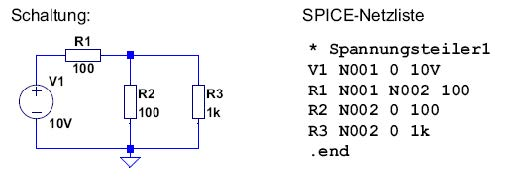
\includegraphics[scale=0.5]{pictures/page1.jpg}
  \end{center}

  Eine Netzliste repräsentiert eine Schaltung entsprechend Knoten- und Maschenregel. \newline Viele moderne SPICE Simulationsprogramme
  bieten dem Nutzer jedoch eine grafische Bedienoberfläche.
  So auch das in diesem Labor verwendete Programm, \textbf{LTspice XVII}.


\end{frame}

\begin{frame}[fragile]{Was ist LTspice - Installation \& Features}
  Die folgenden Punkte sind eingebettete Hyperlinks:
  \begin{enumerate}
    \item \href{https://www.analog.com/en/design-center/design-tools-and-calculators/ltspice-simulator.html}{Hier findet Ihr alle Infos vom Hersteller, \textbf{analog devices}}
    \item \href{http://ltspice.analog.com/software/LTspice.dmg}{Installer fuer MacOs http://ltspice.analog.com/software/LTspice.dmg}
    \item \href{http://ltspice.analog.com/software/LTspiceXVII.exe}{Installer fuer Windows http://ltspice.analog.com/software/LTspiceXVII.exe}
  \end{enumerate}

  \begin{center}

    \includemedia[
      width=0.6\linewidth,height=0.45\linewidth,
      addresource=pictures/LTspiceOverview.mp4, %two video files
      transparent, %transparent player background
      passcontext, %show VPlayer's right-click menu
      flashvars={
          source=pictures/LTspiceOverview.mp4
        }
    ]{}{VPlayer.swf}

  \end{center}
\end{frame}

\begin{frame}[fragile]{Ziel dieser Laborübung}

  \begin{enumerate}
    \item Erarbeiten der Grundlagen zur Simulation mit LTspice XVII
    \item Eigenständige Simulation von Schaltungen für Studien-/Abschlussarbeiten
    \item Verständnis theoretischer Inhalte mit empirischen Simulationen ergänzen
  \end{enumerate}

  \textbf{nächste Schritte}

  \begin{itemize}
    \item Übungen zum Einstieg in die Simulationswelt
    \item Schrittweise Erarbeitung eines Kleinprojektes \newline \textbf{Simulation einer Temperaturmessbrücke}
  \end{itemize}

\end{frame}

\begin{frame}[fragile]{LTspice XVII - Bitte öffnet alle das Programm}

  Die Benutzeroberfläche von LTspice XVII besteht aus den folgenden Elementen
  \begin{spacing}{0.6} \begin{tiny} \textbf{Hinweis:} Die Benutzeroberfläche von LTspice auf MacOS und Windows unterscheided sich leicht.
      Die Hautpmenuleiste ist für MacO nicht sichtbar.
    \end{tiny} \end{spacing}

  \begin{figure}
    \centering
    \subfloat[Hautpmenuleiste]{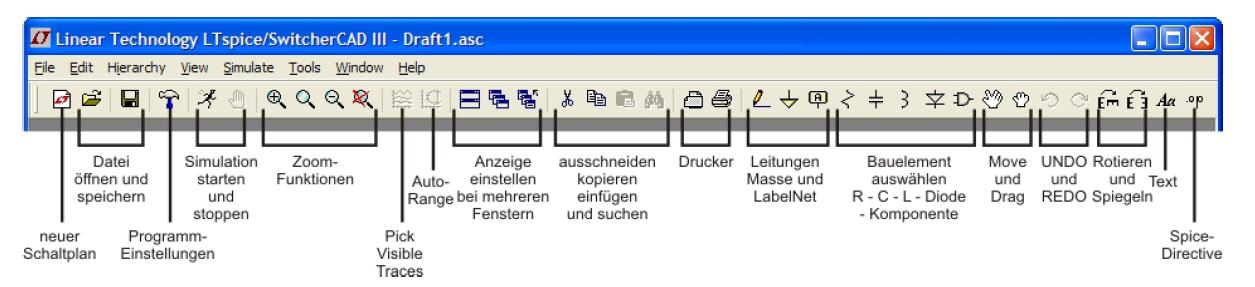
\includegraphics[scale=0.6]{pictures/mainmenu.jpg}}\\
    \subfloat[schematic]{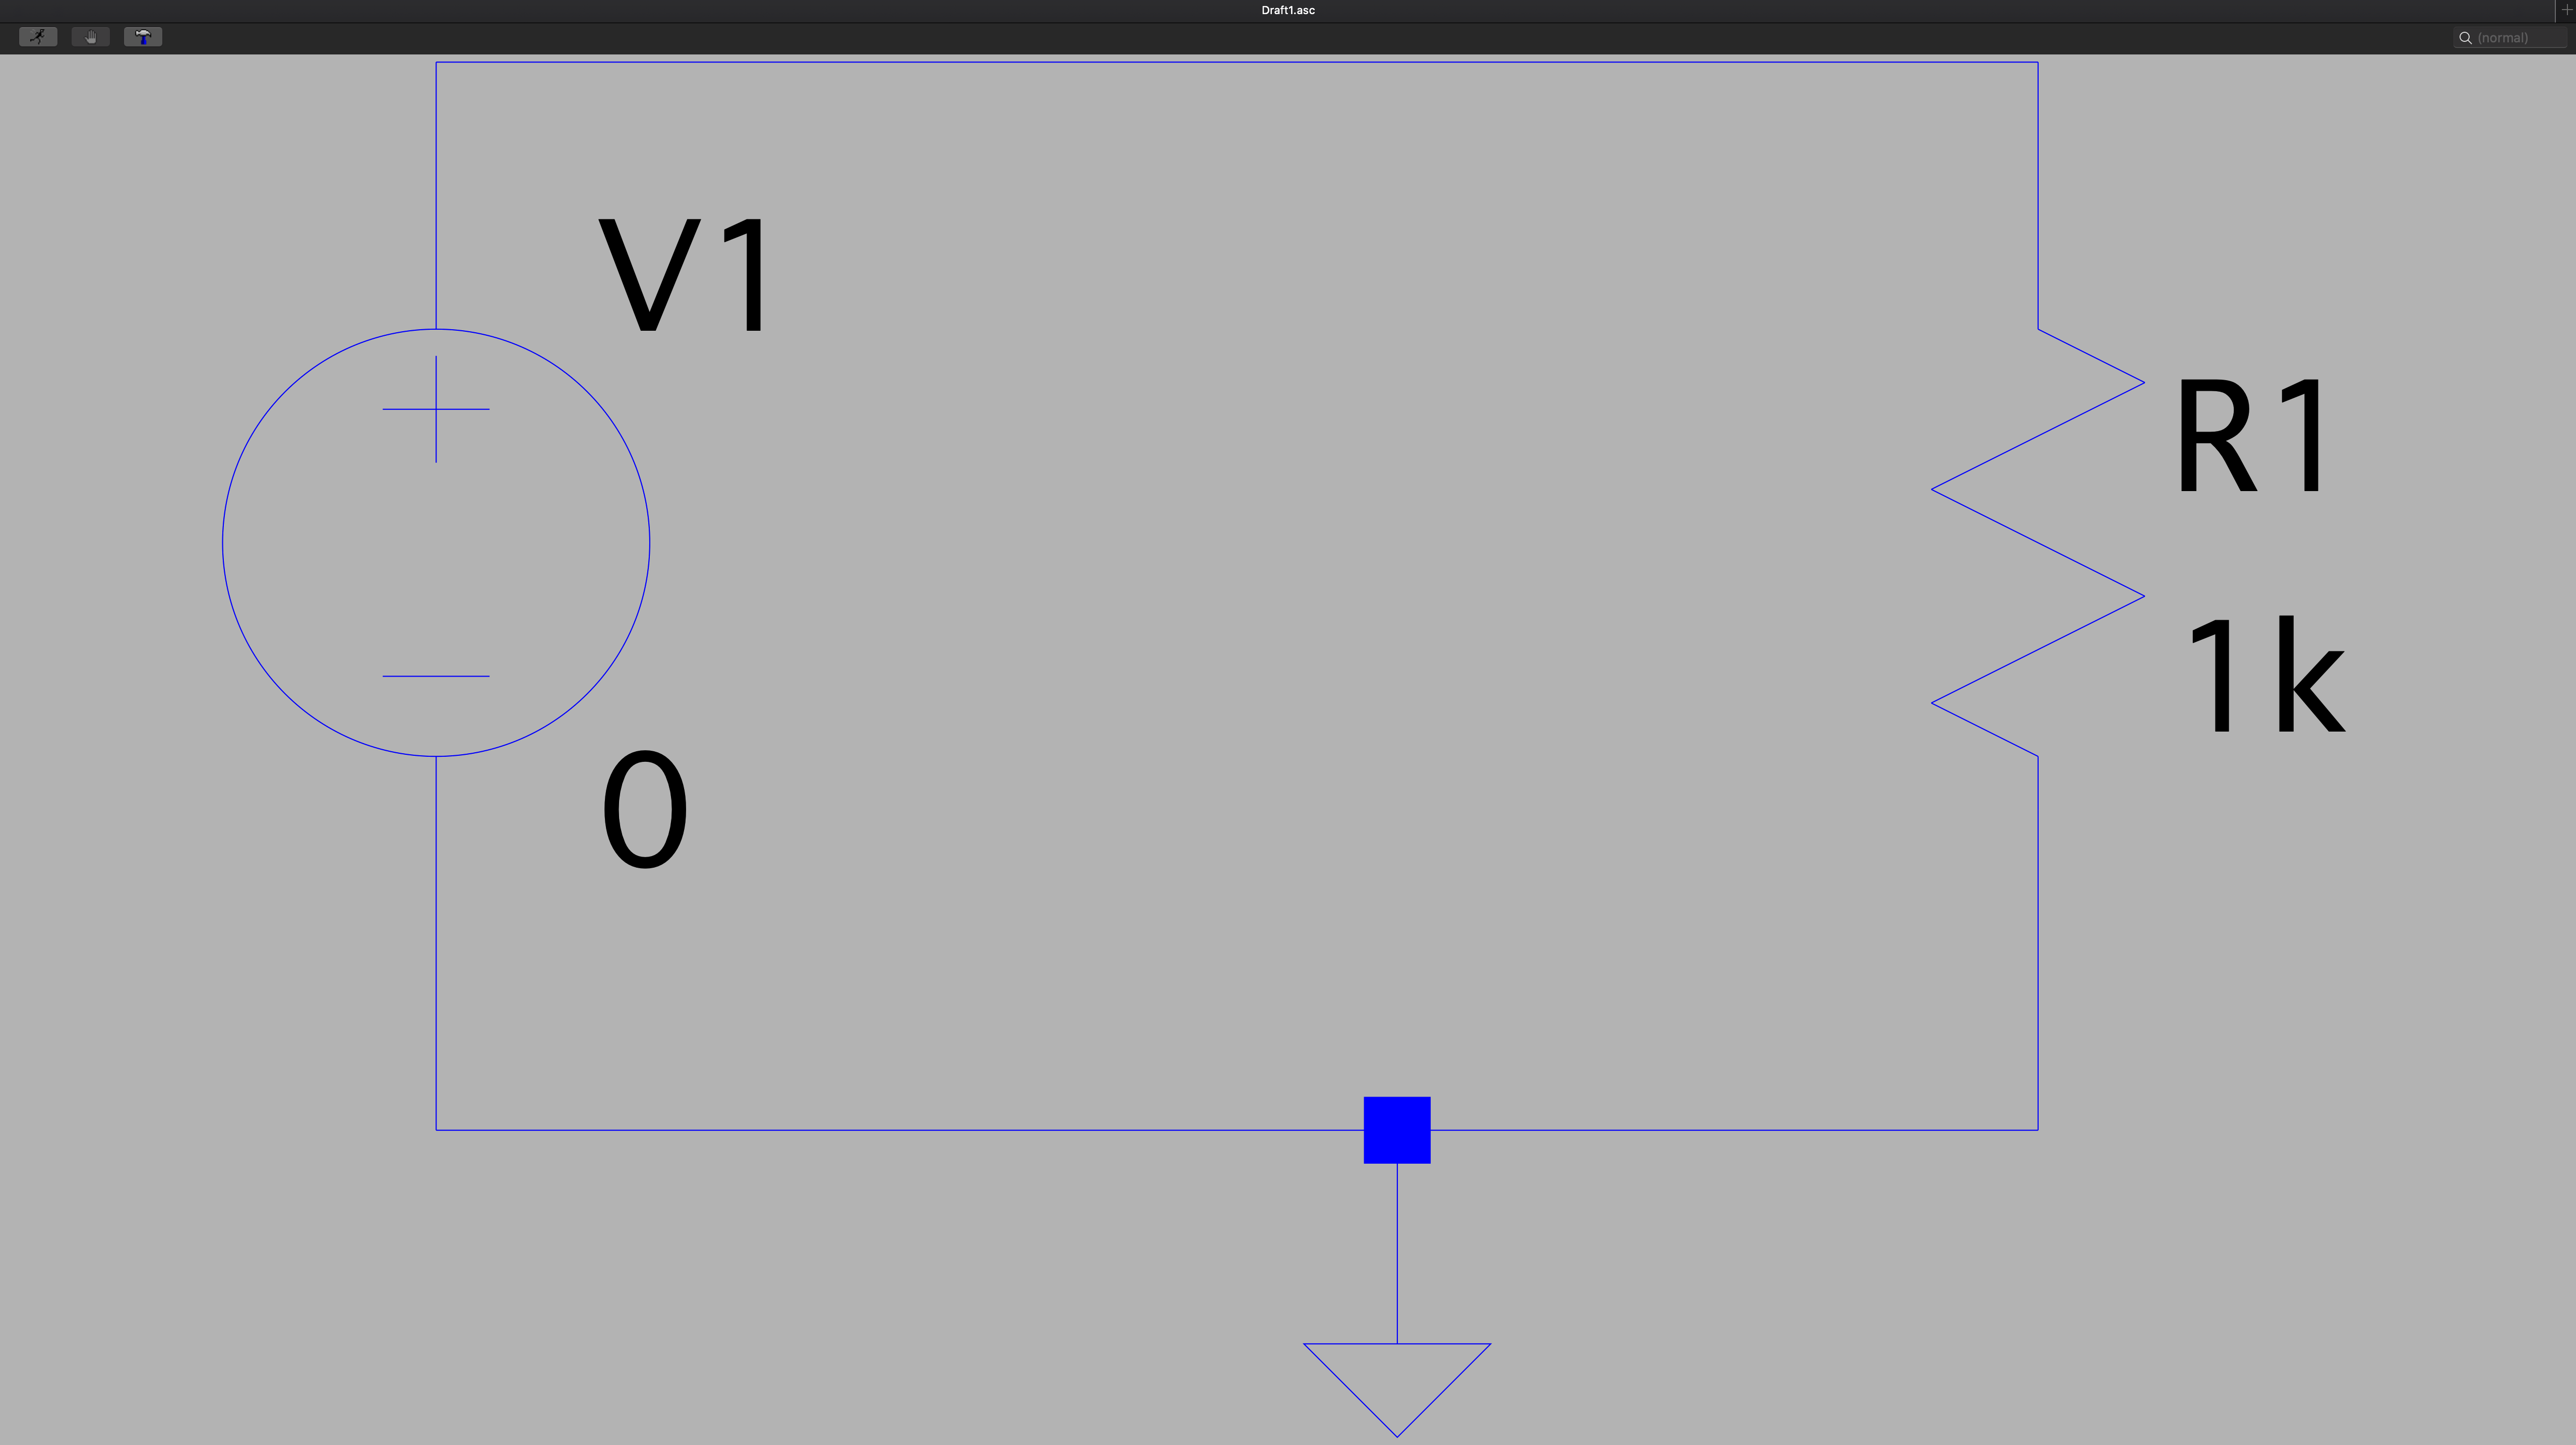
\includegraphics[width=4cm]{pictures/schematic.png}}\qquad
    \subfloat[waveform]{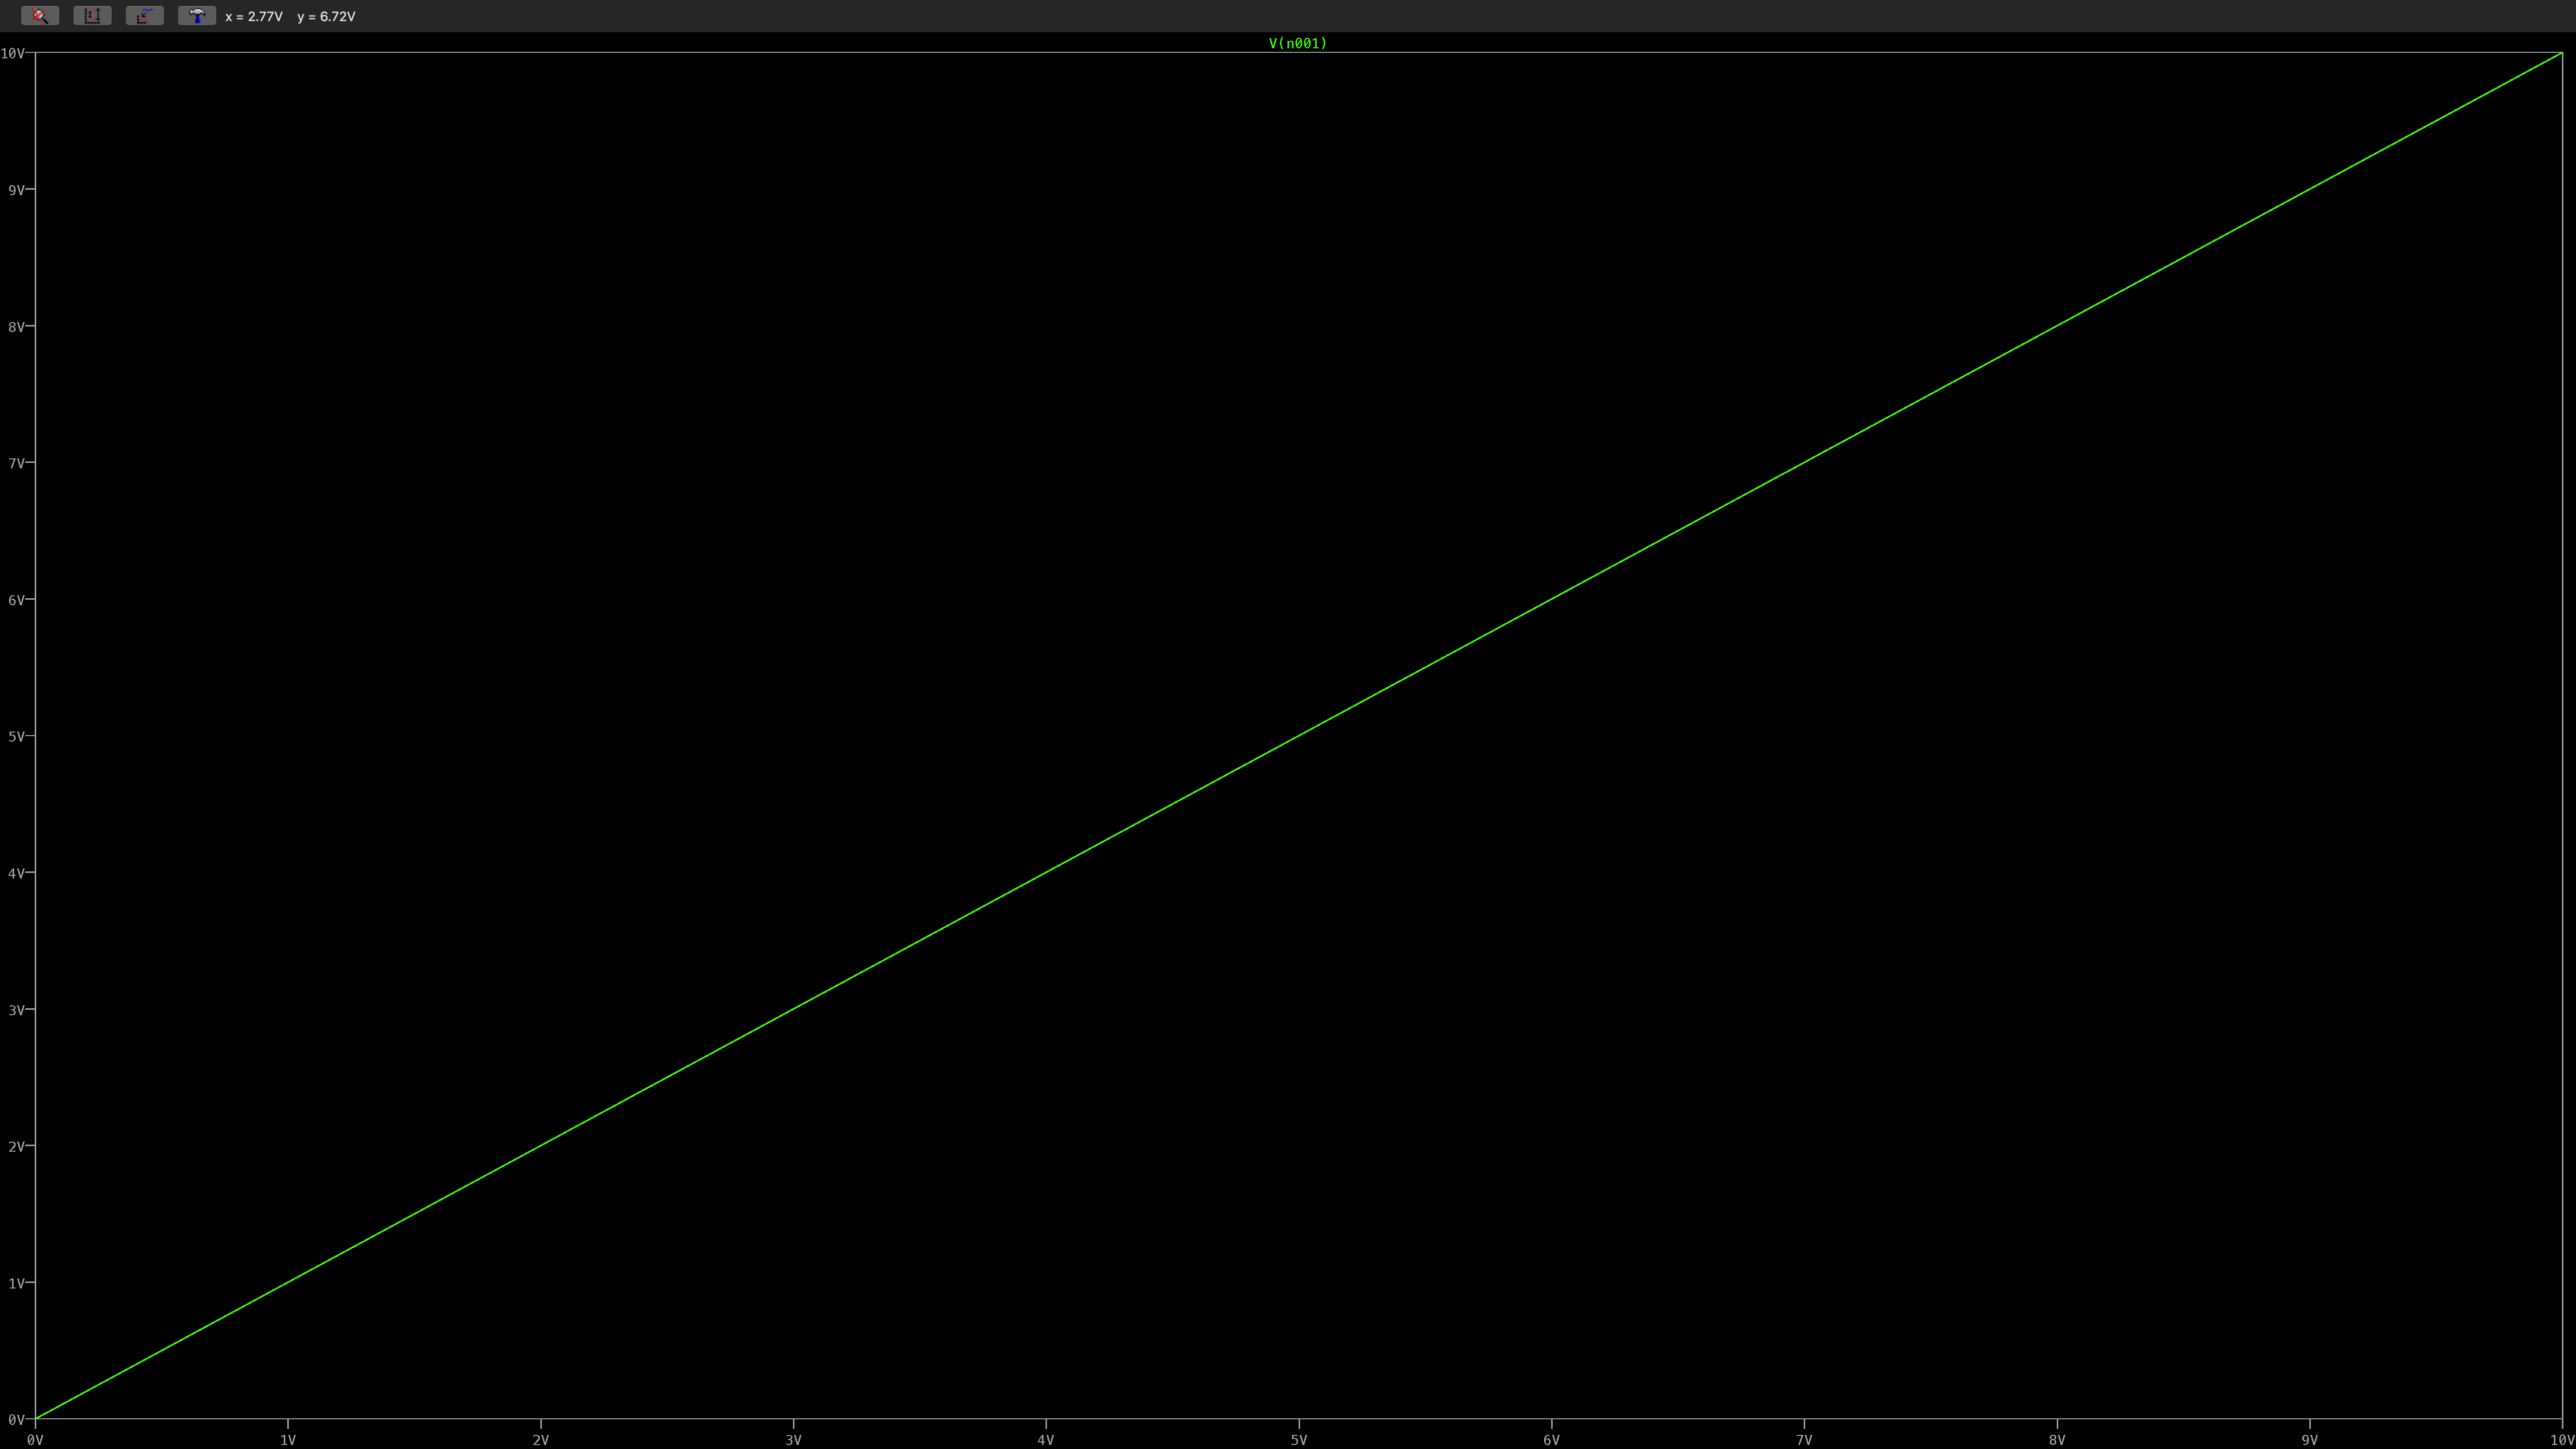
\includegraphics[width=4cm]{pictures/waveform.png}}
  \end{figure}

\end{frame}

\begin{frame}{LTspice XVII - Überblick Simulationsarten}

  Die Simulationsart kann im Menu \textbf{Simulation Command} konfiguriert werden.

  \begin{figure}
    \centering
    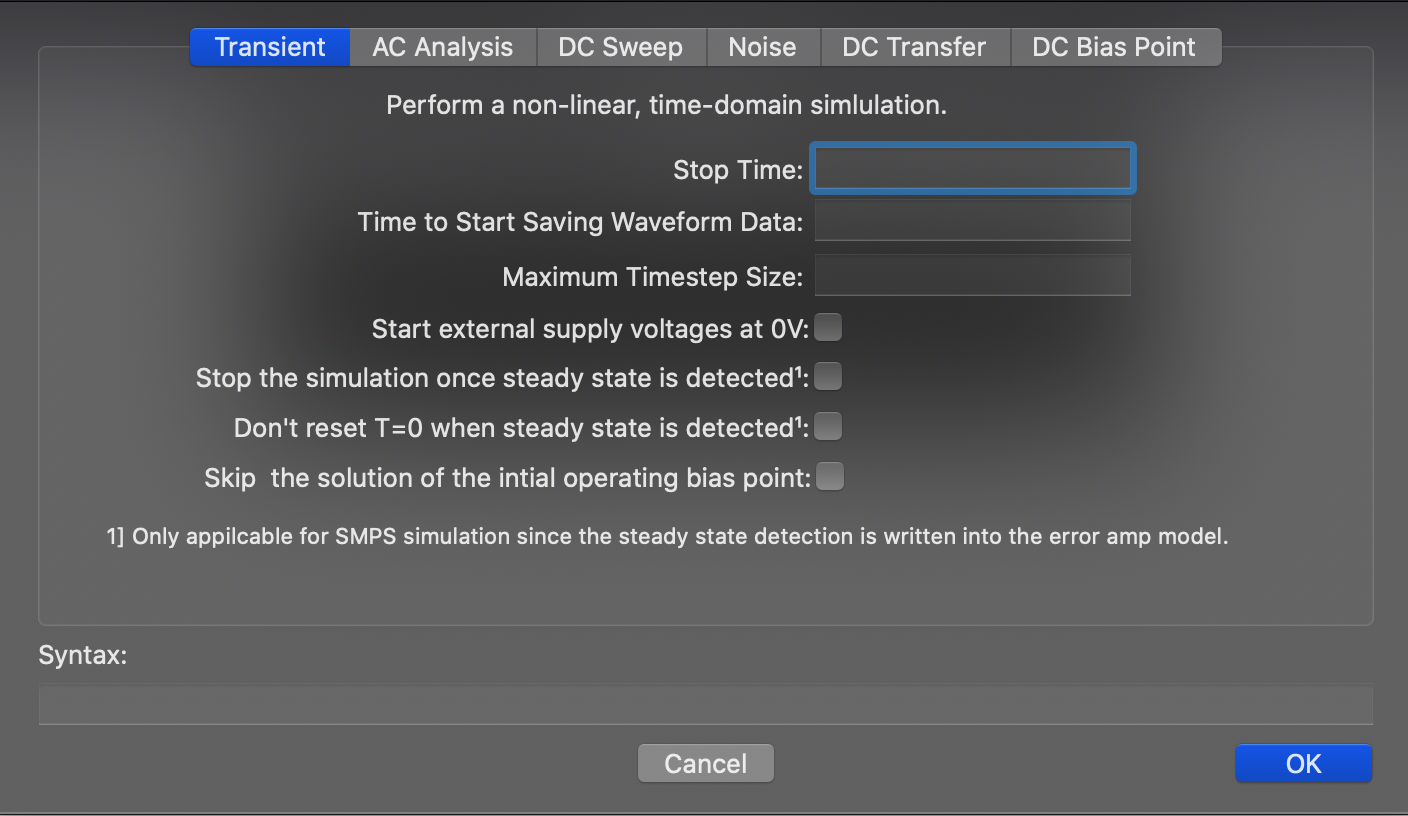
\includegraphics[width=10cm]{pictures/simulationcmd.png}
  \end{figure}

\end{frame}

\begin{frame}{LTspice XVII - Überblick Simulationsarten}

  \begin{scriptsize}
    \begin{tabular}{ l }
      \hline
      \textbf{Transient}                                                                       \\
      Analyse einer Schaltung \textbf{über die Zeit}, z.B. zur Analyse von Einschwingvorgängen \\
      \hline
      \textbf{AC Analysis}                                                                     \\
      Analyse einer Schaltung \textbf{unter Variation der Frequenz},                           \\ z.B. zur Analyse von Grenzfrequenzen\\
      \hline
      \textbf{DC Sweep}                                                                        \\
      Analyse einer Schaltung \textbf{unter Variation der Spannung},                           \\ z.B. zur Analyse von Bauteilkennlinien\\
      \hline
      \textbf{Operation Point}                                                                 \\
      Analyse des \textbf{Arbeitspunktes} einer Schaltung \textbf{ohne Variation}              \\
      \hline
      \textbf{Noise}                                                                           \\
      Analyse von Rauschverhalten, Bauteilfehlern oder z.B. EMV Einflüssen                     \\
      \hline
      \textbf{DC Transfer}                                                                     \\
      Analyse der DC-Übertragungsfunktion einer Schaltung                                      \\
      \hline
      \textbf{DC Bias Point}                                                                   \\
      Analyse des Arbeitspunktes einer Schaltung ohne dynamisches Verhalten                    \\
      \hline
    \end{tabular}
  \end{scriptsize}

\end{frame}

\begin{frame}[fragile]{Nützliche Voreinstellungen}

  Die Farbdarstellung von LTspice kann jederzeit konfiguriert werden. Geht dazu über das
  \textbf{control panel} Feld, 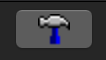
\includegraphics[scale=0.5]{pictures/controlpanel.png} in die Farbeinstellungen
  (\textbf{configure colors}). Hier könnt ihr flexibel die Farbdarstellung konfigurieren.

  \begin{figure}
    \centering
    \subfloat{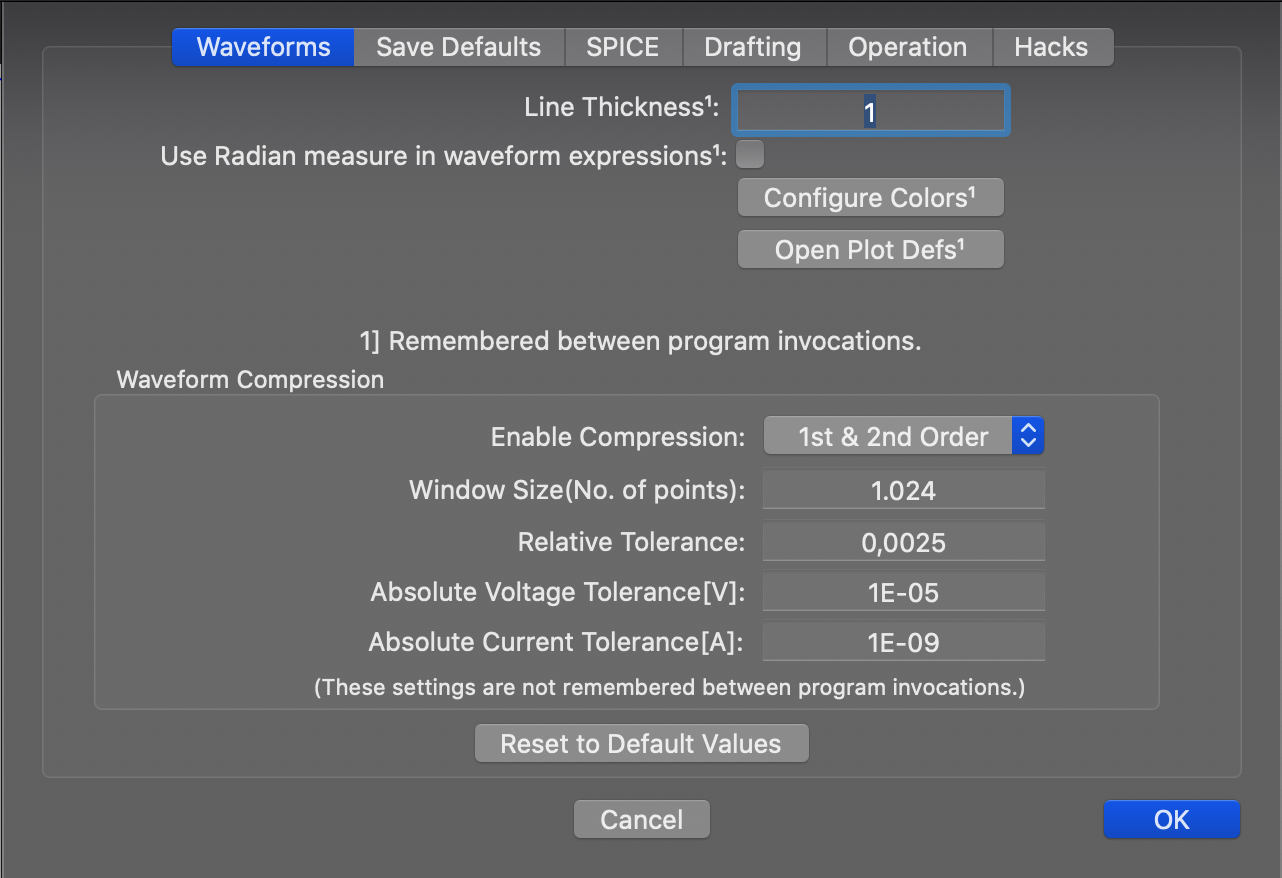
\includegraphics[width=5.5cm]{pictures/controlpanel_2.png}}\qquad
    \subfloat{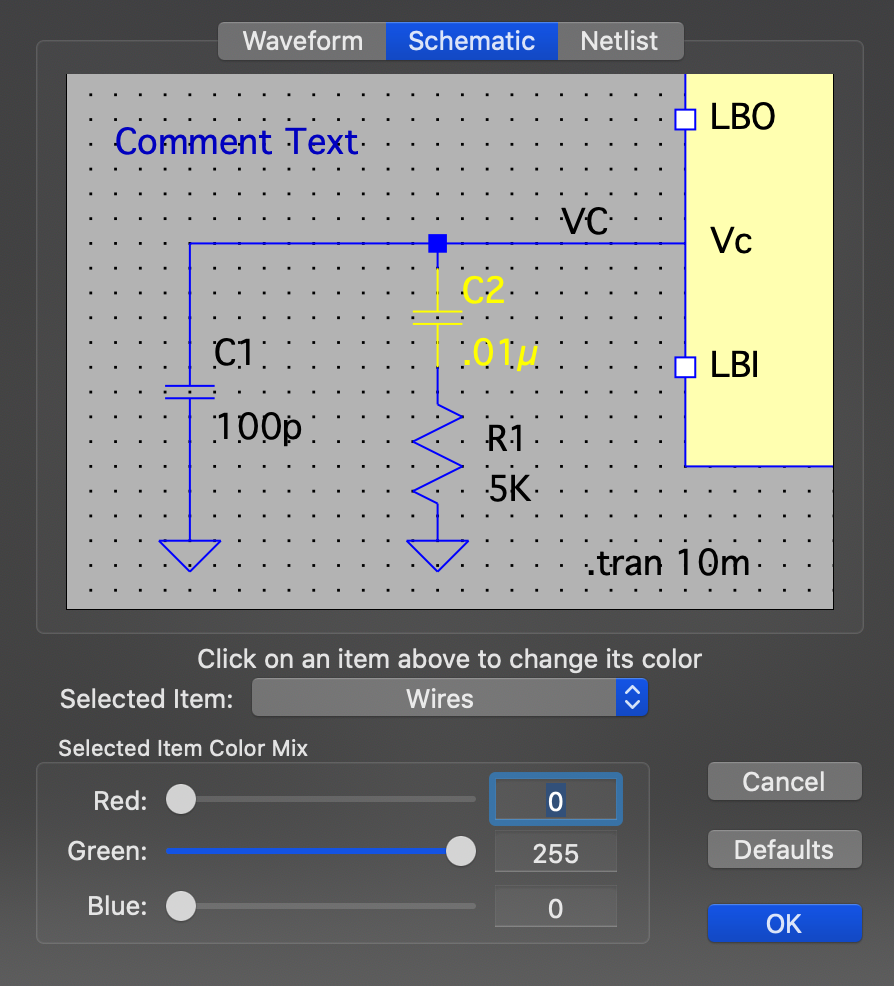
\includegraphics[width=3.5cm]{pictures/colorcfg.png}}
  \end{figure}

\end{frame}

\begin{frame}[t]{Shortkeys}

  Es gibt eine gute Übersicht von HotKeys die die Arbeit mit LTspice deutlich effektiver macht (nachfolgend sind Hyperlinks embedded).

  \begin{itemize}
    \item \href{https://www.analog.com/media/en/simulation-models/spice-models/LTspice_ShortcutFlyer.pdf?modelType=spice-models}{Windows ShortKeys}.
    \item \href{https://www.analog.com/media/en/simulation-models/spice-models/LTspiceShortcutsForMacOSX.pdf?modelType=spice-models}{MacOS ShortKeys}.
    \item \href{https://www.analog.com/media/en/simulation-models/spice-models/LTspiceGettingStartedGuide.pdf?modelType=spice-models}{LTspice getting started guide}.
  \end{itemize}

  \begin{figure}
    \centering
    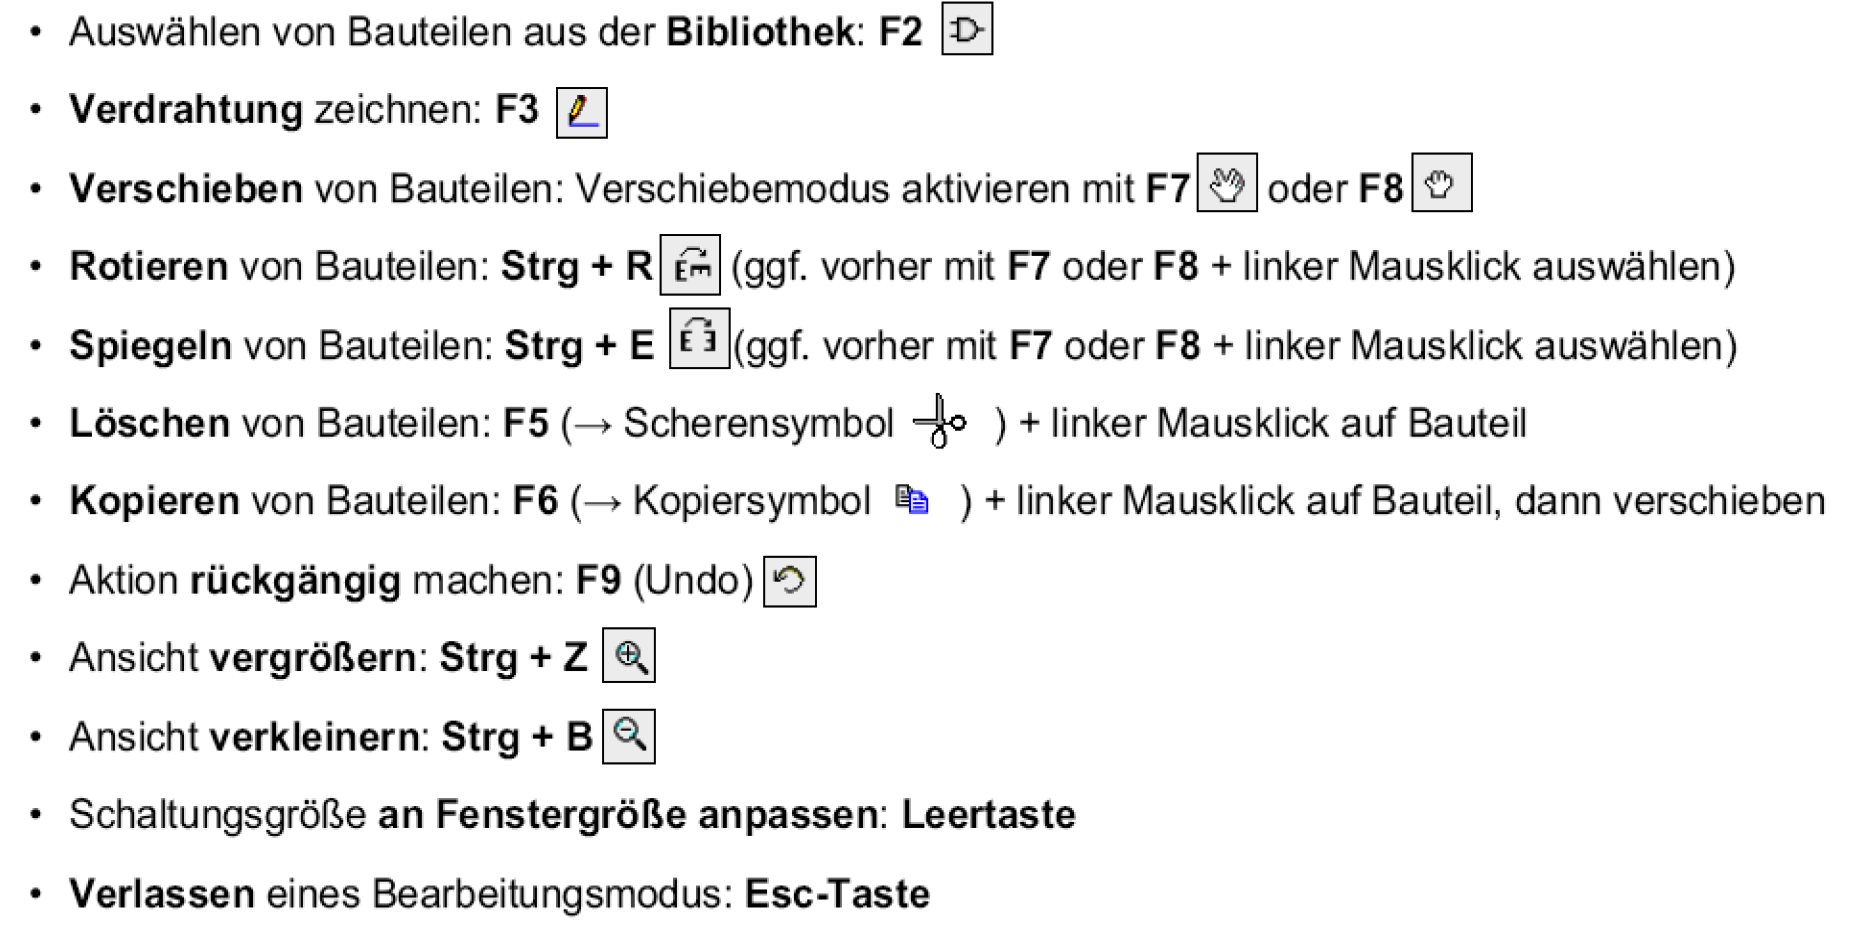
\includegraphics[scale=0.25]{pictures/shortkeys.png}
  \end{figure}

\end{frame}

\begin{frame}[t]{Nützliche Hinweise}

  \begin{itemize}
    \item Zahlenwerte immer mit \textbf{Dezimalpunkt statt Komma eingeben! 3.5 anstatt 3,5!}
    \item SPICE arbeitet nach dem Knotenpotenzialverfahren - \textbf{Es muss immer ein Bezugsknoten
            (Masse, Ground) angegeben werden,} sonst treten Simulationsfehler auf (Achtung: Es erfolgt
          keine Fehlermeldung!).
  \end{itemize}
  Achtet darauf die korrekten Suffixe für Einheiten zu verwenden.

  \begin{tabular}{| c | c | c | c | c | c | c | c | c | c |}
    \hline
    Terra    & Giga    & Mega    & Kilo    & milli    & micro    & nano     & pico      & femto     \\
    \hline
    T        & G       & Meg     & K       & m        & u        & n        & p         & f         \\
    \hline
    $e^{12}$ & $e^{9}$ & $e^{6}$ & $e^{3}$ & $e^{-3}$ & $e^{-6}$ & $e^{-9}$ & $e^{-12}$ & $e^{-15}$ \\
    \hline
  \end{tabular}
\end{frame}

\section{Hands-on LTspice - Das Labor beginnt}


\begin{frame}[fragile]{Vorgehensweise}

  Diese Übungen sind zur interaktiven Arbeit mit LTspice gedacht.
  Sie führen von der Aufgabe über den Lösungsansatz bis hin zur fertigen Analyse.

  Bitte geht nach den folgenden Schritten vor, um die Übungen strukturiert zu bearbeiten.

  \begin{enumerate}
    \item \textbf{Schematic modellieren}
    \item \textbf{Simulationsart analysieren}
    \item \textbf{Simulationsart konfigurieren}
    \item \textbf{Ergebnis mit der Vorgabe abgleichen}
  \end{enumerate}

  Sollte es zu Problemen kommen, bitten wir euch uns direkt einen Hinweis zu geben!

\end{frame}

\section{Übungen}

\begin{frame}[t]{ohmscher Widerstand}

    \textbf{Ziel - Darstellung von Bauteilkennlinie}
    
    \begin{spacing}{0.6} \begin{tiny}
    
    Das ohmsche Gesetz $U=R I$ lässt sich mit Hilfe eines kleinen Schaltungsexperimentes gut visualisieren und nachvollziehen. 
    Hierzu werden wir die folgende Schaltung aufbauen und den Stromverlauf über dem Widerstand darstellen. 
    \end{tiny} \end{spacing}
    \begin{spacing}{0.9} \begin{tiny}
    \begin{table}[h!]
      \begin{tabular}{p{3cm} p{7cm}}
        \hline
        \textbf{Erstellung des Schaltplans} & \\
        \hline \\
        \begin{minipage}{.3\textwidth}
          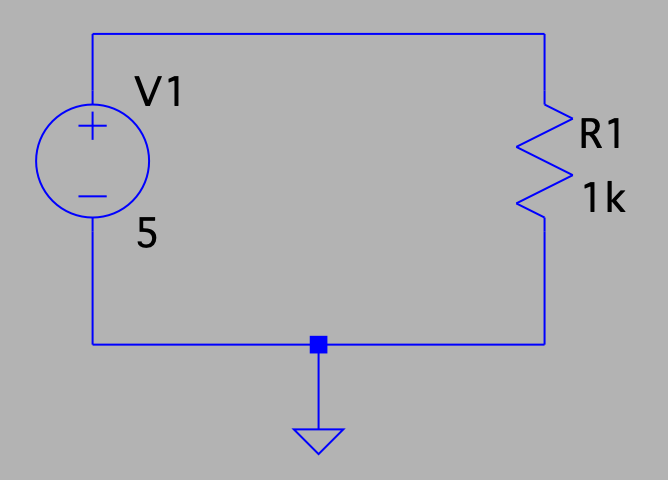
\includegraphics[width=\linewidth]{pictures/res.png}
        \end{minipage} 
        & 
        \begin{minipage}{.7\textwidth}
        \begin{itemize}
          \item Erstellt ein neues schematic (File $->$ new schematic)
          \item Speichert es direkt als neue Dateil ab (File $->$ save as)
          \item Öffnet den Bauteileditor (\textbf{F2}) und für eine Spannungsquelle hinzu (voltage)
          \item Öffnet erneut den Bauteileditor und für einen Widerstand hinzu (resistor bzw. EuropeanResistor fuer die bekannte Box-Darstellung)
          \item Fügt einen Masseknoten als Bezugsknoten hinzu (\textbf{F4}).
          \item Verdrahtet die Schaltung (\textbf{F3})
        \end{itemize}
        \end{minipage} 
        \\
         & \\
         \hline
         \textbf{Konfiguration der Simulation} & \\
         \hline \\
         \begin{minipage}{.3\textwidth}
          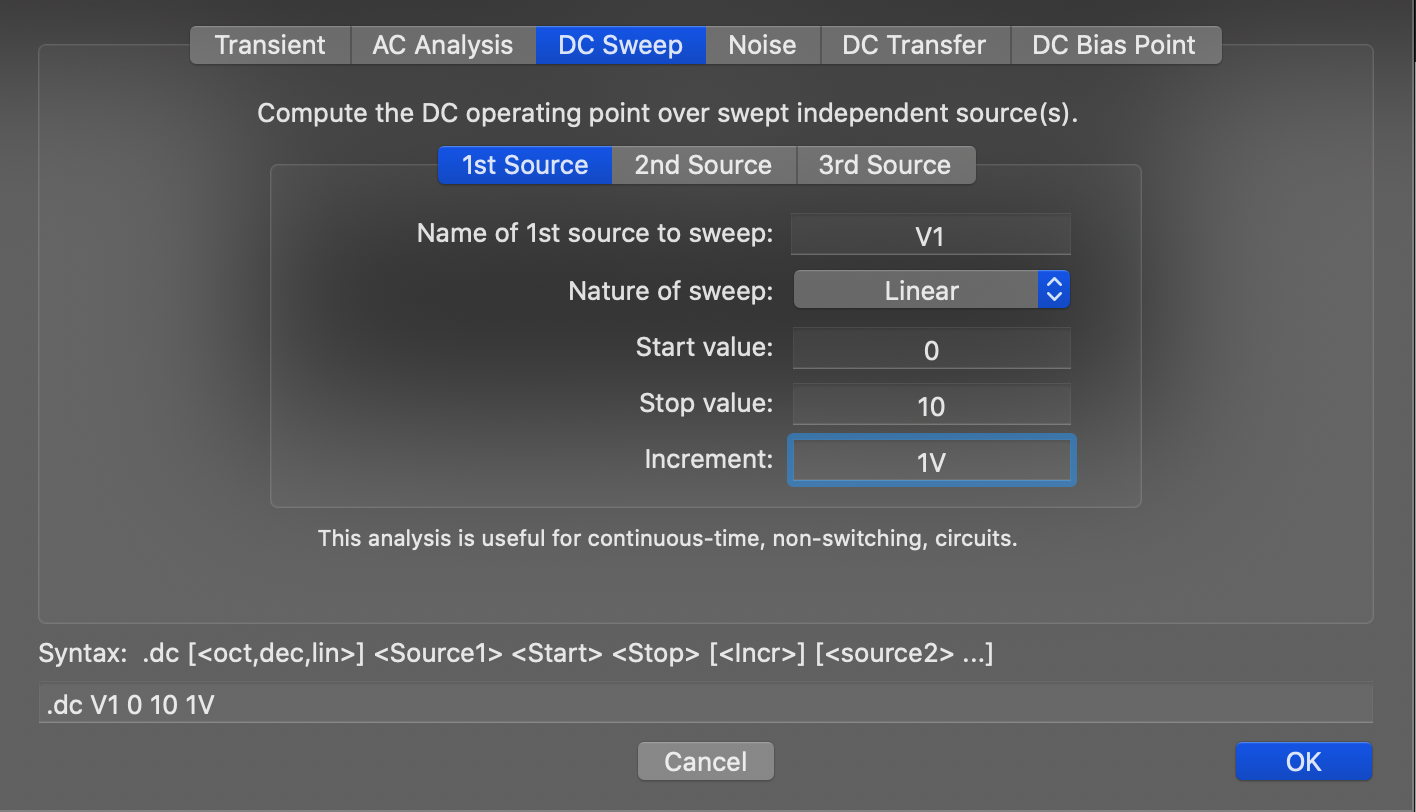
\includegraphics[width=\linewidth]{pictures/simulationcmd_1.png}
        \end{minipage} 
        & 
        \begin{minipage}{.7\textwidth}
        \begin{itemize}
          \item Im Menu Simulation, wählt \textbf{Edit simulation command} und wählt den DC Sweep. 
          \item Unser Ziel ist es den Stromverlauf über dem Widerstand zu simulieren
          \item Daher konfigurieren wir die Spannungsquelle \textbf{V1} mit einem \textbf{linearen} Sweep von 0 bis 10 V mit einer \textbf{Schrittweite} von 1V.
          \item Bestätigt mit \textit{OK} und fügt die Sumlationsansweisung dem schematic hinzu
        \end{itemize}
        \end{minipage} 
        \\
         & \\
         \hline
      \end{tabular}
    
    \end{table}
    
    \end{tiny} \end{spacing}
    
     \end{frame}
    
     \begin{frame}[t]{ohmscher Widerstand}
    
      \begin{spacing}{0.9} \begin{tiny}
      \begin{table}[h!]
        \begin{tabular}{p{5cm} p{5cm}}
          \hline
          \textbf{Simulation und Analyse} & \\
          \hline \\
          \begin{minipage}{.5\textwidth}
            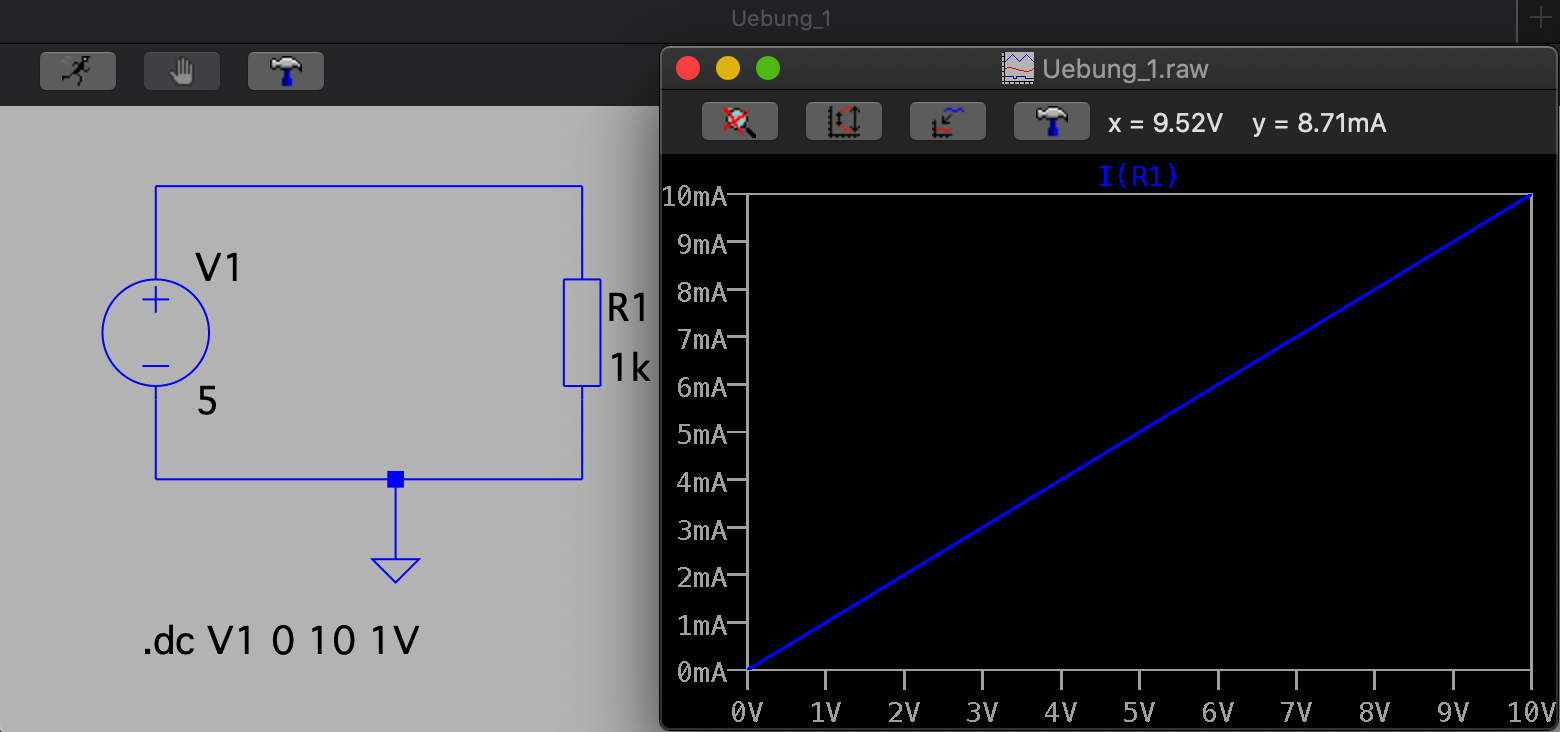
\includegraphics[width=\linewidth]{pictures/analysis.png}
          \end{minipage} 
          & 
          \begin{minipage}{.5\textwidth}
          \begin{itemize}
            \item Klickt auf 
\includegraphics[scale=0.3]{pictures/run.png} (run) und LTspice startet die Simulation
            \item Der waveform viewer öffnet sich - ihr könnt auf zwei Arten Strom, Spannung und Leistungen aus eurer Schaltung anzeigen lassen. \newline\newline
            \textbf{Im schematic} könnt ihr über ein Bauteil mit der Maus fahren und es erscheint eine Stromzange\newline\newline
            \textbf{Im schematic} könnt ihr über ein Bauteil mit der Maus fahren, Shift gedrückt halten und es erscheint eine Leistungsmessanzeige\newline\newline
            \textbf{Im schematic} könnt ihr über eine Knoten mit der Maus fahren und es erscheint ein Spannungsmesser\newline\newline
            \textbf{Im waveform viewer} könnt ihr über rechten Mausklick $->$ add trace die verfügbaren Messtellen direkt auswählen
            \item Wir wählen \textbf{I(R1)}, den Strom durch unseren Widerstand R1. 
          \end{itemize}
          \end{minipage} 
          \\
        \end{tabular}
      \end{table}
    \end{tiny} \end{spacing}
    
      \begin{spacing}{0.9} \begin{tiny}
        \begin{table}[h!]
          \begin{tabular}{p{10cm} }
            \hline
            \textbf{Ergebnis und Auswertung} \\
            \hline \\    
            Wie zu erwarten liefert dieses einfache Beispiel den Zusammenhang zwischen Strom, Spannung und Widerstand. Probiert an dieser Stelle gerne die Spannung, Schrittweite
            zu variieren oder weitere Werte im waveform viewer anzueigen zu lassen.
          \end{tabular}
        \end{table}
      \end{tiny} \end{spacing}
      
       \end{frame}%resistor
\begin{frame}[t]{Diode}

    \textbf{Ziel - Darstellung von Bauteilkennlinie}
    
    \begin{spacing}{0.6} \begin{tiny}
    
    Eine Diode wird oft durch Ihre Durchlassspannung klassifiziert. Dies ist die Spannung ab der die Diode leitend wird. Leitend ist Sie, wenn ein Strom fließt. Dieses Verhalten möchten
    wir in einem kleinen simulativen Experiment herausarbeiten. 
    \end{tiny} \end{spacing}
    \begin{spacing}{0.9} \begin{tiny}
    \begin{table}[h!]
      \begin{tabular}{p{3cm} p{7cm}}
        \hline
        \textbf{Erstellung des Schaltplans} & \\
        \hline \\
        \begin{minipage}{.3\textwidth}
          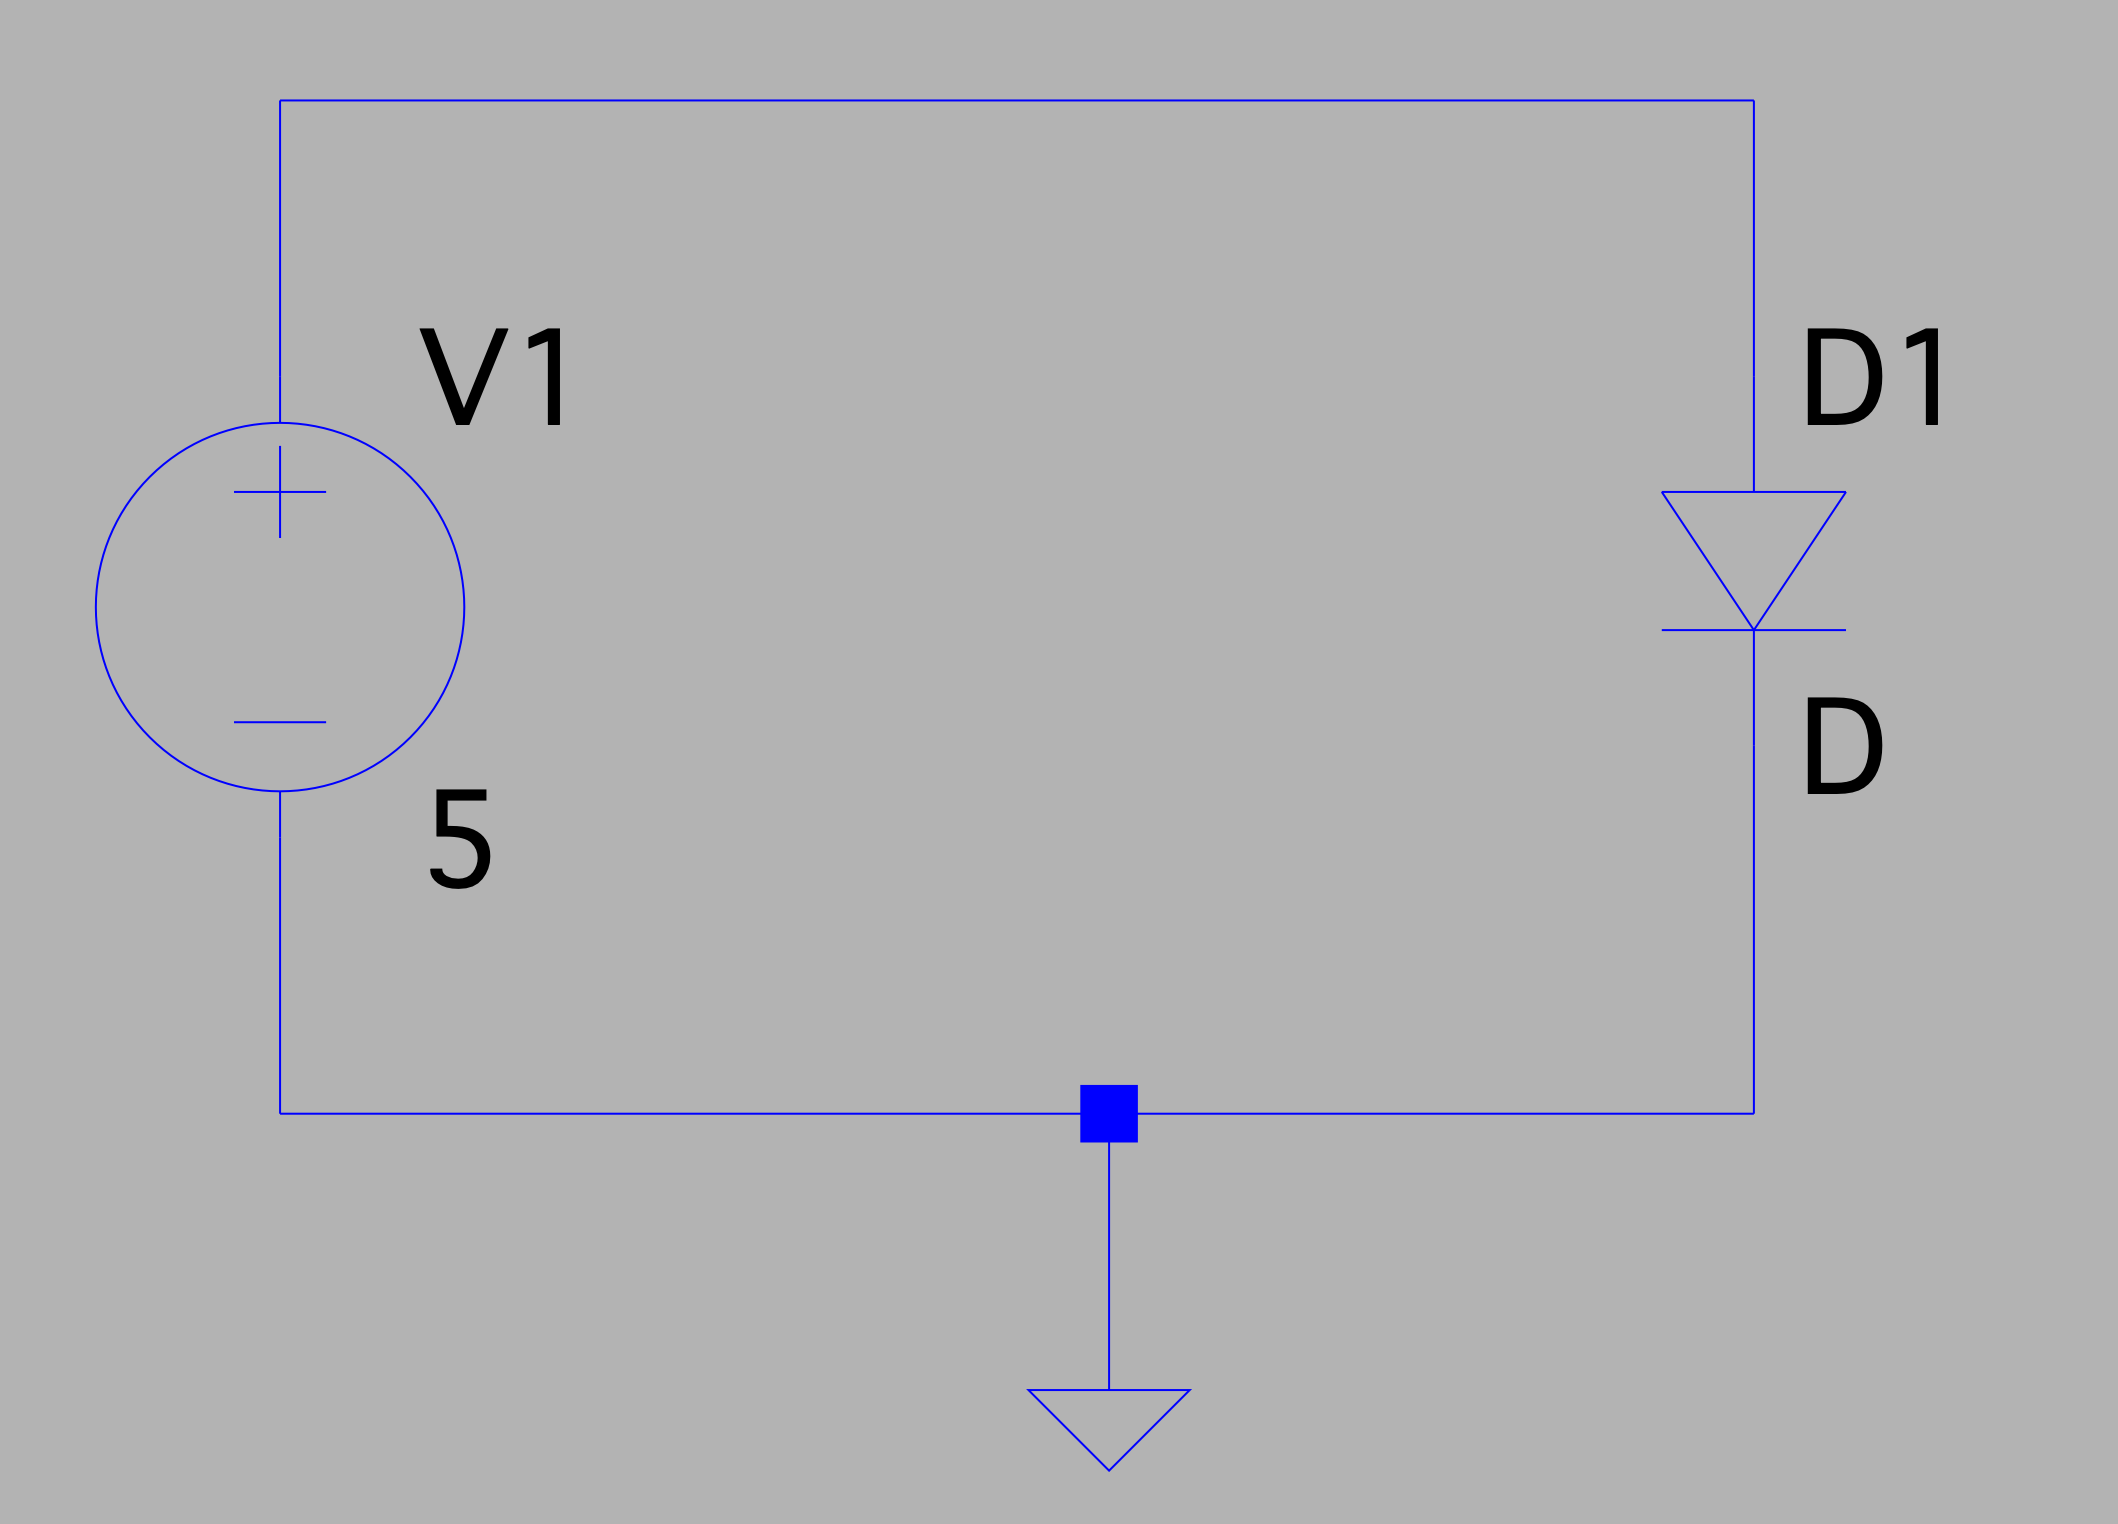
\includegraphics[width=\linewidth]{pictures/diode.png}
        \end{minipage} 
        & 
        \begin{minipage}{.7\textwidth}
        \begin{itemize}
          \item Speichert das Projekt direkt als neue Datei ab (File $->$ save as ) 
          \item Löscht den Wiederstand heraus (\textbf{F5}) 
          \item Öffnet erneut den Bauteileditor (\textbf{F2}) und für eine einfache Diode hinzu (sucht nach Diode \dots)
          \item Verdrahtet die Schaltung wieder vollstänndig (\textbf{F3})
        \end{itemize}
        \end{minipage} 
        \\
         & \\
         \hline
         \textbf{Konfiguration der Simulation} & \\
         \hline \\
         \begin{minipage}{.3\textwidth}
          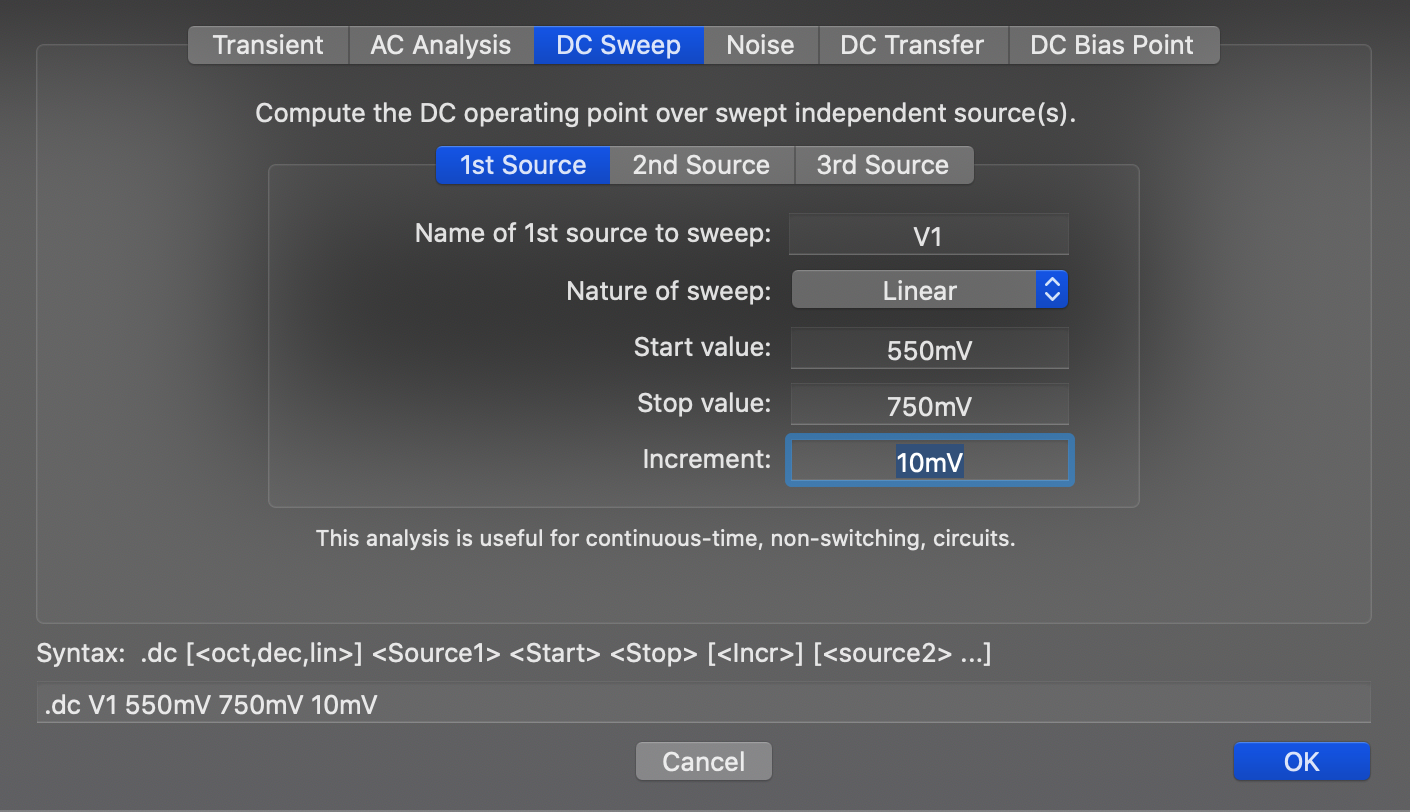
\includegraphics[width=\linewidth]{pictures/simulationcmd_2.png}
        \end{minipage} 
        & 
        \begin{minipage}{.7\textwidth}
        \begin{itemize}
          \item Im Menu Simulation, wählt \textbf{Edit simulation command} und bliebt beim DC Sweep. 
          \item Unser Ziel ist es den Stromverlauf durch die Diode zu messen. Dafür müssen wir die Spannung erhöhen. 
          Wir wissen, dass die notwendige Spannung im Bereich 600 - 700 mV liegen muss. 
          \item Daher konfigurieren wir die Spannungsquelle \textbf{V1} mit einem \textbf{linearen} Sweep von 550 bis 750 mV mit einer \textbf{Schrittweite} von 10 mV.
          \item Bestätigt mit \textit{OK} und fügt die Sumlationsansweisung dem schematic hinzu
        \end{itemize}
        \end{minipage} 
        \\
         & \\
         \hline
      \end{tabular}
    
    \end{table}
    
    \end{tiny} \end{spacing}
    
     \end{frame}
    
     \begin{frame}[t]{Diode}
    
      \begin{spacing}{0.9} \begin{tiny}
      \begin{table}[h!]
        \begin{tabular}{p{5cm} p{5cm}}
          \hline
          \textbf{Simulation und Analyse} & \\
          \hline \\
          \begin{minipage}{.5\textwidth}
            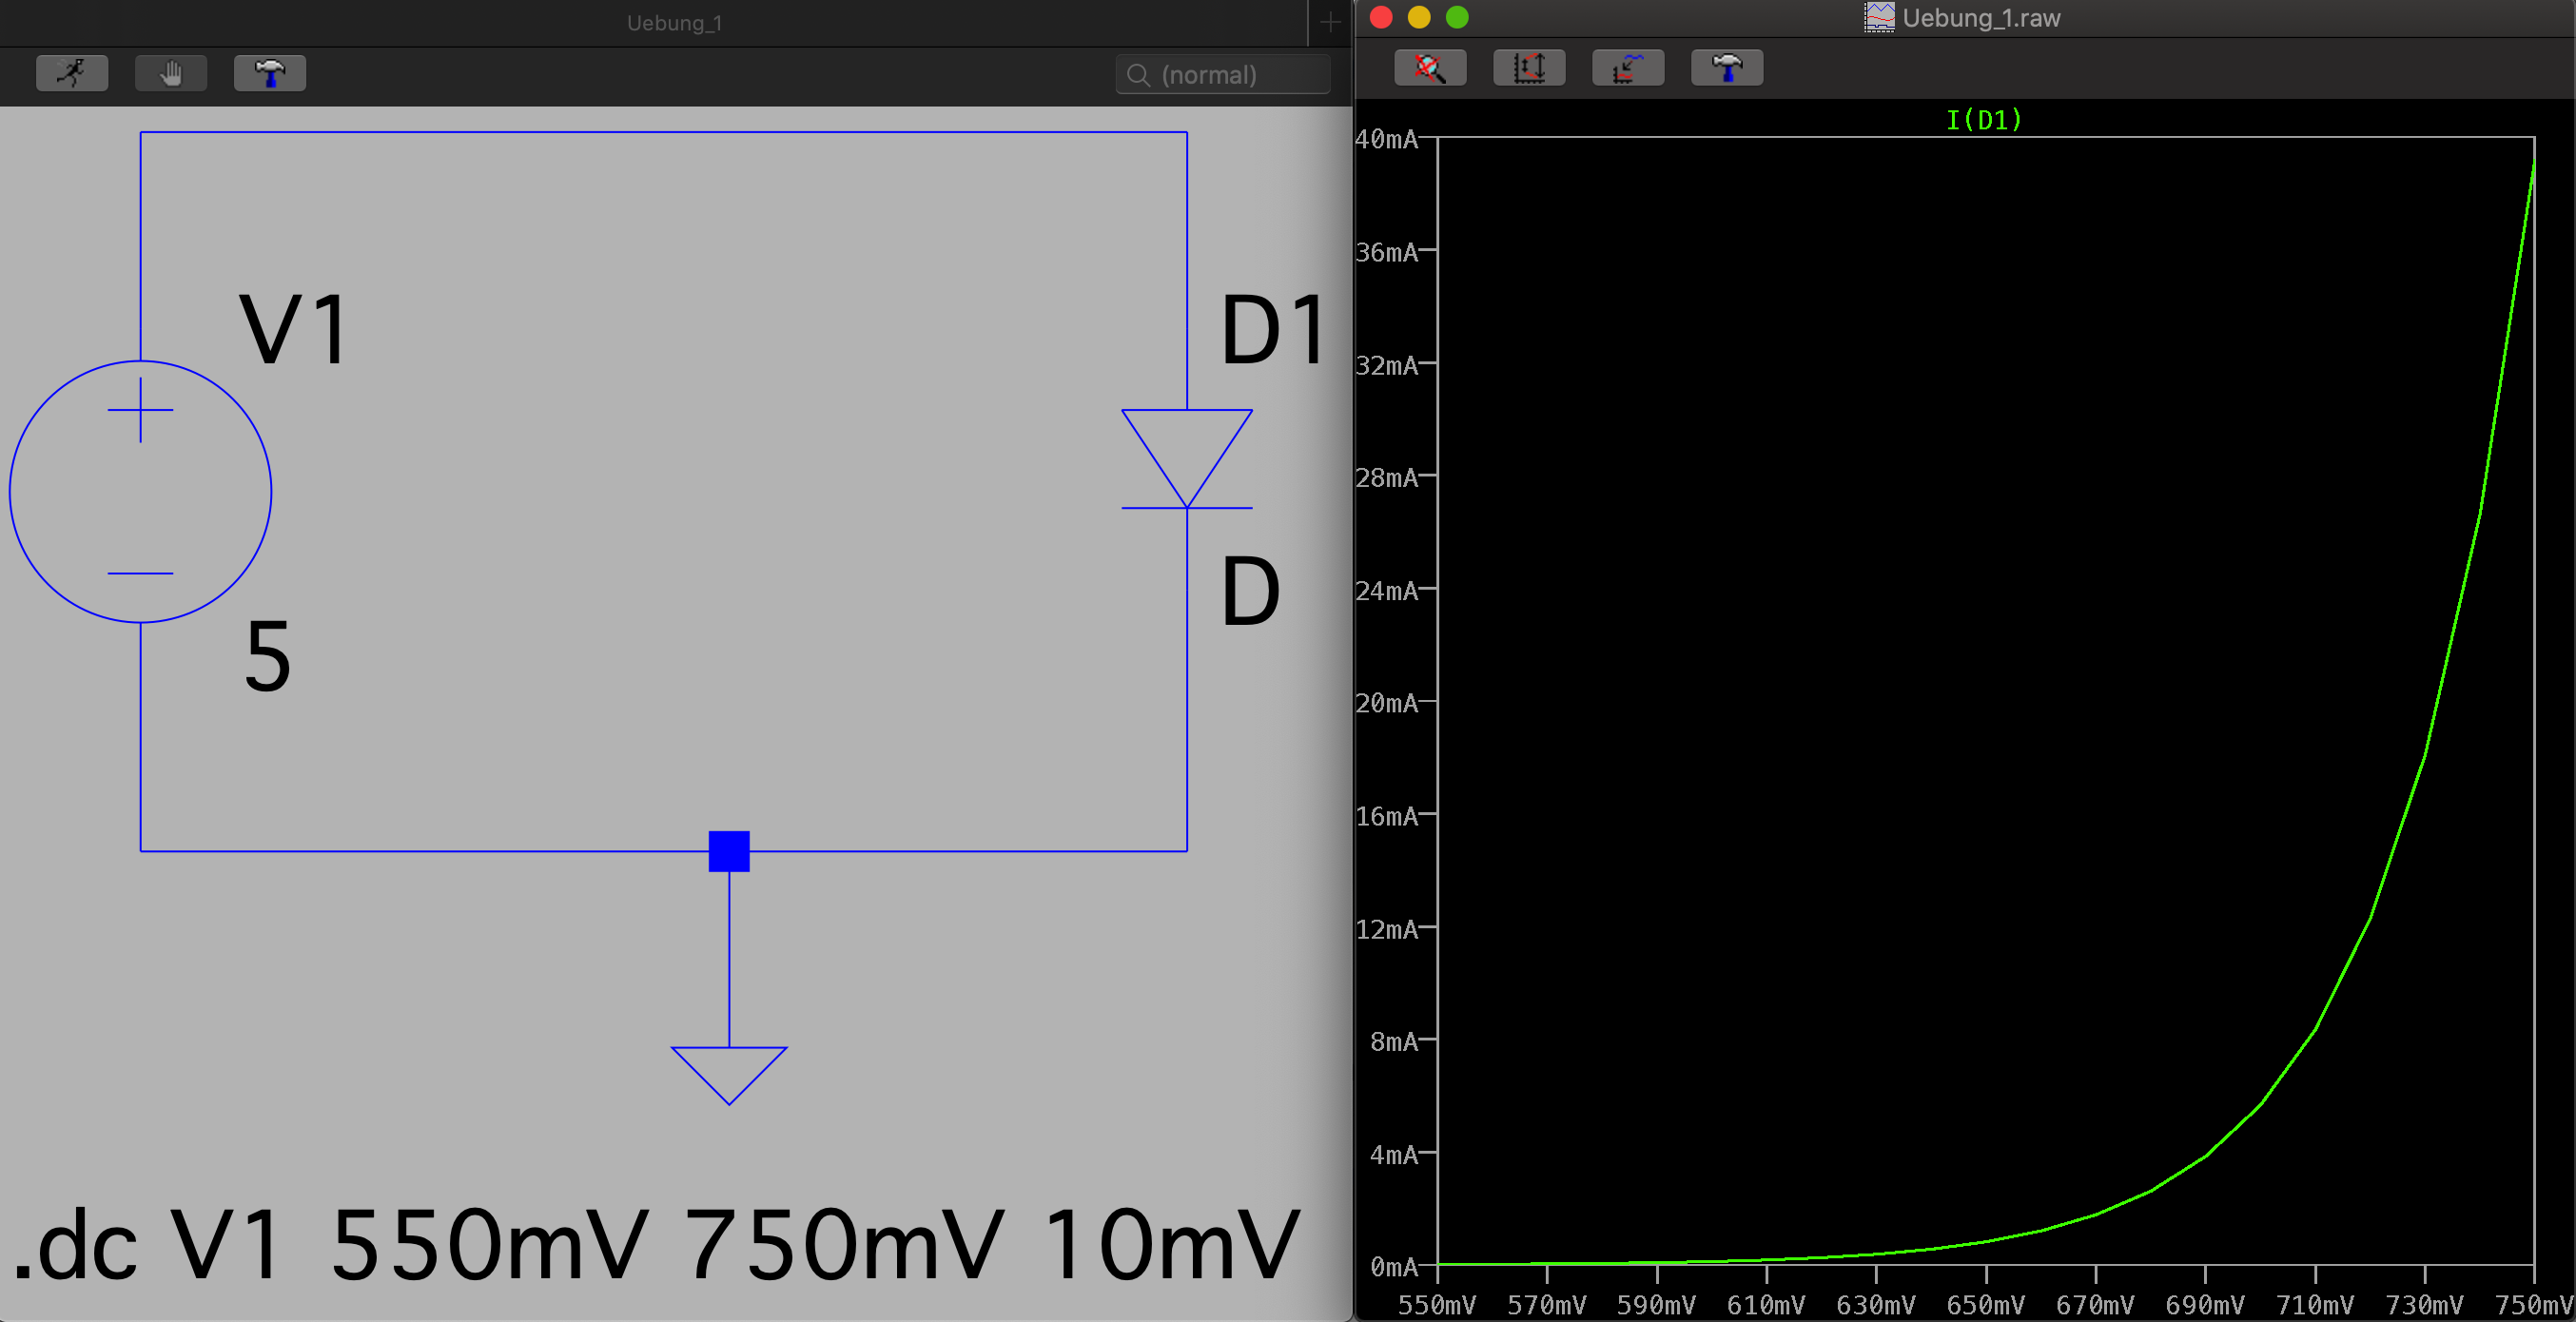
\includegraphics[width=\linewidth]{pictures/analysis_2.png}
          \end{minipage} 
          & 
          \begin{minipage}{.5\textwidth}
          \begin{itemize}
            \item Klickt auf 
\includegraphics[scale=0.3]{pictures/run.png} (run) und LTSpice startet die Simulation
          \item Wir wählen \textbf{I(D1)}, den Strom durch die Diode.
          \end{itemize}
          \end{minipage} 
          \\
        \end{tabular}
      \end{table}
    \end{tiny} \end{spacing}
    
      \begin{spacing}{0.9} \begin{tiny}
        \begin{table}[h!]
          \begin{tabular}{p{10cm} }
            \hline
            \textbf{Ergebnis und Auswertung} \\
            \hline \\    
            Wie zu erwarten liefert dieses einfache Beispiel den Zusammenhang zwischen Strom, Spannung und Wiederstand. Probiert den Spannungsbereich des
            DC-Sweep von 550 - 750 mV auf 550 mV - 2V zu erhöhen.          
            \begin{itemize}
              \item Was fällt euch auf?
              \item Könnt ihr euch herleiten, warum man eine 
              Diode immer mit einem Vorwiederstand betreiben sollte? 
            \end{itemize}  
            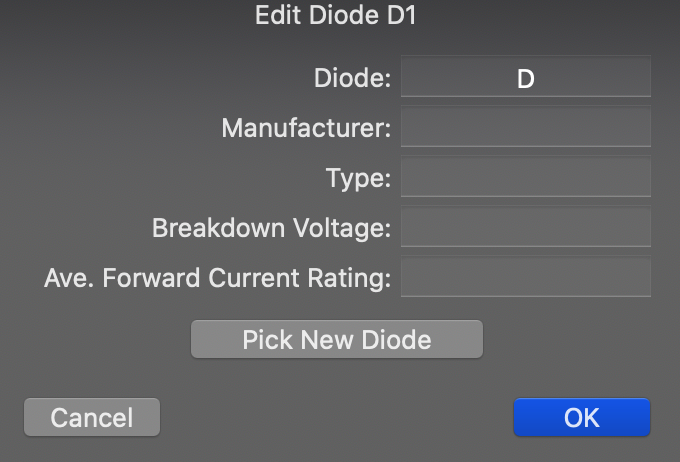
\includegraphics[scale=0.1]{pictures/diode_choice.png} \newline
            Mit einem rechten Mausklick auf die Diode könnte ihr die Dioden Typen variieren. (\textbf{pick new diode})
            Zum Beispiel von einer idealen aus dem obigen Beispiel zu einer beliebigen realen entsprechend dem Modell des Herstellers, schaut euch die Unterschiede an.
          \end{tabular}
        \end{table}
      \end{tiny} \end{spacing}
      
       \end{frame}%diode
\begin{frame}[t]{NPN-Transistor}

  \textbf{Ziel - Darstellung des Ausgangskennlinienfeld}

  \begin{spacing}{0.6} \begin{tiny}

      Das Ausgangskennlinienfeld eines npn Transistors beschreibt den Zusammenhang von Kollektorstrom $I_c$ und der Spannung
      an der Kollektor-Emitter Strecke $U_{ce}$. Das Kennlinienfeld wird für verschiedene Basisströme $I_b$ angegeben.
    \end{tiny} \end{spacing}
  \begin{spacing}{0.9} \begin{tiny}
      \begin{table}[h!]
        \begin{tabular}{p{3cm} p{7cm}}
          \hline
          \textbf{Erstellung des Schaltplans}   & \\
          \hline                                  \\
          \begin{minipage}{.3\textwidth}
            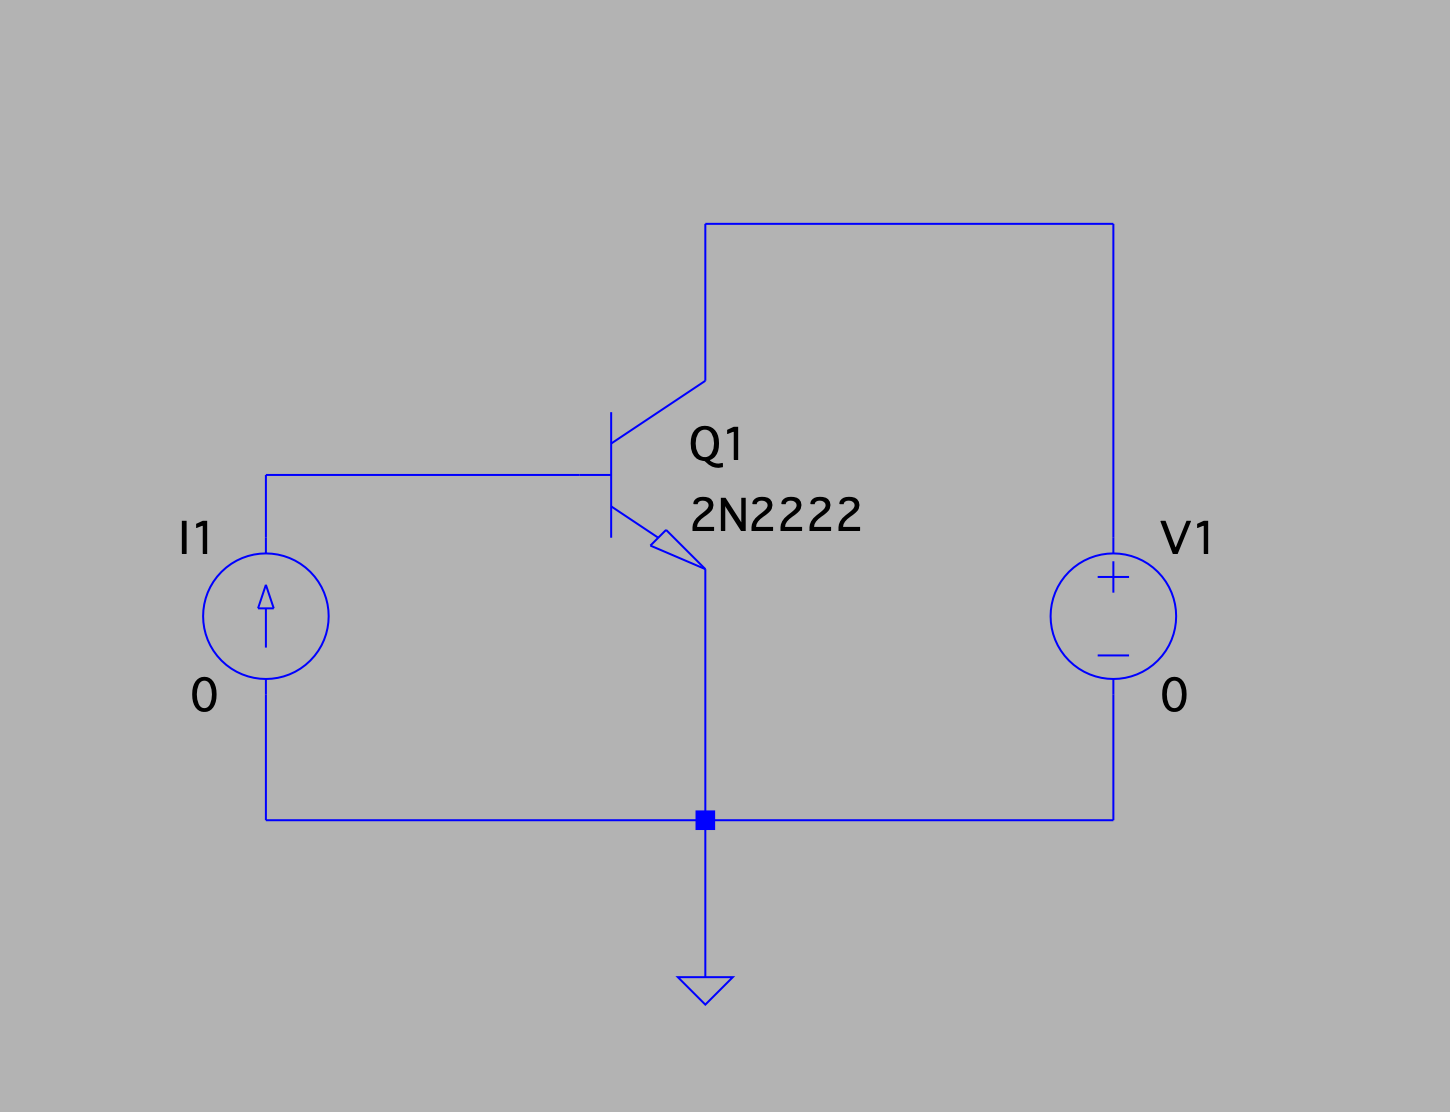
\includegraphics[width=\linewidth]{pictures/tran.png}
          \end{minipage}
                                                &
          \begin{minipage}{.7\textwidth}
            \begin{itemize}
              \item Startet mit einem neuen schematic
              \item Speichert das Projekt direkt als neue Datei ab (File $->$ save as )
              \item Fügt eine ideale Stromquelle (\textbf{F2} \dots current) hinzu und dreht dieser (\textbf{STRG+R})
              \item Fügt einen npn-Transistor(\textbf{F2} \dots npn) hinzu.
              \item Per rechtem Mausklick könnt ihr vom idealen npn anlaog zur Diode im letzten Beispiel zum 2N2222 wechseln.
              \item Verdrahtet die Schaltung wieder vollstänndig (\textbf{F3})
            \end{itemize}
          \end{minipage}
          \\
                                                & \\
          \hline
          \textbf{Konfiguration der Simulation} & \\
          \hline                                  \\
          \begin{minipage}{.3\textwidth}
            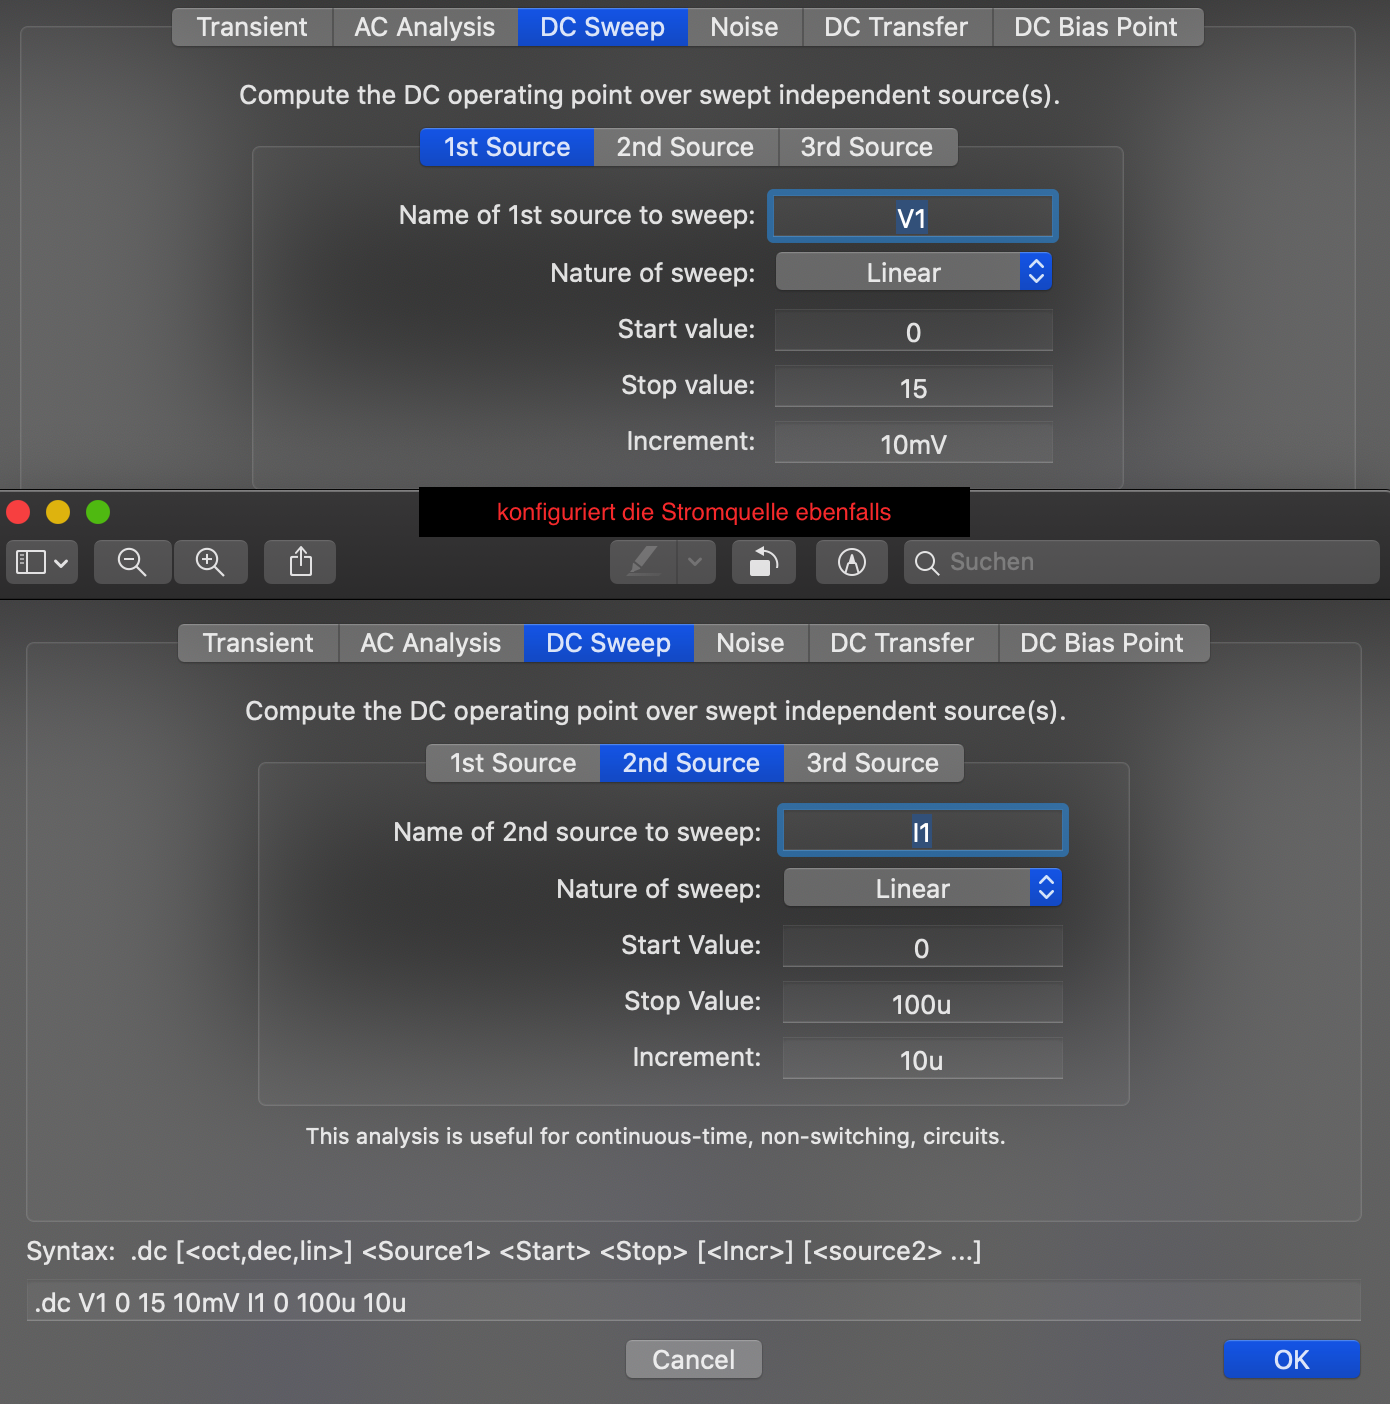
\includegraphics[width=0.8\linewidth]{pictures/simulationcmd_3.png}
          \end{minipage}
                                                &
          \begin{minipage}{.7\textwidth}
            \begin{itemize}
              \item Im Menu Simulation, wählt \textbf{Edit simulation command} und bliebt beim DC Sweep.
              \item Unser Ziel ist es das Ausgangskennlinienfeld des 2N2222 simlativ zu bestimmen. Dazu verwenden wir einen DC-Sweep
                    mit einer ideal Stromquelle (I1) die verschiedene Basisströme $I_b$ simuliert und eine Spannungsquelle (V1) die die Spannung
                    $U_{ce}$ simuliert.
              \item V1 soll von 0 - 15V in 10mV Schritten simuliert werden, I1 von 0 - 100u in 10u Schritten.
              \item Bestätigt mit \textit{OK} und fügt die Simlationsansweisung dem schematic hinzu
            \end{itemize}
          \end{minipage}
          \\
                                                & \\
          \hline
        \end{tabular}

      \end{table}

    \end{tiny} \end{spacing}

\end{frame}

\begin{frame}[t]{NPN-Transistor}

  \begin{spacing}{0.9} \begin{tiny}
      \begin{table}[h!]
        \begin{tabular}{p{5cm} p{5cm}}
          \hline
          \textbf{Simulation und Analyse} & \\
          \hline                            \\
          \begin{minipage}{.5\textwidth}
            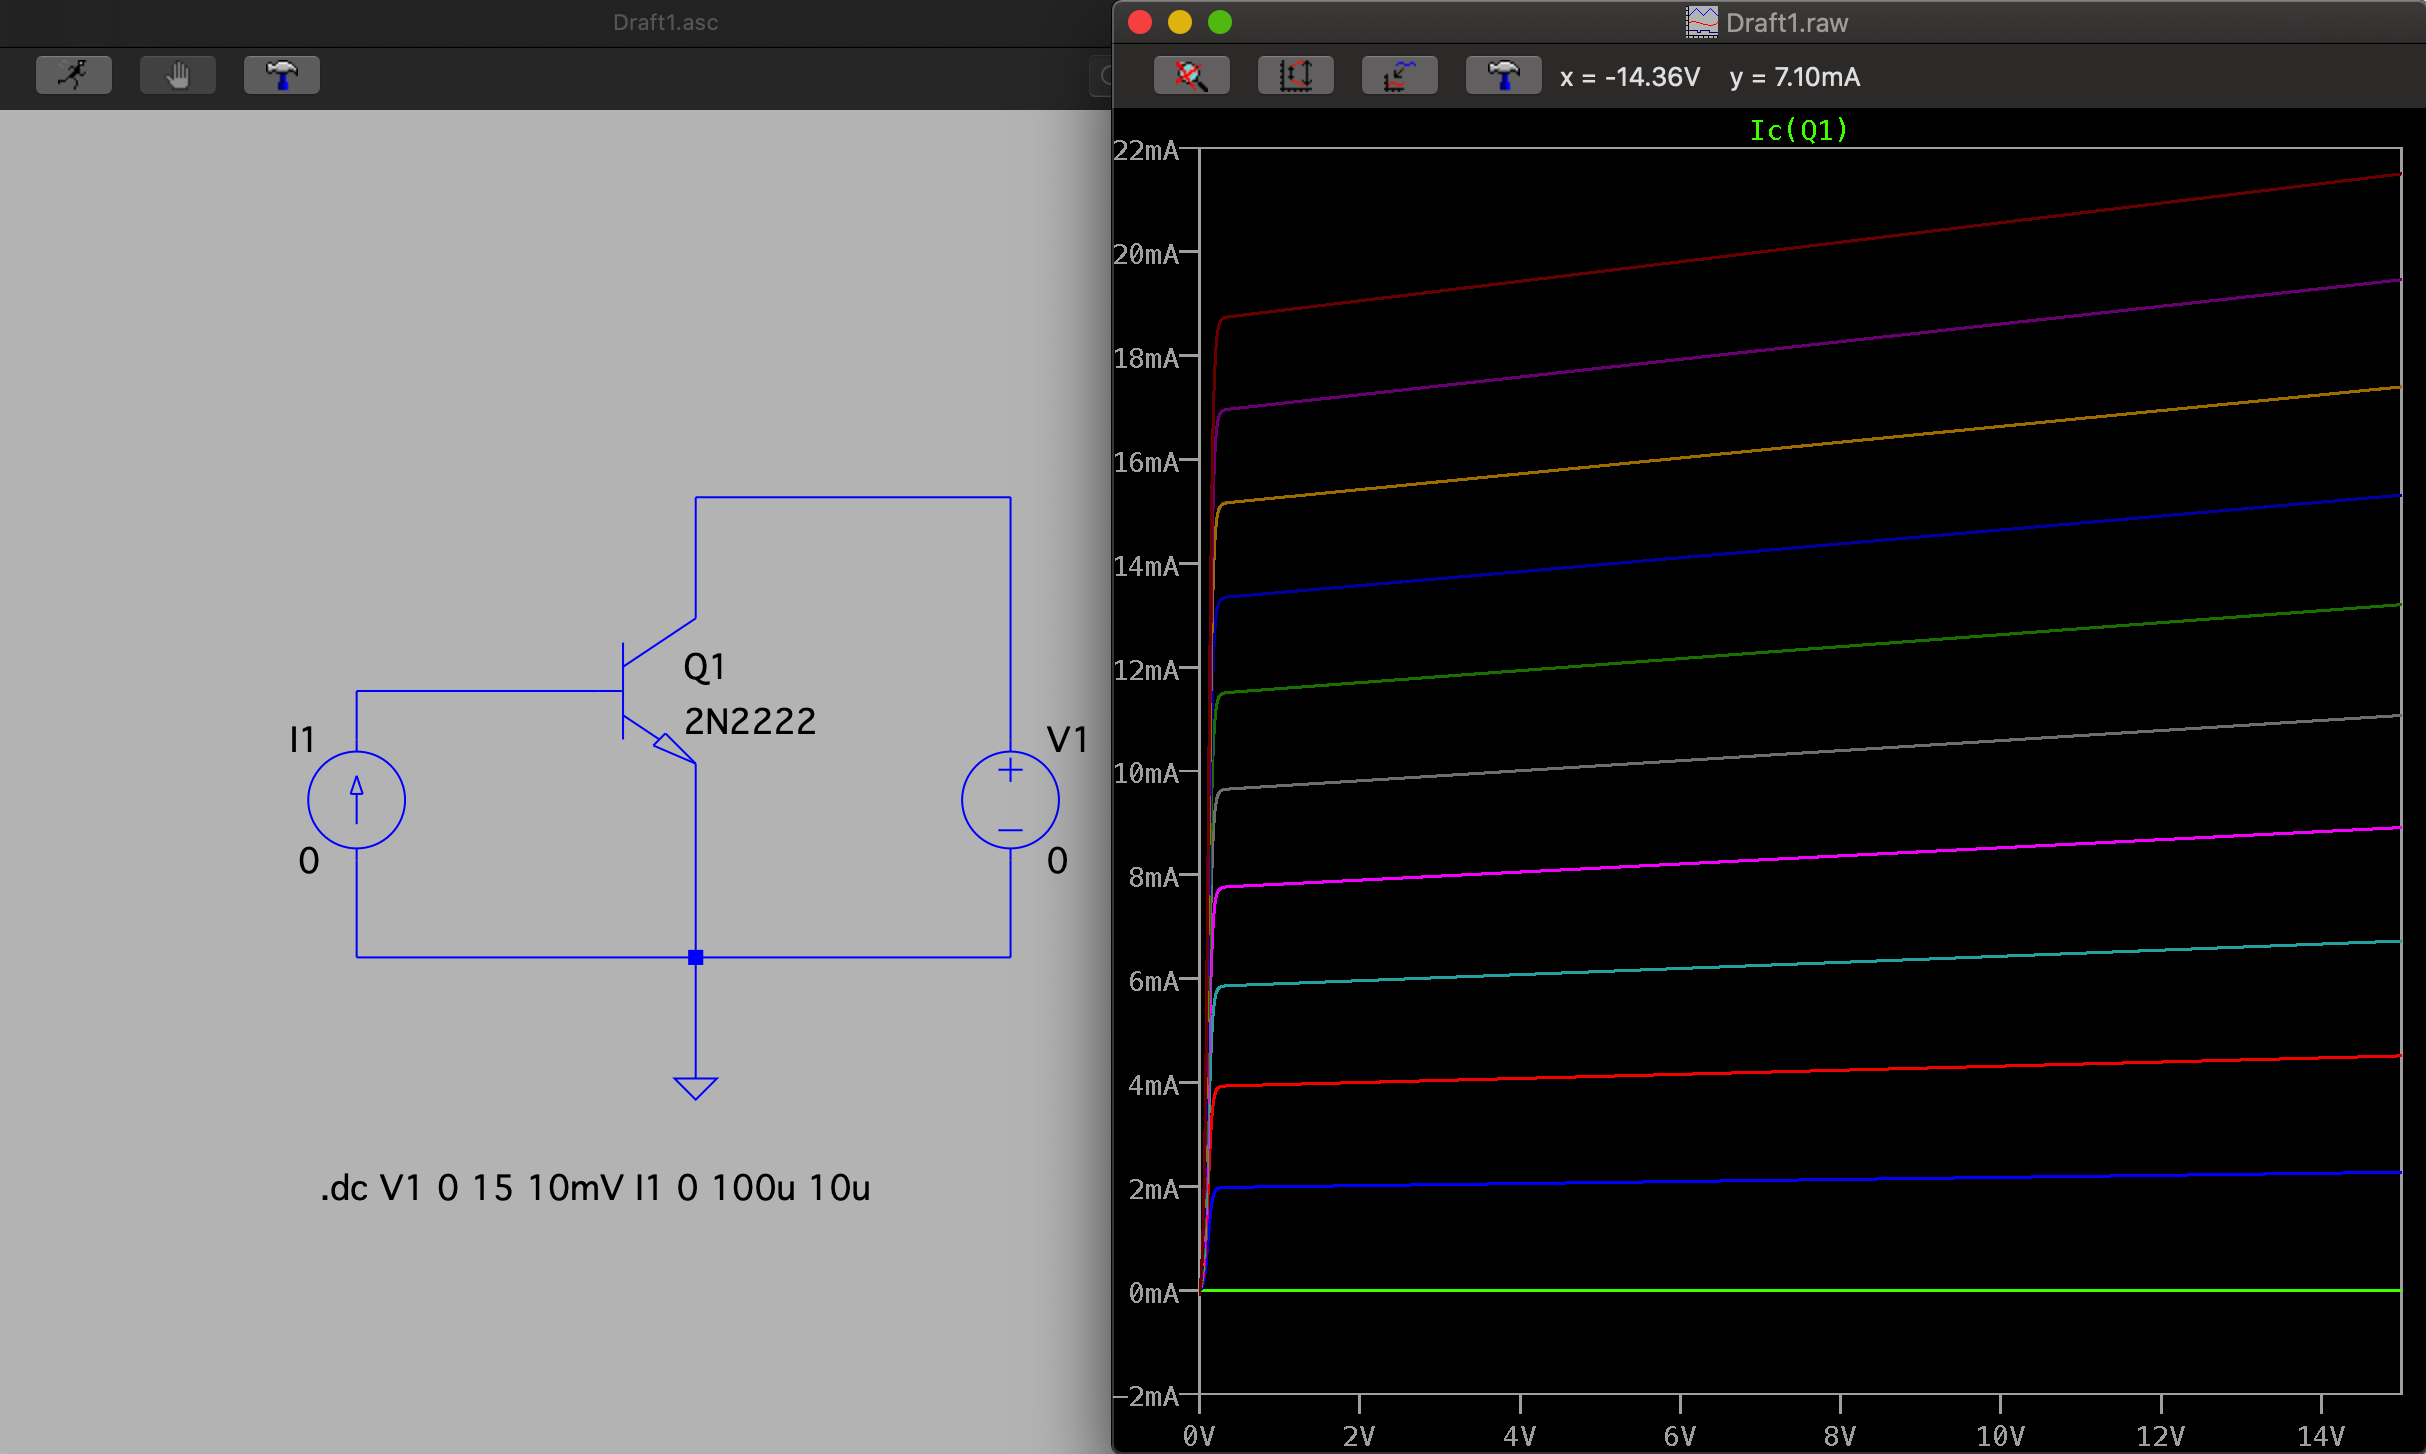
\includegraphics[width=\linewidth]{pictures/analysis_3.png}
          \end{minipage}
                                          &
          \begin{minipage}{.5\textwidth}
            \begin{itemize}
              \item Klickt auf 
\includegraphics[scale=0.3]{pictures/run.png} (run) und LTspice startet die Simulation
              \item Wir wählen \textbf{IC(Q1)}, den Kollektorstrom.
            \end{itemize}
          \end{minipage}
          \\
        \end{tabular}
      \end{table}
    \end{tiny} \end{spacing}

  \begin{spacing}{0.9} \begin{tiny}
      \begin{table}[h!]
        \begin{tabular}{p{10cm} }
          \hline
          \textbf{Ergebnis und Auswertung} \\
          \hline                           \\
          Jeder Graph steht für einen simulierten Basisstrom. Per rechtem Mausklick $->$ View $->$ Steps könnt ihr einzelne Graphen zur
          detaillierten Analyse auswählen. \newline\newline Achtet darauf, welche Quelle ihr im $.dc ...$ simulation command zuerst wählt. \textbf{Quelle 1 ergibt im Diagramm die Abszisse, die Quelle 2 die Ordinate.}
        \end{tabular}
      \end{table}
    \end{tiny} \end{spacing}

\end{frame}

\begin{frame}[t]{NPN-Transistor}

  \begin{spacing}{0.6} \begin{tiny}

      Wenn ihr den Zusammenhang zwischen der Basisspannung $U_{be}$ und dem Kollektorstrom $I_c$ simulativ herausfinden wollt, müsst
      ihr die Schaltung leicht variieren. Dazu werden wir das schematic wie folgt anpassen.

    \end{tiny} \end{spacing}
  \begin{spacing}{0.9} \begin{tiny}
      \begin{table}[h!]
        \begin{tabular}{p{3cm} p{7cm}}
          \hline
          \textbf{Erstellung des Schaltplans}   & \\
          \hline                                  \\
          \begin{minipage}{.3\textwidth}
            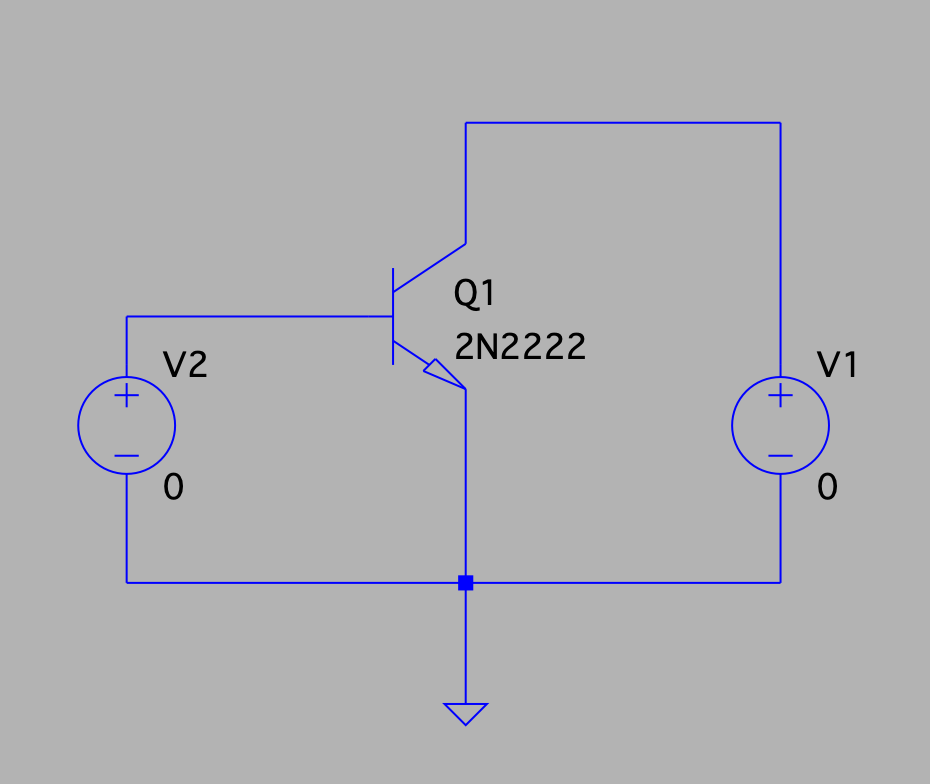
\includegraphics[width=\linewidth]{pictures/tran2.png}
          \end{minipage}
                                                &
          \begin{minipage}{.7\textwidth}
            \begin{itemize}
              \item Speichert das Projekt direkt als neue Datei ab (File $->$ save as )
              \item Löscht die Stromquelle (\textbf{F5}) und fügt eine Spannungsquelle hinzu.
              \item Verdrahtet die Schaltung wieder vollstänndig (\textbf{F3})
              \item Super simple dieses mal :)
            \end{itemize}
          \end{minipage}
          \\
                                                & \\
          \hline
          \textbf{Konfiguration der Simulation} & \\
          \hline                                  \\
          \begin{minipage}{.3\textwidth}
            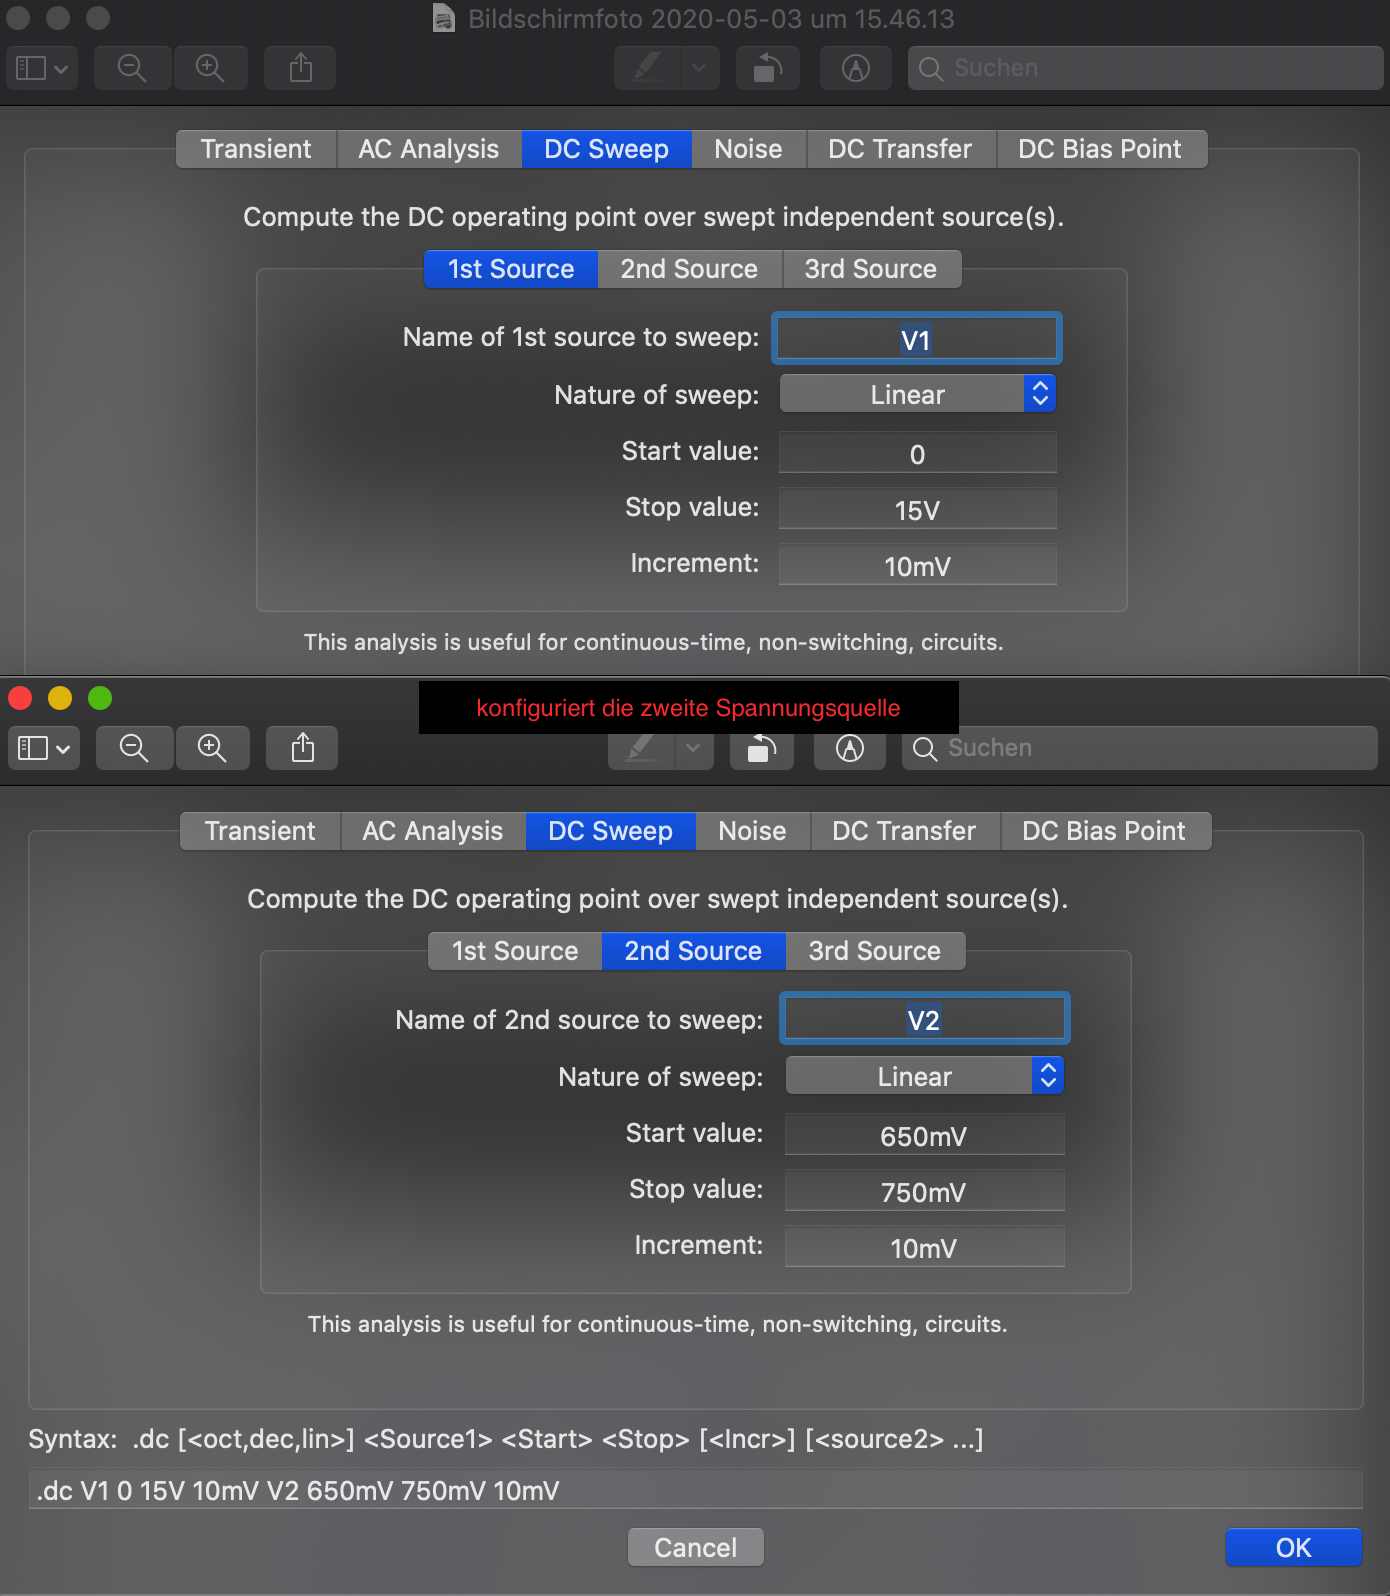
\includegraphics[width=0.8\linewidth]{pictures/simulationcmd_4.png}
          \end{minipage}
                                                &
          \begin{minipage}{.7\textwidth}
            \begin{itemize}
              \item Im Menu Simulation, wählt \textbf{Edit simulation command} und bliebt beim DC Sweep.
              \item Unser Ziel ist es das Ausgangskennlinienfeld des 2N2222 simlativ zu bestimmen. Dazu verwenden wir dieses mal
                    einen DC-Sweep mit einer Spannungsquelle, die die Basis-Emitterspannung $U_{be}$ simuliert und eine Spannungsquelle (V1) die die Spannung
                    $U_{ce}$ simuliert.
              \item V1 soll von 0 - 15V in 10mV Schritten simuliert werden, V2 von 650 - 750 mV in 10mV Schritten.
              \item Bestätigt mit \textit{OK} und fügt die Simlationsansweisung dem schematic hinzu
            \end{itemize}
          \end{minipage}
          \\
                                                & \\
          \hline
        \end{tabular}

      \end{table}

    \end{tiny} \end{spacing}

\end{frame}



\begin{frame}[t]{NPN-Transistor}

  \begin{spacing}{0.9} \begin{tiny}
      \begin{table}[h!]
        \begin{tabular}{p{5cm} p{5cm}}
          \hline
          \textbf{Simulation und Analyse} & \\
          \hline                            \\
          \begin{minipage}{.5\textwidth}
            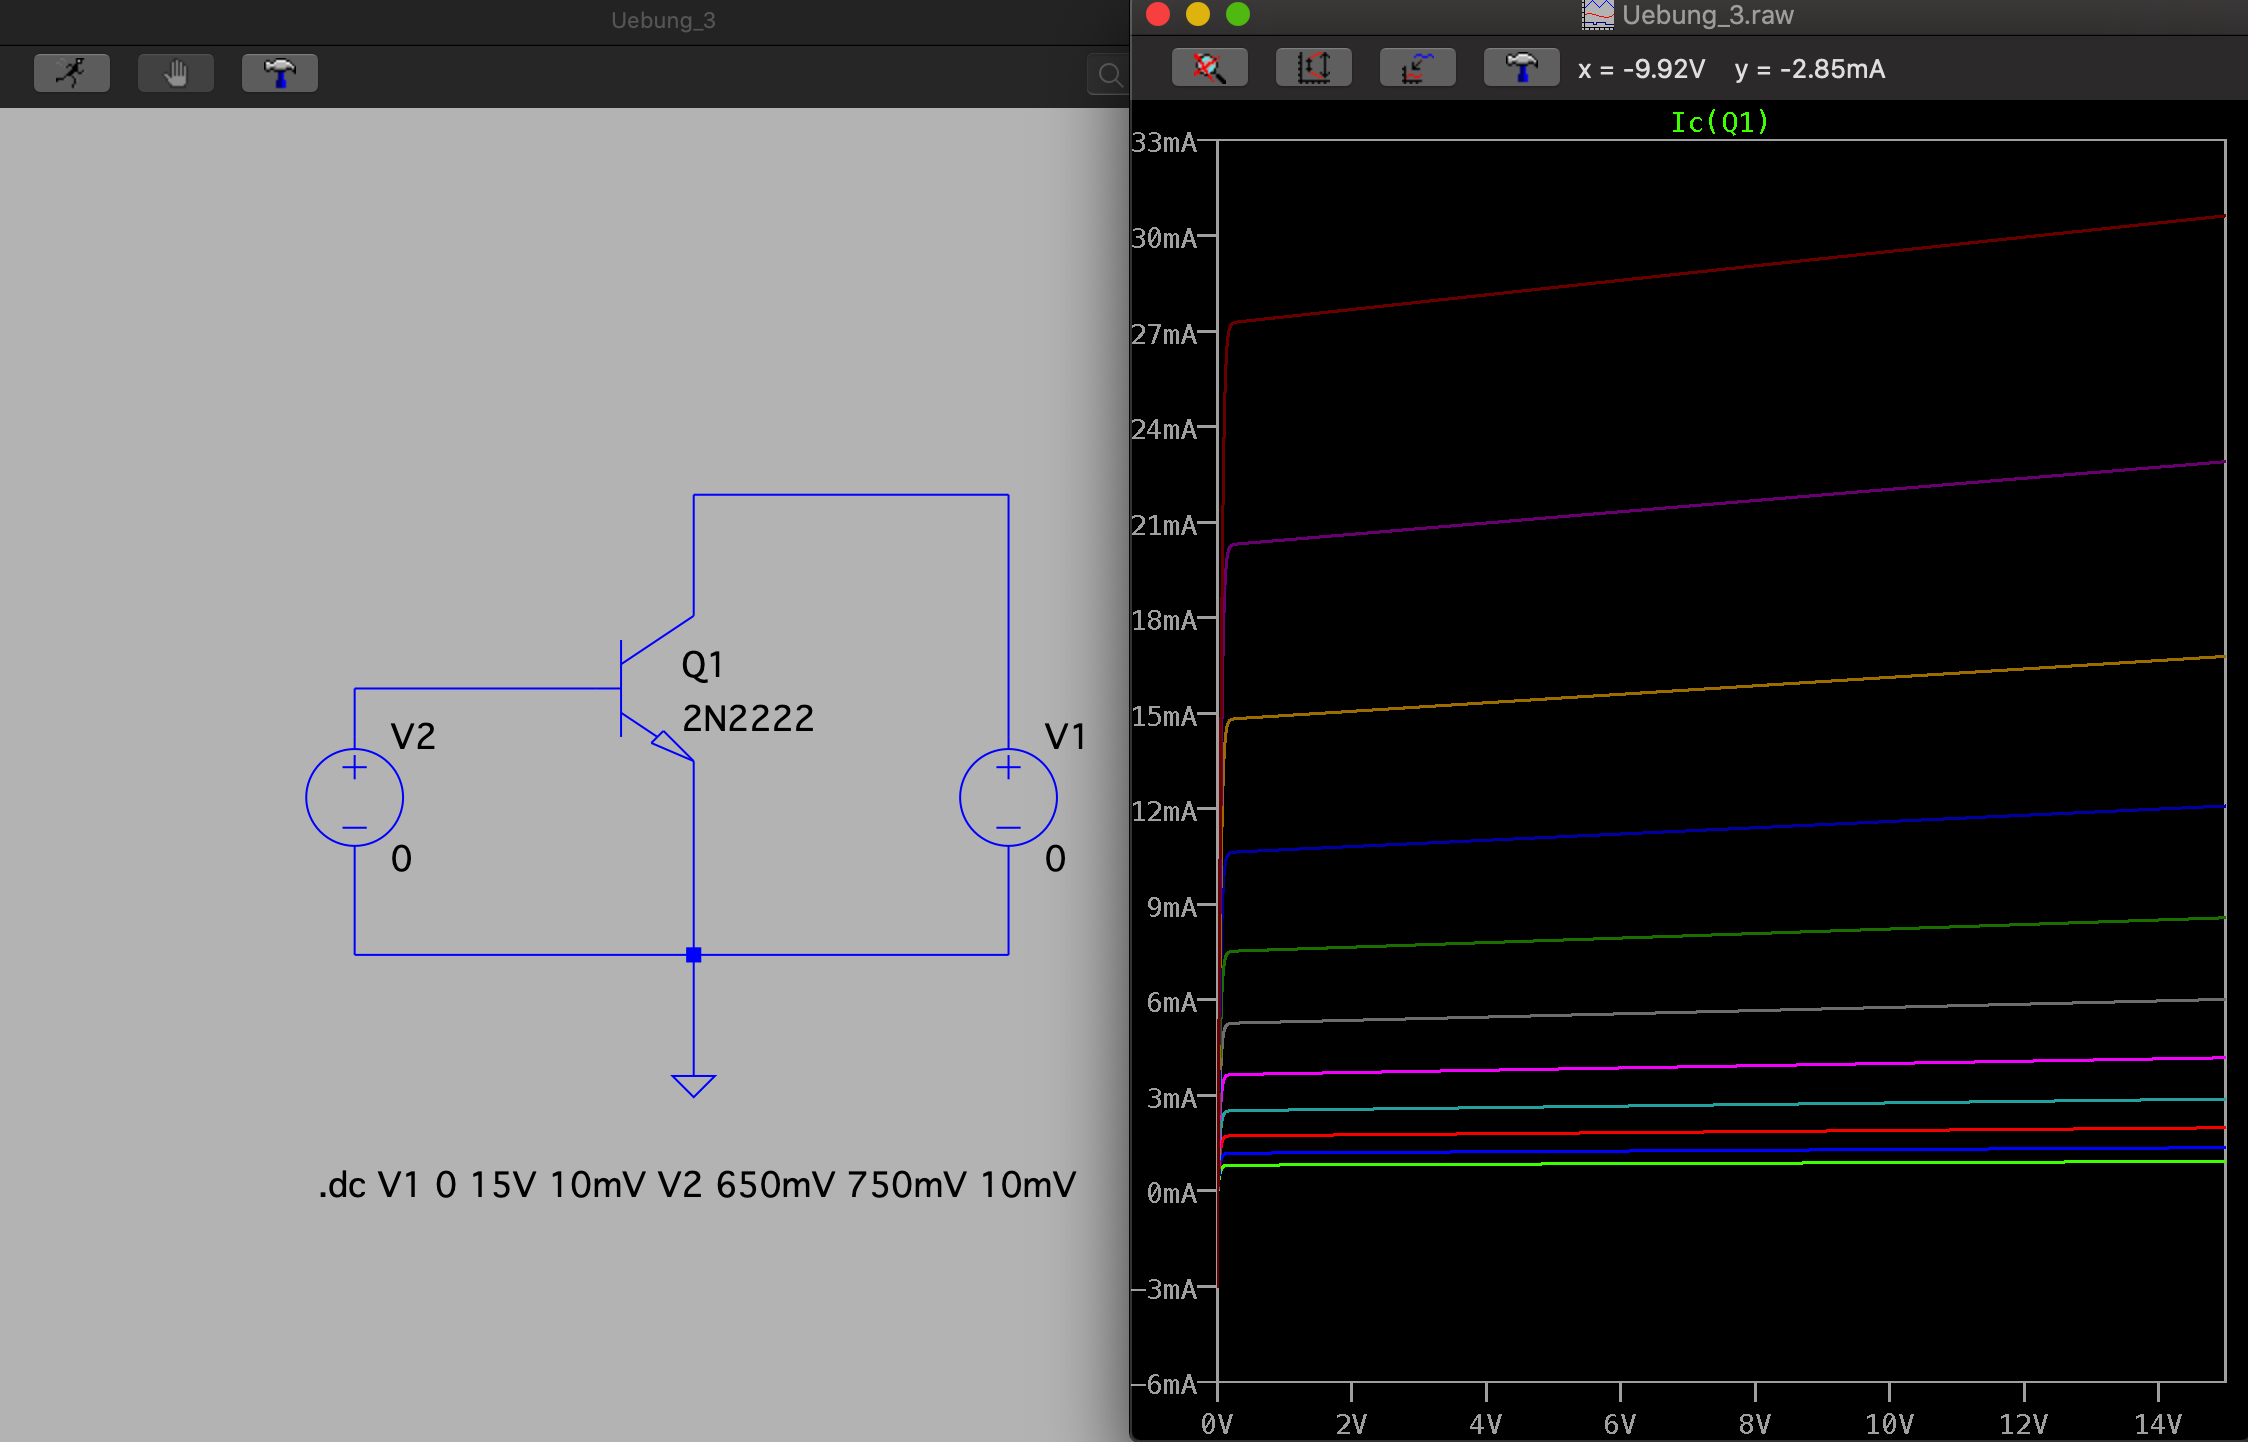
\includegraphics[width=\linewidth]{pictures/analysis_4.png}
          \end{minipage}
                                          &
          \begin{minipage}{.5\textwidth}
            \begin{itemize}
              \item Klickt auf 
\includegraphics[scale=0.3]{pictures/run.png} (run) und LTspice startet die Simulation
              \item Wir wählen \textbf{IC(Q1)}, den Kollektorstrom.
            \end{itemize}
          \end{minipage}
          \\
        \end{tabular}
      \end{table}
    \end{tiny} \end{spacing}

  \begin{spacing}{0.9} \begin{tiny}
      \begin{table}[h!]
        \begin{tabular}{p{10cm} }
          \hline
          \textbf{Ergebnis und Auswertung} \\
          \hline                           \\
          Jeder Graph steht für eine simulierte $U_{be}$. Per rechtem Mausklick $->$ View $->$ Steps könnt ihr einzelne Graphen zur
          detaillierten Analyse auswählen. \newline\newline Achtet darauf, welche Quelle ihr im $.dc ...$ simulation command zuerst wählt. \textbf{Quelle 1 ergibt im Diagramm die Abszisse, die Quelle 2 die Ordinate.}
        \end{tabular}
      \end{table}
    \end{tiny} \end{spacing}

\end{frame}%transistor
\begin{frame}[t]{OPV Schaltungen - transient, ideal}

    \textbf{Ziel - Simulation eines invertierenden Verstärkers}
    
    \begin{spacing}{0.6} \begin{tiny}
    
    Wir wollen in einem einfachen simulativen Experiment die Funktionalität eines invertierenden Verstärkers nachvollziehen. 
    \begin{spacing}{0.9} \begin{tiny}
      \begin{table}[h!]
        \begin{tabular}{p{5cm} p{5cm}}
          \begin{minipage}{.5\textwidth}
            \begin{figure}
              \scalebox{0.35}{
            \centering
            \begin{circuitikz}
              \ctikzset{bipoles/length=1cm}
              \draw
              (0, 0) node[op amp] (opamp) {}
              (opamp.-) to[R,l_=$R_1$,-o] (-2, 0.35) -- (-3, 0.35) to [V=$v_1$] (-3,-0.5) to (-3,-0.5) node[ground]{}
              (opamp.-) to[short,*-] ++(0,0.5) coordinate (leftC)
              to[R=$R_2$] (leftC -| opamp.out)
              to[short,-*] (opamp.out) to [short,-o] (1.5,0) to (1.5,-0.5) node[ground]{}
              (opamp.+) -- (-1,-0.35) to (-1,-0.5) node[ground]{}
              ;
            \end{circuitikz}
              }
          \end{figure}
          \end{minipage} 
          & 
          \begin{minipage}{.5\textwidth}
          \begin{equation}
            V_{out}=-\frac{R2}{R1}V_{1}
            \end{equation}
          \end{minipage} 
        \end{tabular}
      
      \end{table}
      
      \end{tiny} \end{spacing}


  Wenn man nur daran interessiert ist die grundsätzliche Funktionalität einer Schaltung zu verifizieren, kann man ideale
  Bauelemente aus der LTspice Bibliothek verwenden. Wie im obigen Beispiel benötigt z.B. der Operationsverstärker entgegen der Realität dann keine Spannungsversorgung.
  Für einen idealen OPV bietet LTspice das Bauelement \textbf{opamp} an, welches Ihr im Bauteileditor findet direkt über die Suche findet. \newline
  \textbf{Wichtig:} Ihr müsst als Spice-Direktive jedoch noch ein zu verwendendes Model einbinden. (.lib opamp.sub)
    \end{tiny} \end{spacing}
    \begin{spacing}{0.9} \begin{tiny}
    \begin{table}[h!]
      \begin{tabular}{p{3cm} p{7cm}}
        \hline
        \textbf{Erstellung des Schaltplans} & \\
        \hline \\
        \begin{minipage}{.3\textwidth}
          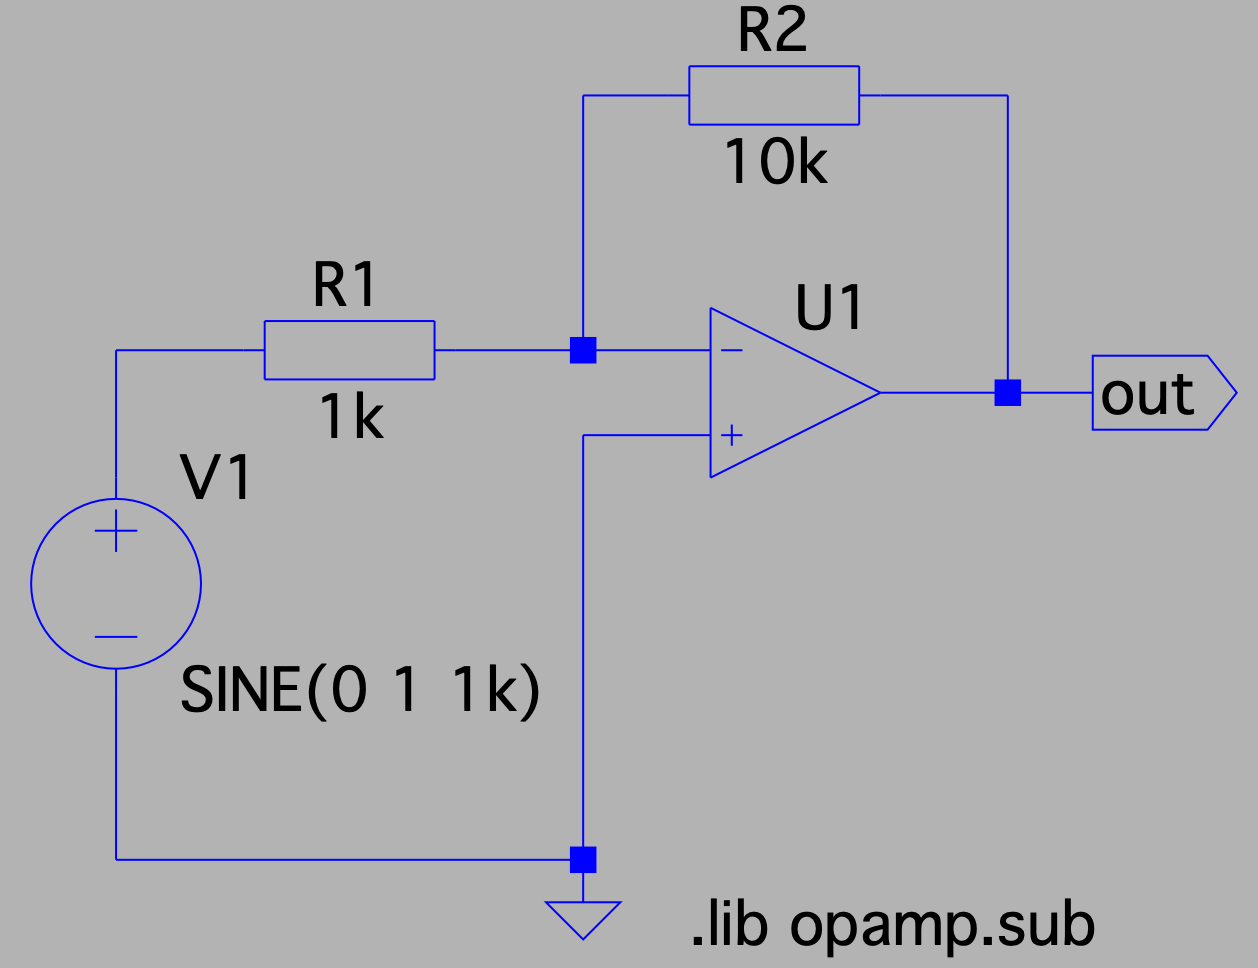
\includegraphics[width=0.8\linewidth]{pictures/opamp_1.png}
        \end{minipage} 
        & 
        \begin{minipage}{.7\textwidth}
        \begin{itemize}
          \item Baut den Schaltplan mit dem o.g. opamp als OPV auf. 
          \item Über einen rechten Mausklick kommt ihr ins \textbf{Advanced} Menü der Spannungsquelle. Hier könnt ihr Sie als Signalgenerator konfigurieren. Wir wählen einen \textbf{Sinus mit 1V Amplitude und der Frequenz 1kHz}
          \item Die library kann direkt als spice directive eingebunden werden (siehe Folie 5, .op)
          \item Ihr könnt über die Funktion \textbf{Label Net (F4)} einen Knoten umbennen und ihm mit einem Symbol für In-/Output versehen. Nennt den Ausgang der Schaltung z.B. \textit{out}.
          \item \textbf{Hinweis:} Wenn ihr einen Knoten benennt, dann kann liegt unter diesem Namen überall im Schaltplan das selbe! Potential an. 
          Dadurch könnt ihr den Plan übersichtlicher gestalten. 
        \end{itemize}
        \end{minipage} 
        \\
         & \\
         \hline
      \end{tabular}
    
    \end{table}
    
    \end{tiny} \end{spacing}
    
     \end{frame}
    
     \begin{frame}[t]{OPV Schaltungen - transient, ideal}
    
      \begin{spacing}{0.9} \begin{tiny}
      \begin{table}[h!]
        \begin{tabular}{p{4cm} p{6cm}}
          \hline
          \textbf{Konfiguration der Simulation} & \\
          \hline \\
          \begin{minipage}{.3\textwidth}
           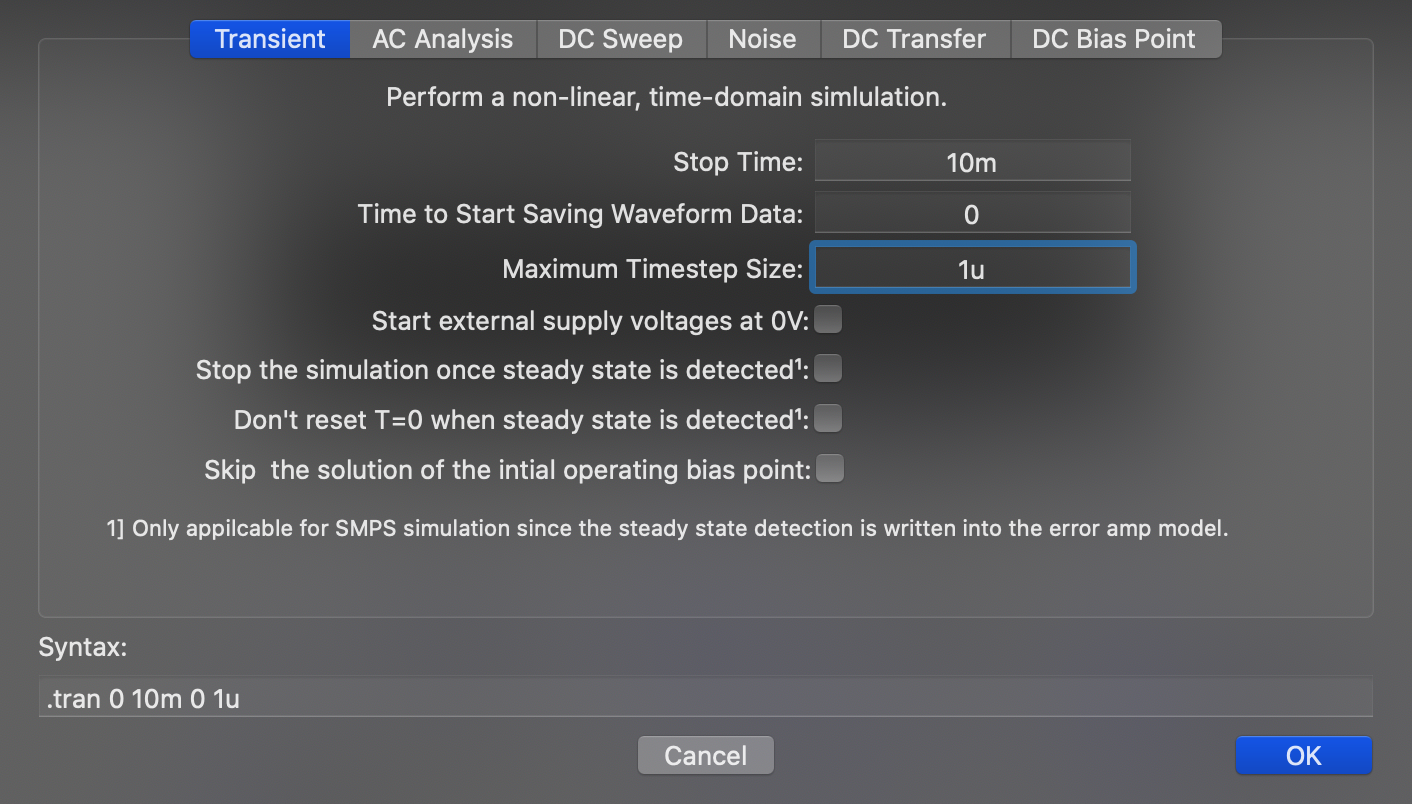
\includegraphics[width=\linewidth]{pictures/simulationcmd_5.png}
         \end{minipage} 
         & 
         \begin{minipage}{.7\textwidth}
         \begin{itemize}
           \item Im Menu Simulation, wählt \textbf{Edit simulation command} und wählt eine \textbf{Transient} Analyse. 
           \item Unser Ziel ist es am Ausgang eine Verstärkte Spannung entsprechend des Verstärkungsfaktors der Schaltung zu messen.
           \item Da die Schaltung ideal kein Einschwingverhalten zeigt, starten wir direkt mit der Aufzeichnung und simulieren 10ms mit einer Schrittweite von 10us.
           \item Bestätigt mit \textit{OK} und fügt die Sumlationsansweisung dem schematic hinzu
         \end{itemize}
         \end{minipage} 
         \\
          & \\
          \hline
          \textbf{Simulation und Analyse} & \\
          \hline \\
          \begin{minipage}{.5\textwidth}
            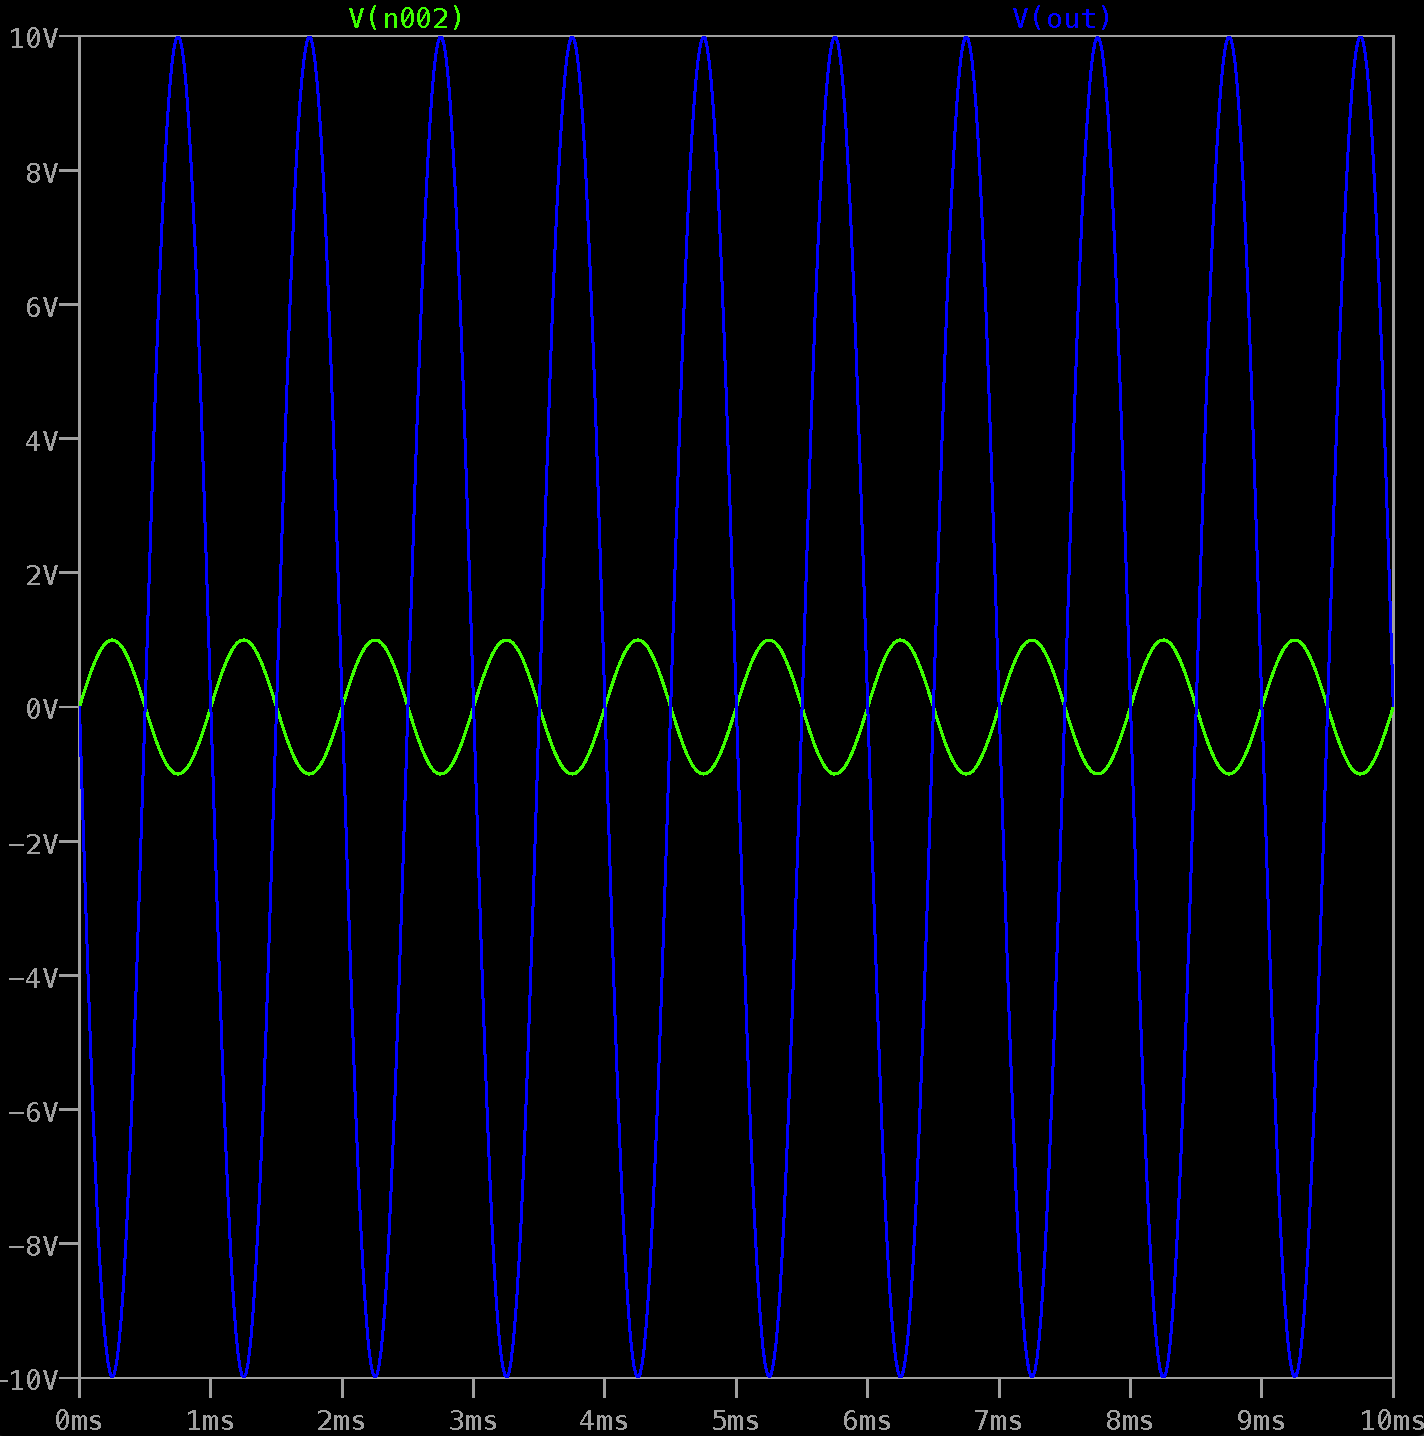
\includegraphics[width=0.5\linewidth]{pictures/analysis_5.png}
          \end{minipage} 
          & 
          \begin{minipage}{.5\textwidth}
          \begin{itemize}
            \item Klickt auf 
\includegraphics[scale=0.3]{pictures/run.png} (run) und LTspice startet die Simulation
            \item Fügt nun die Eingangsspannung sowie die Ausgangsspannung der Schaltung als Messpunkte hinzu.
          \end{itemize}
          \end{minipage} 
          \\
        \end{tabular}
      \end{table}
    \end{tiny} \end{spacing}
    
      \begin{spacing}{0.9} \begin{tiny}
        \begin{table}[h!]
          \begin{tabular}{p{10cm} }
            \hline
            \textbf{Ergebnis und Auswertung} \\
            \hline \\    
            Verifiziert, ob die Verstärkung sowie das invertierende Verhalten zu eurem Erwartungswert (10) passt. 
          \end{tabular}
        \end{table}
      \end{tiny} \end{spacing}
      
       \end{frame}

       \begin{frame}[t]{OPV Schaltungen - transient, nicht ideal}

        \begin{spacing}{0.6} \begin{tiny}
        Im nächsten Experiment wollen wir die gleiche Schaltung mit einem "nicht idealen" Verstärken simulieren und die Verwendung
        von Labels verdeutlichen. 
        \end{tiny} \end{spacing}
  
        \begin{spacing}{0.9} \begin{tiny}
        \begin{table}[h!]
          \begin{tabular}{p{3cm} p{7cm}}
            \hline
            \textbf{Erstellung des Schaltplans} & \\
            \hline \\
            \begin{minipage}{.3\textwidth}
              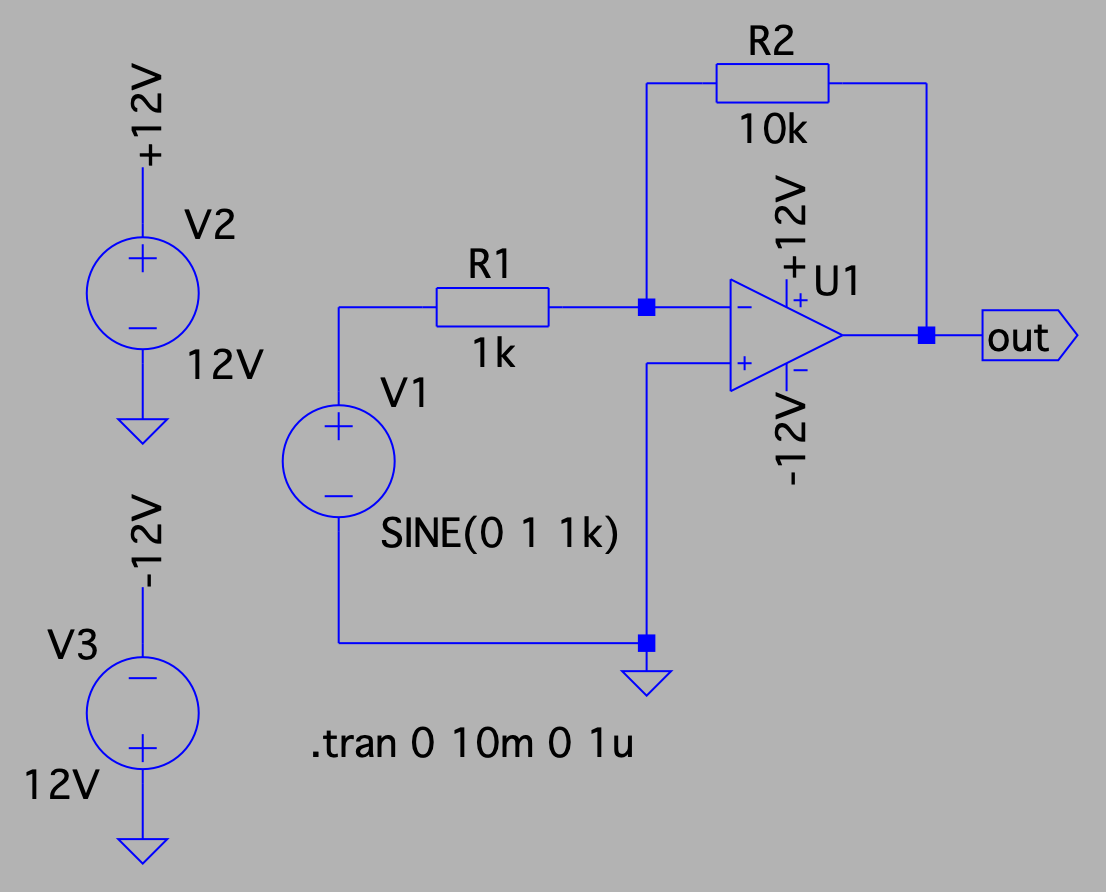
\includegraphics[width=0.8\linewidth]{pictures/opamp_2.png}
            \end{minipage} 
            & 
            \begin{minipage}{.7\textwidth}
            \begin{itemize}
              \item Tauscht den opamp gegen das Bauteil \textbf{UniversalOpamp2} aus dem Bauteileditor (\textbf{F2}).
              \item Fügt zwei neue Spannungsquellen für die Versorgung des OPV's hinzu. 
              \item Achtet hierbei auf darauf, dass die Label wirklich auf dem Potential +12V und -12V liegen.
              \item Erstellt die Labels +12V und -12V (\textbf{Label Net (F4)}).
            \end{itemize}
            \end{minipage} 
            \\
          \end{tabular}

        \end{table}
        
        \end{tiny} \end{spacing}

                    
      \begin{spacing}{0.9} \begin{tiny}
        \begin{table}[h!]
          \begin{tabular}{p{10cm} }
            \hline
            \textbf{Ergebnis und Auswertung} \\
            \hline \\    
            Es muss das selbe Ergebnis herauskommen wie im vorherigen Experiment unter Verwendung des idealen OPV's \textbf{opamp}.
          \end{tabular}
        \end{table}
      \end{tiny} \end{spacing}
        
         \end{frame}


       \begin{frame}[t]{OPV Schaltungen - Analyse der Grenzfrequenz einer Schaltung }

        \begin{spacing}{0.6} \begin{tiny}
        Eine Kennzahl von Tief-/Hochpassfiltern ist ihre 3dB Grenzfrequenz $f_g$. Die Grenzfrequenz kann man analytisch, jedoch auch simulativ
        über LTspice bestimmen. Hierzu bietet LTspice die Möglichkeit die Frequenz einer Schaltung zu variieren. Dies wird AC-Sweep genannt. 
        Im Bode-Diagramm kann man den logarithmischen Verlauf der Amplitude über der Frequenz in LTspice darstellen und 
        somit einfach grafisch die Grenzfrequenz bestimmen indem man den Punkt heraussucht, bei dem die Amplitde um 3dB abgefallen ist.
        \end{tiny} \end{spacing}
  
        \begin{spacing}{0.9} \begin{tiny}
          \begin{table}[h!]
            \begin{tabular}{p{10cm}}
              \hline
              \textbf{Erstellung des Schaltplans + Konfiguration der Simulation} \\
              \hline     
            \end{tabular}
          \begin{tabular}{p{2cm} p{2cm} p{6cm}}
            \begin{minipage}{.2\textwidth}
              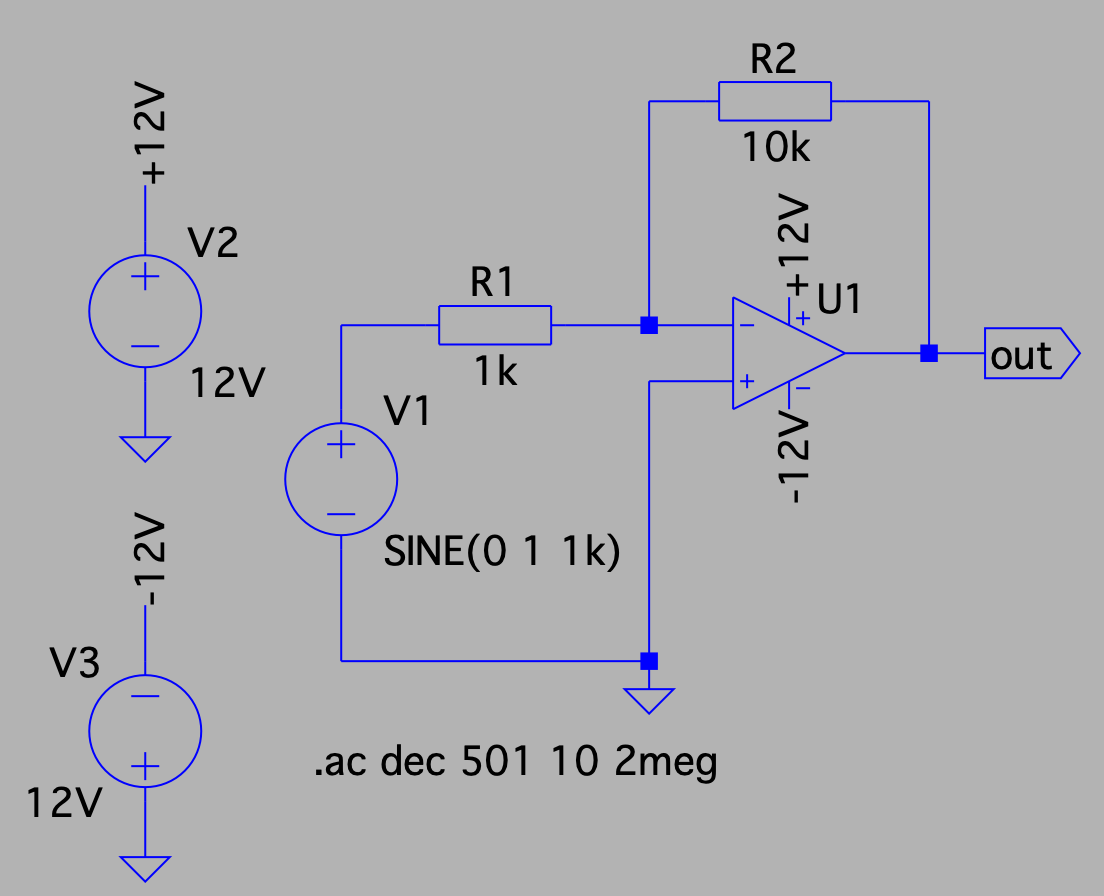
\includegraphics[width=0.8\linewidth]{pictures/opamp_3.png}
            \end{minipage} 
            &  
            \begin{minipage}{.2\textwidth}
              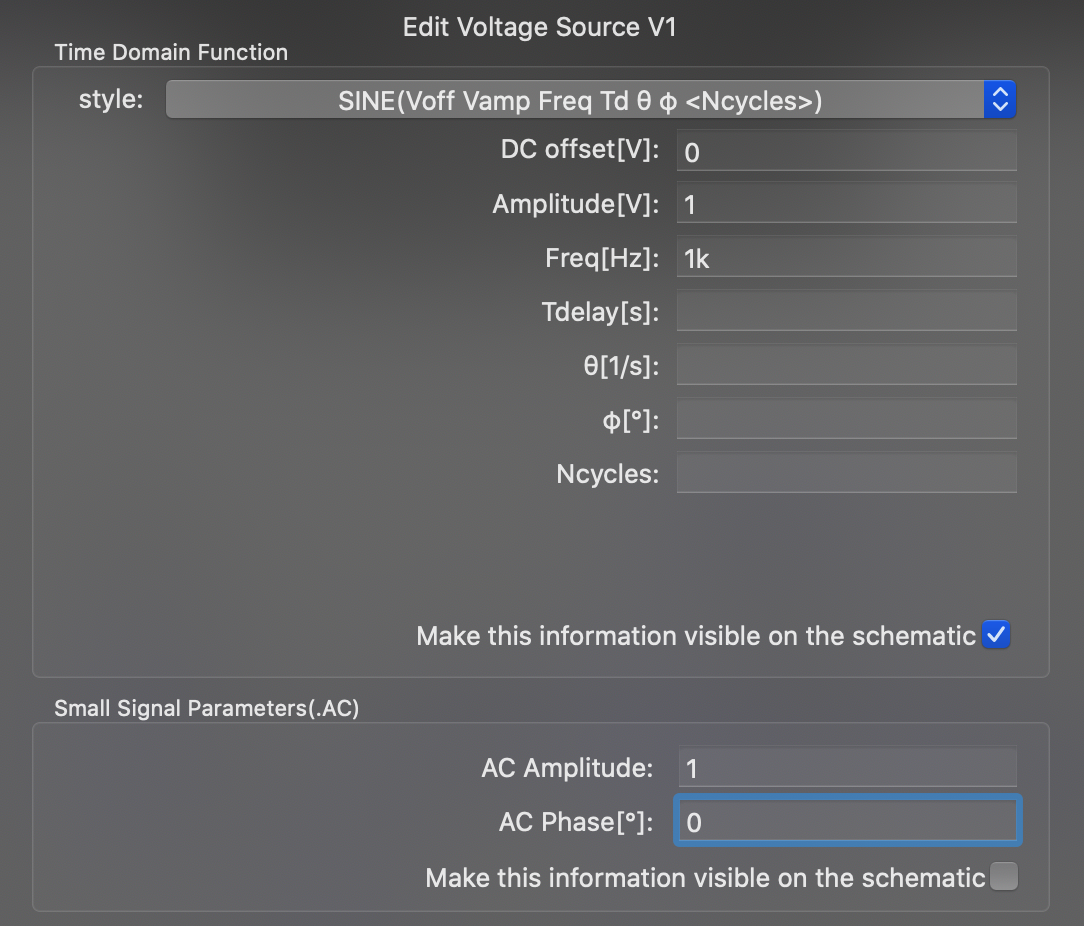
\includegraphics[width=0.8\linewidth]{pictures/ac_small_signal.png}
            \end{minipage} 
            & 
            \begin{minipage}{.5\textwidth}
            \begin{itemize}
              \item Wir verwenden die Schaltung aus dem vorherigen Beispiel!
              \item Wichtig ist hierbei, dass wir Spannungsquelle für den AC-Sweep konfigurieren
              Hierzu geht ihr per rechtem Mausklick in das advanced menu von V1 und stellt das Kleinsignal Verhalten (AC)
              auf \textbf{Amplitude 1V und Frequenz 1kHz}.
            \end{itemize}
            \end{minipage} 
            \\
          \end{tabular}
          \begin{tabular}{p{6cm} p{4cm}}
            \hline
            \textbf{Simulation und Analyse} & \\
            \hline \\
            \begin{minipage}{.6\textwidth}
              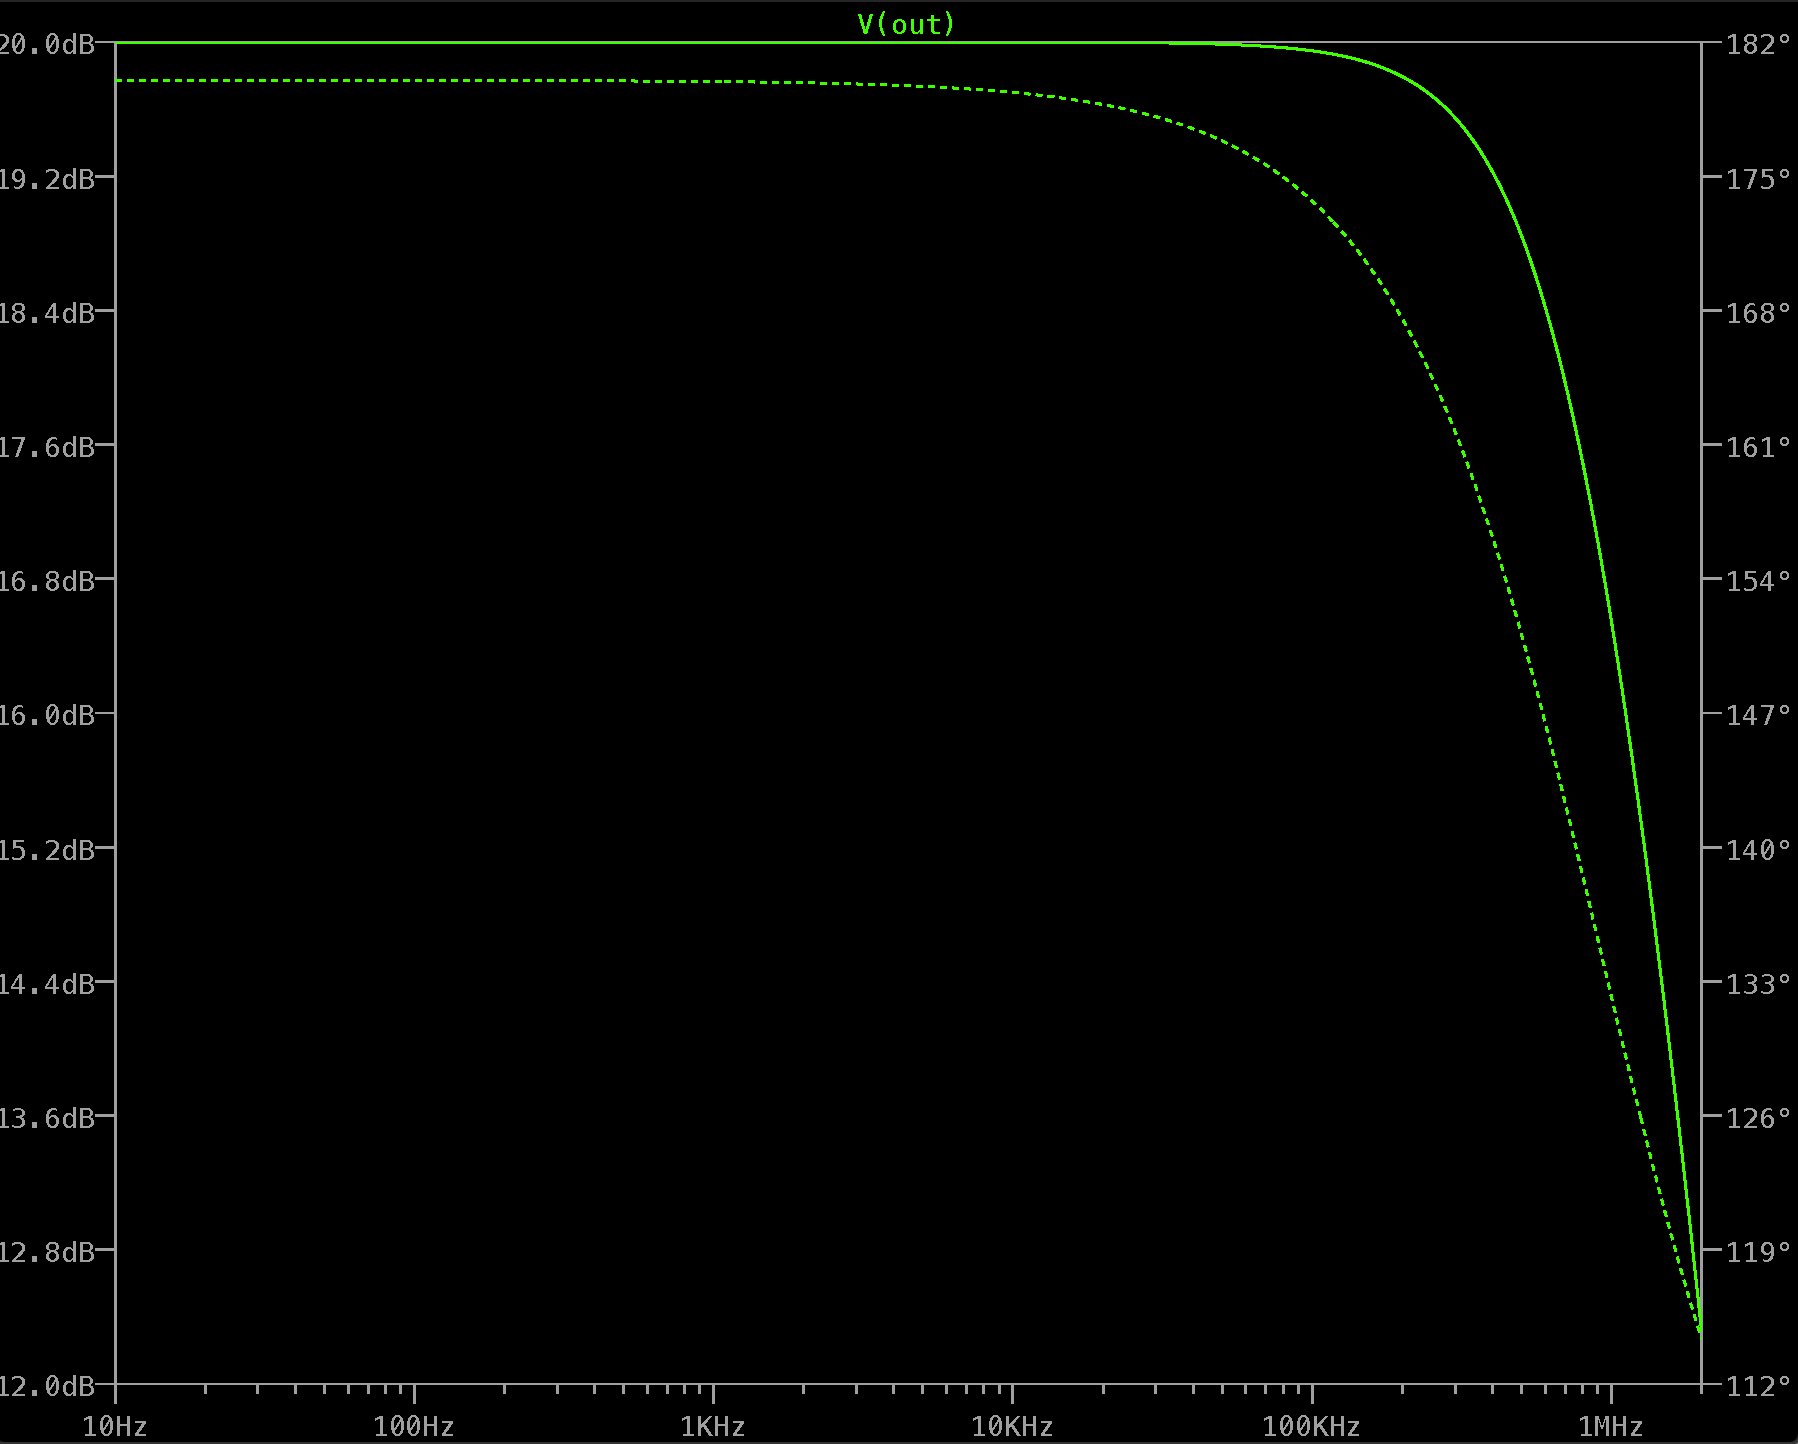
\includegraphics[width=0.7\linewidth]{pictures/analysis_6.png}
            \end{minipage} 
            & 
            \begin{minipage}{.4\textwidth}
            \begin{itemize}
              \item Klickt auf 
\includegraphics[scale=0.3]{pictures/run.png} (run) und LTspice startet die Simulation
              \item Fügt nun die Ausgangsspannung der Schaltung als Messpunkt hinzu.
              \item Im waveform viewer solltet ihr das Bode-Diagram mit Amplitude und Phase sehen.
            \end{itemize}
            \end{minipage} 
            \\
          \end{tabular}

        \end{table}
        
        \end{tiny} \end{spacing}

                    
      %\begin{spacing}{0.9} \begin{tiny}
      %  \begin{table}[h!]
      %    \begin{tabular}{p{10cm} }
      %      \hline
      %      \textbf{Ergebnis und Auswertung} \\
      %      \hline \\    
      %      Es muss das selbe Ergebnis herauskommen wie im vorherigen Experiment unter Verwendung des idealen OPV's \textbf{opamp}.
      %    \end{tabular}
      %  \end{table}
      %\end{tiny} \end{spacing}
        
         \end{frame}

         \begin{frame}[t]{OPV Schaltungen - Analyse der Grenzfrequenz einer Schaltung }
    
          \begin{spacing}{0.9} \begin{tiny}
            \begin{table}[h!]
            \begin{tabular}{p{10cm}}
              \hline
              \textbf{Simulation und Analyse} \\
              \hline \\
              \begin{minipage}{\textwidth}
                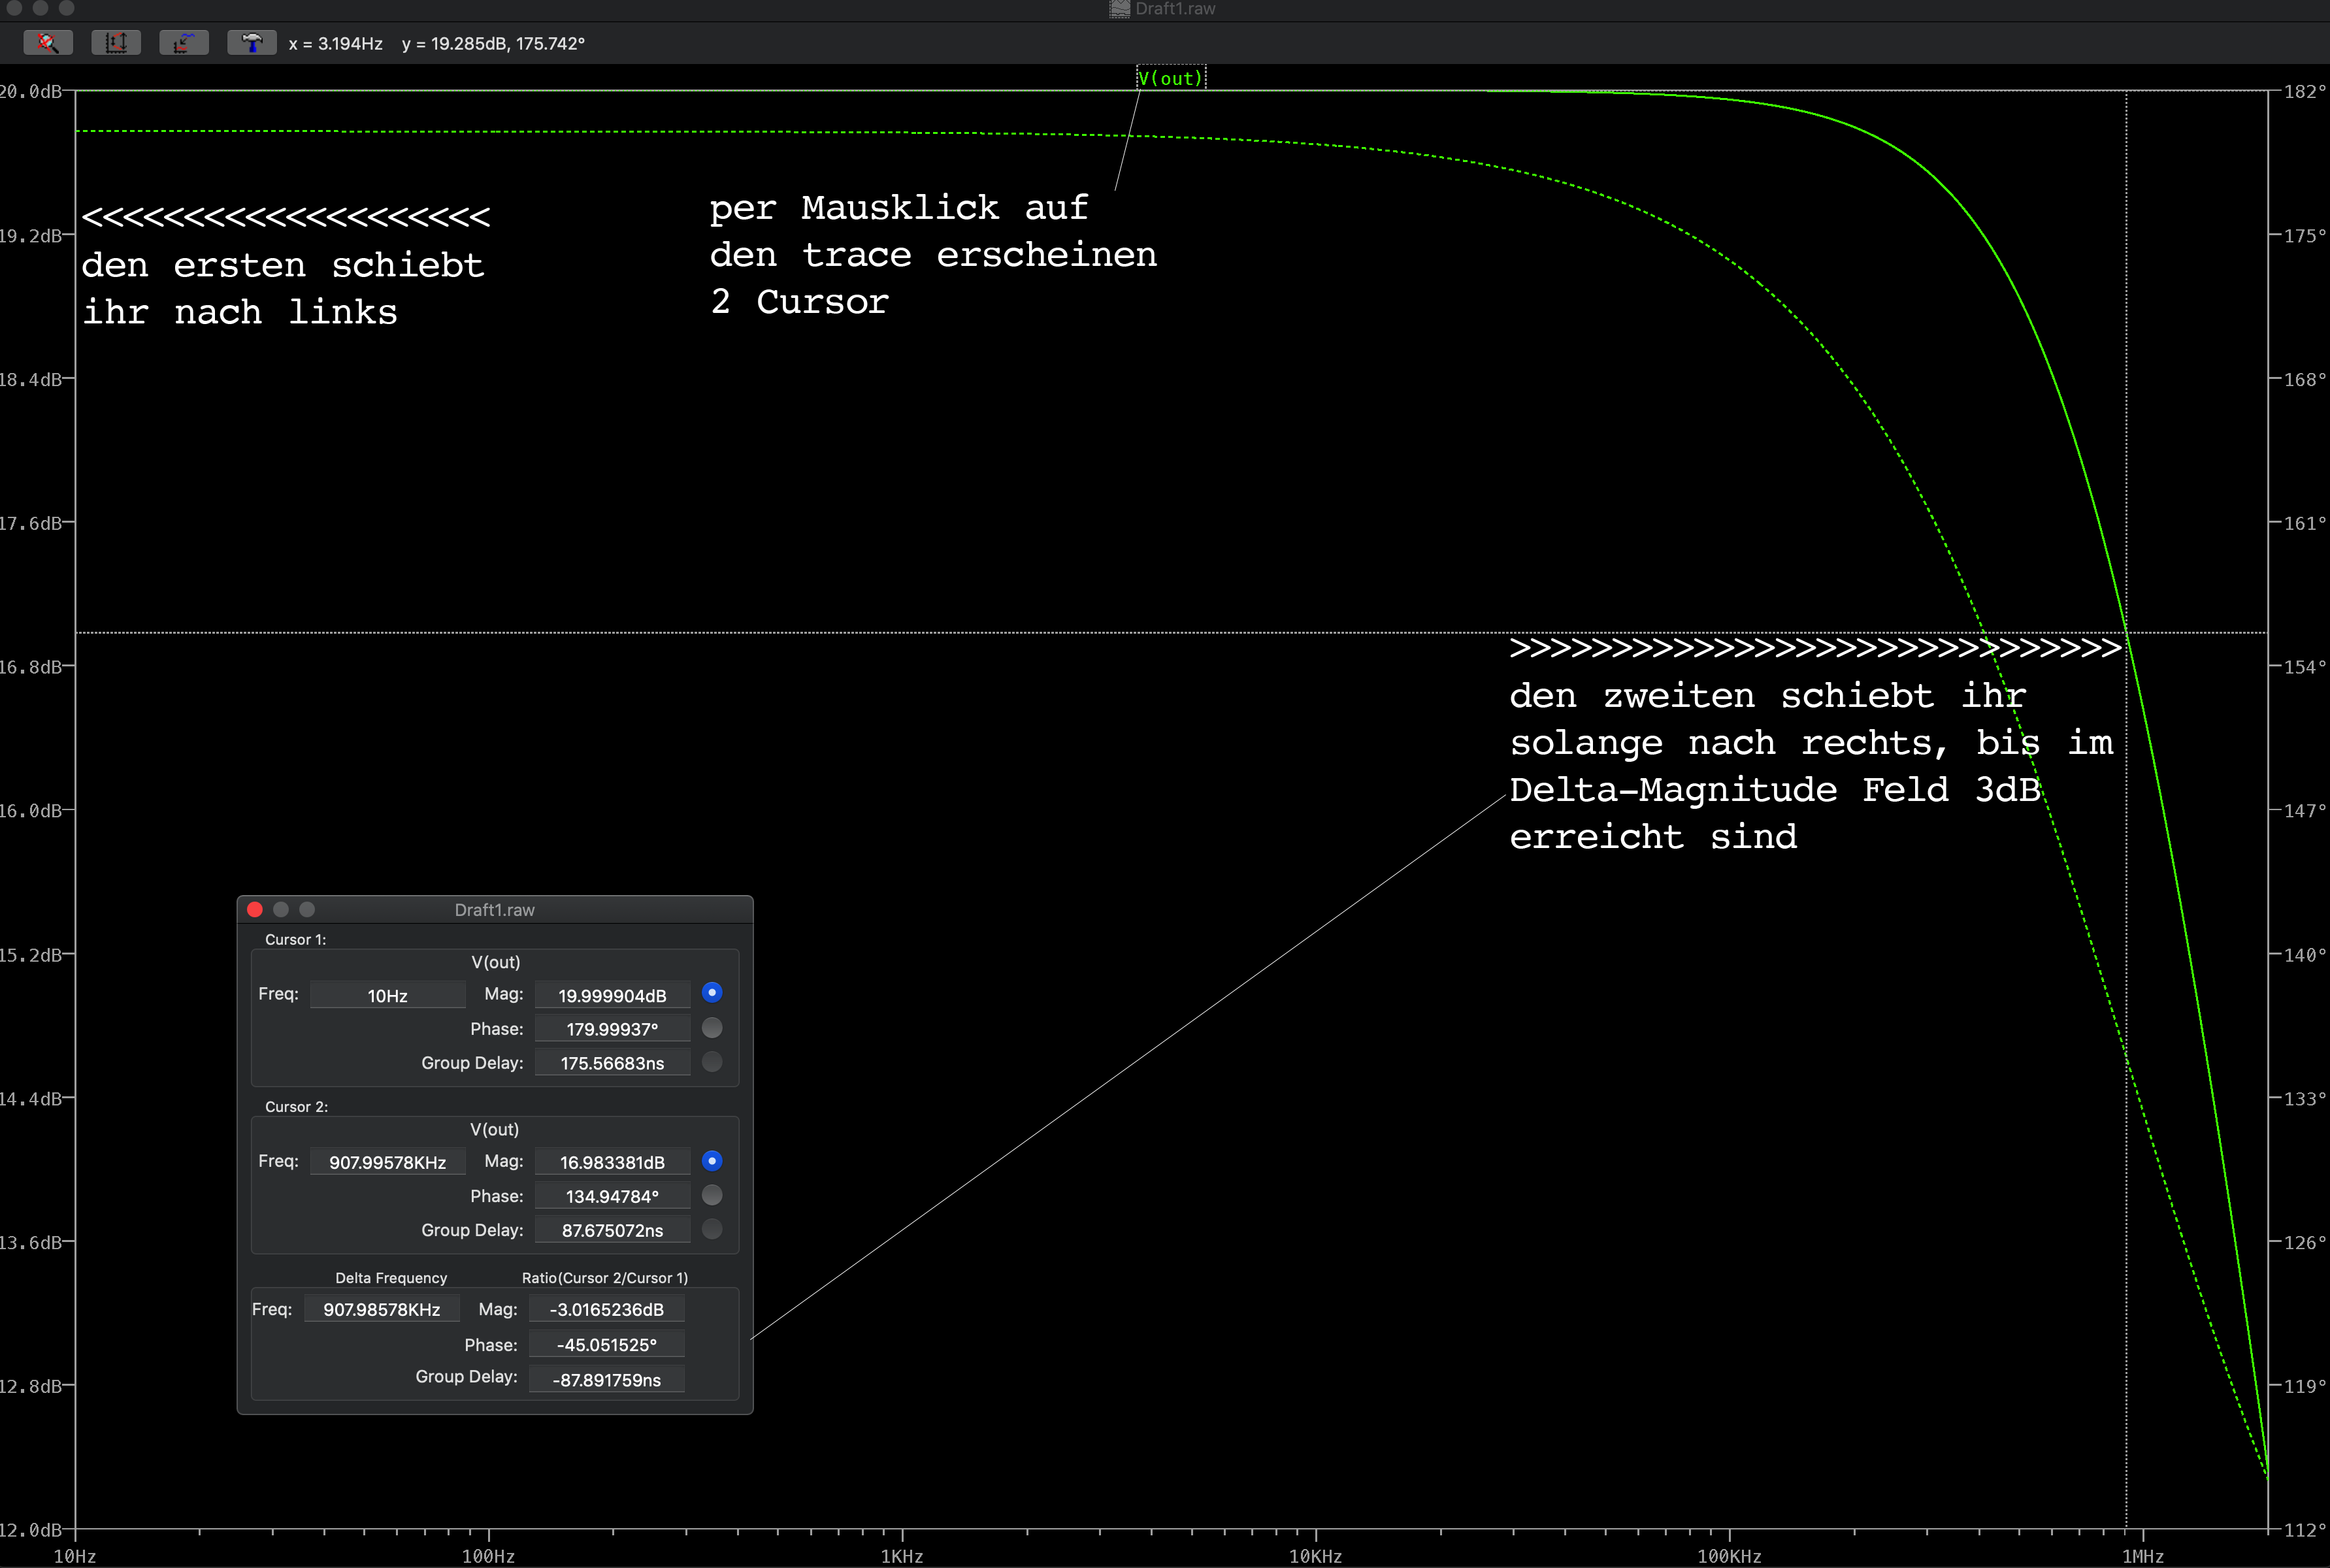
\includegraphics[width=\linewidth]{pictures/bode_1_remastered.png}
              \end{minipage} 
              \\
            \end{tabular}
  
          \end{table}
           
          \end{tiny} \end{spacing}
   
                      
        %\begin{spacing}{0.9} \begin{tiny}
        %  \begin{table}[h!]
        %    \begin{tabular}{p{10cm} }
        %      \hline
        %      \textbf{Ergebnis und Auswertung} \\
        %      \hline \\    
        %      Es muss das selbe Ergebnis herauskommen wie im vorherigen Experiment unter Verwendung des idealen OPV's \textbf{opamp}.
        %    \end{tabular}
        %  \end{table}
        %\end{tiny} \end{spacing}
          
           \end{frame}


         \begin{frame}[t]{OPV Schaltungen - nicht-invertierender Verstärker}

          \textbf{Ziel - Anwendung der Kenntnisse}
    
          \begin{spacing}{0.6} \begin{tiny}
          
          Nachfolgend könnt ihr die Schaltung für einen nicht-invertierenden Verstärker in einer OPV Schaltung sehen. 

          \begin{enumerate}
            \item Baut die Schaltung auf, dimensioniert sie so, dass Sie einen Verstärkungsfaktor
            \item Verwendet die UniversalOpamp2 aus der vorherigen Übrung mit einer Versorgungsspannung von +/-12V
            \item Verifiziert eure Schaltung und das \textbf{nicht-invertierende} Verhalten mit einer transienten Simulation von 0 - 50ms.
            \item Wählt dabei eine ausreichend kleine Schrittweite
            \item Wechselt die Simulationsart zum AC-Sweep und ermittelt die Grenzfrequenz
          \end{enumerate}

            \begin{table}[h!]
              \begin{tabular}{p{5cm} p{5cm}}
                \begin{minipage}{.5\textwidth}
                  \begin{figure}
                    \scalebox{0.35}{
                  \centering
                  \begin{circuitikz}
                    \ctikzset{bipoles/length=1cm}
                    \draw
                    (0,0) node[op amp,yscale=-1](opamp){} 
                    (opamp.+) to[short,-o] ++ (-2,0) to [V=$v_1$] ++ (0,-3) to ++(0,0) node[ground] {}
                    (opamp.-) to[short] ++ (0,-1.25) coordinate(X) to[R,l_=$R_1$] ++(0,-1) node[ground]{}
                    (opamp.out) to[R,l_=$R_2$] ++ (0,-1.5) coordinate(Y) to[short] ++ (-1.7,0) coordinate(X){}
                    (opamp.out) to[short,*-o] ++ (0.5,0) node[right]{$v_{\rm out}$}
                    ;
                    \end{circuitikz} 
                    }
                    
                \end{figure}
                \end{minipage} 
                & 
                \begin{minipage}{.5\textwidth}
                \begin{equation}
                  V_{out}=(1+\frac{R2}{R1})V_{1}
                  \end{equation}
                \end{minipage} 
              \end{tabular}
            
            \end{table}

            Spoiler! - Die Lösungen folgen auf den folgenden Folien. Wenn sie sich nicht sicher sind, schauen Sie einfach nach.\newline\newline
            Info! - Besonders die Analyse von Grenzfrequeznen ist für Ihre weitere Vorlesungzeit (Filter höhrerer Ordnung, EMV) hilfreich,
            da Sie neben der simulativen Bestätigung Ihrer Schaltungen auch theoretische Rechenaufgaben simulieren und so Ihre Rechnung
            verifizieren können.
            
            \end{tiny} \end{spacing}
           \end{frame}

          \begin{frame}[t]{OPV Schaltungen - Lösung transient}

              \begin{spacing}{0.9} \begin{tiny}
                \begin{table}[h!]
                \begin{tabular}{p{10cm}}
                  \hline
                  \textbf{Simulation und Analyse} \\
                  \hline \\
                  \begin{minipage}{\textwidth}
                    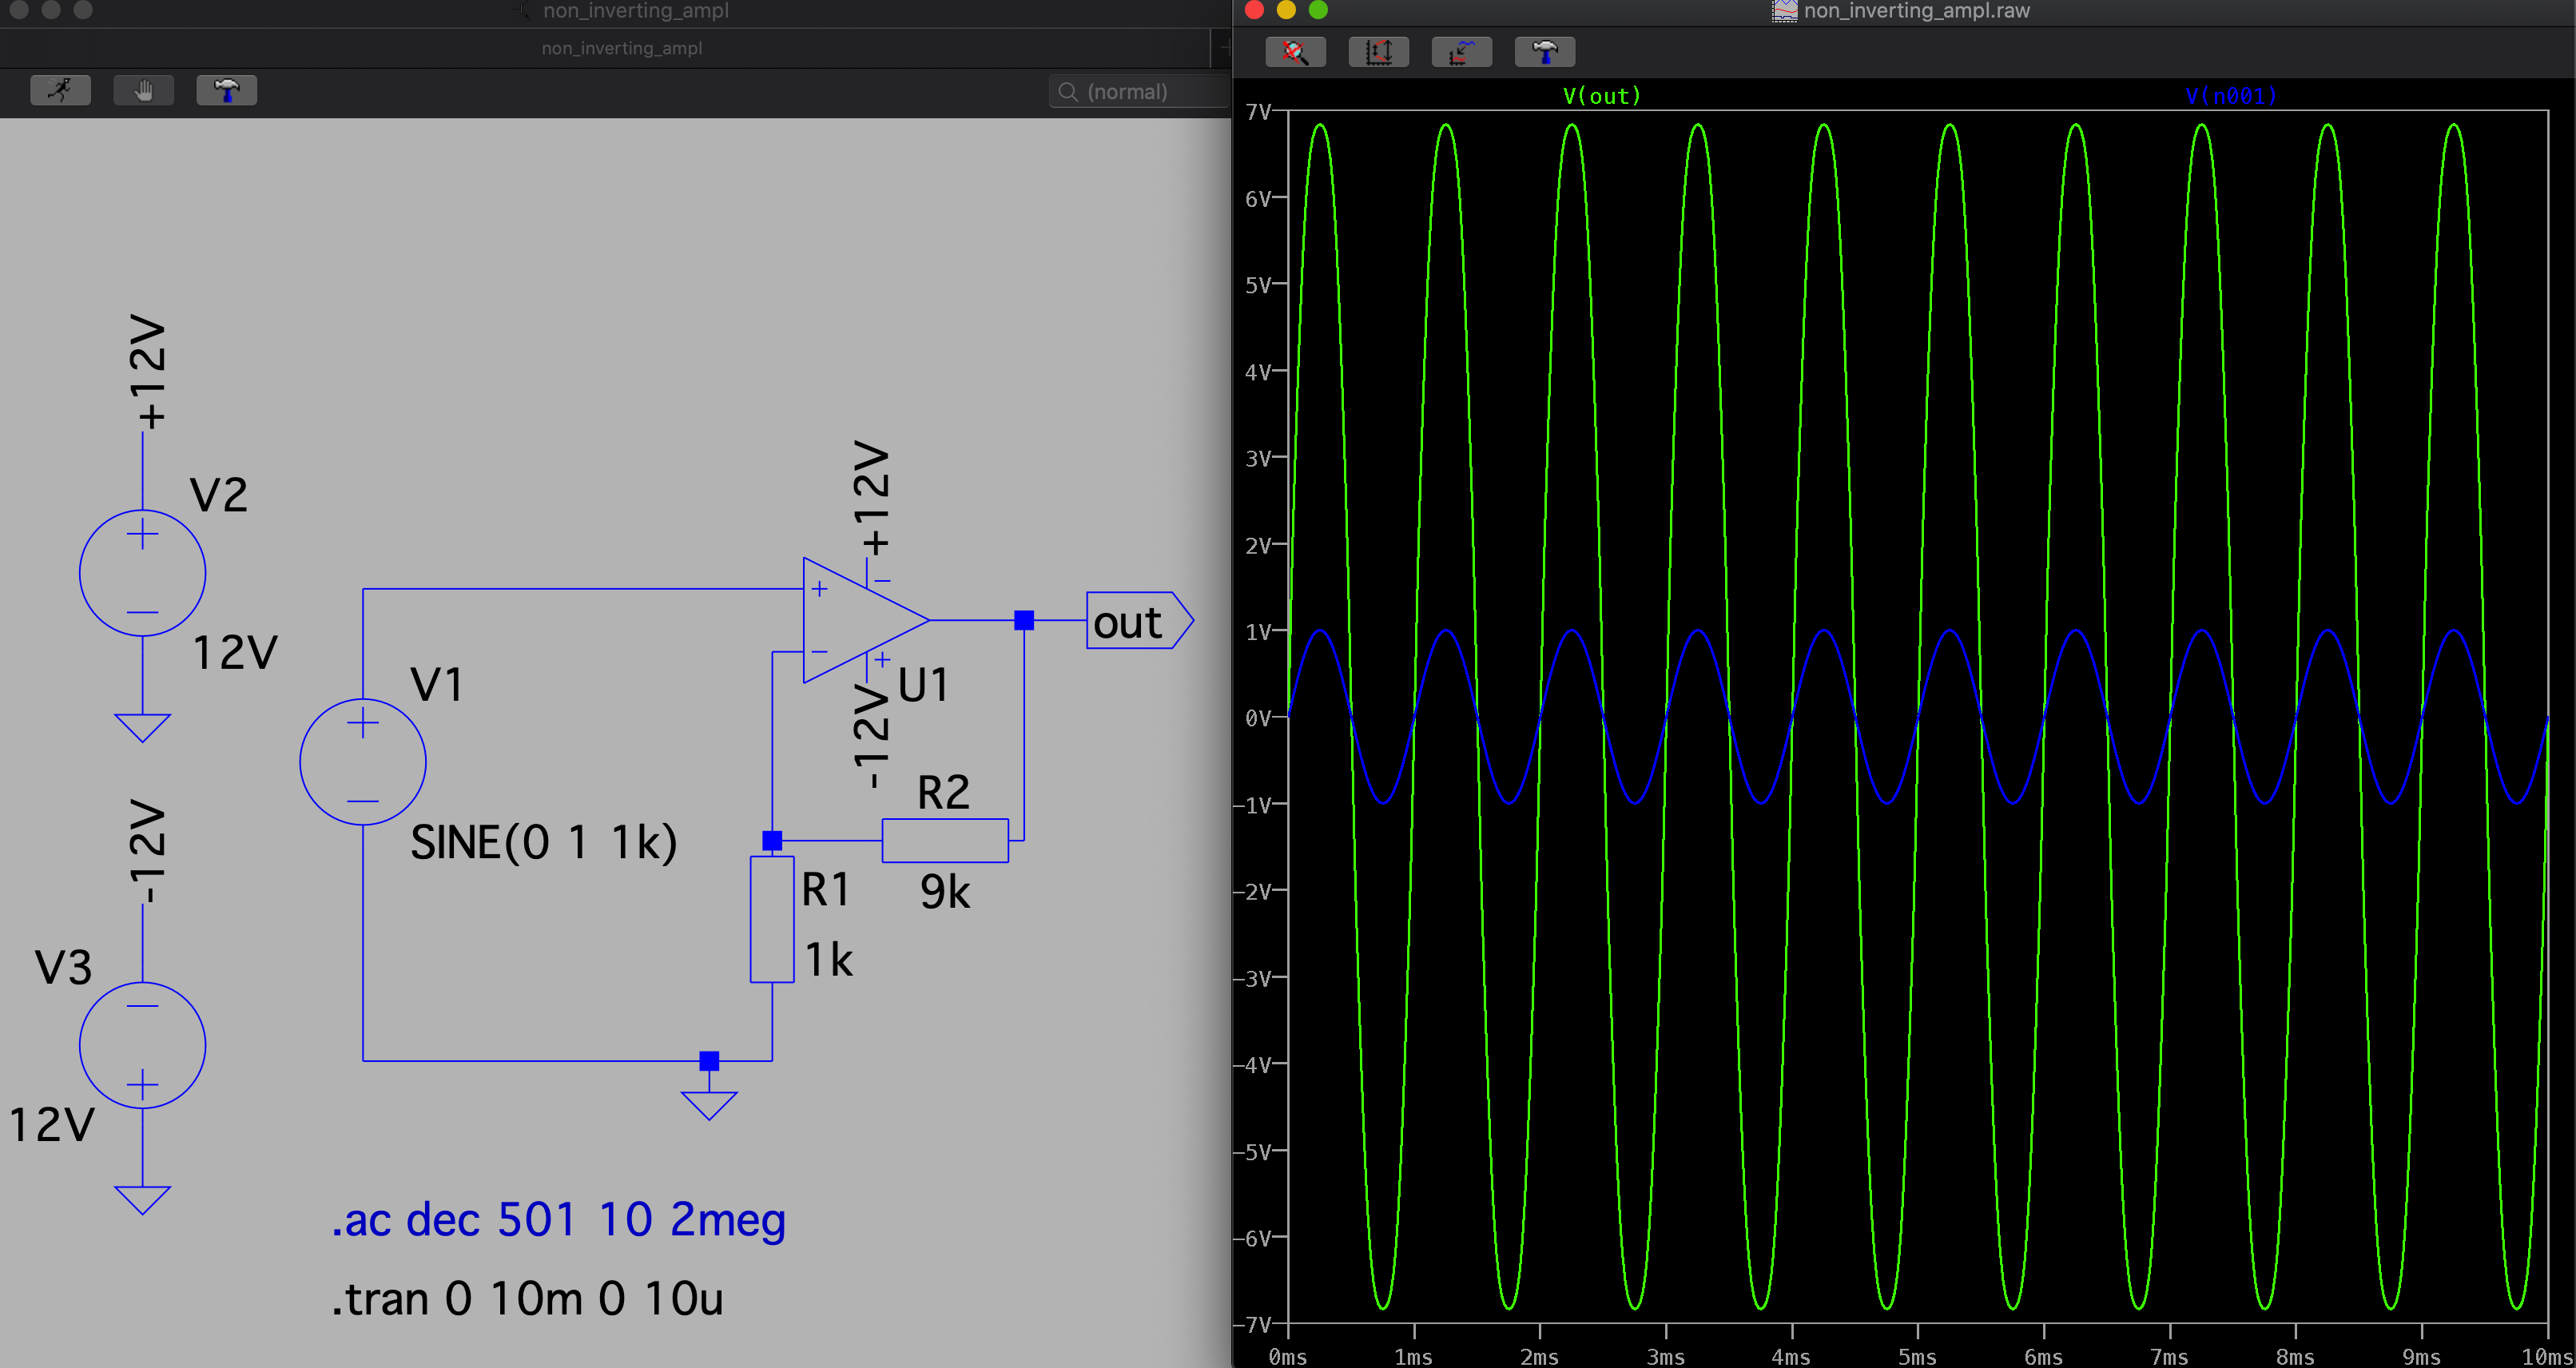
\includegraphics[width=\linewidth]{pictures/analysis_7.png}
                  \end{minipage} 
                  \\
                \end{tabular}
      
              \end{table}
               
              \end{tiny} \end{spacing}

          \end{frame}

          \begin{frame}[t]{OPV Schaltungen - Lösung Grenzfrequenz} 
    
              \begin{spacing}{0.9} \begin{tiny}
                \begin{table}[h!]
                \begin{tabular}{p{10cm}}
                  \hline
                  \textbf{Simulation und Analyse} \\
                  \hline \\
                  \begin{minipage}{\textwidth}
                    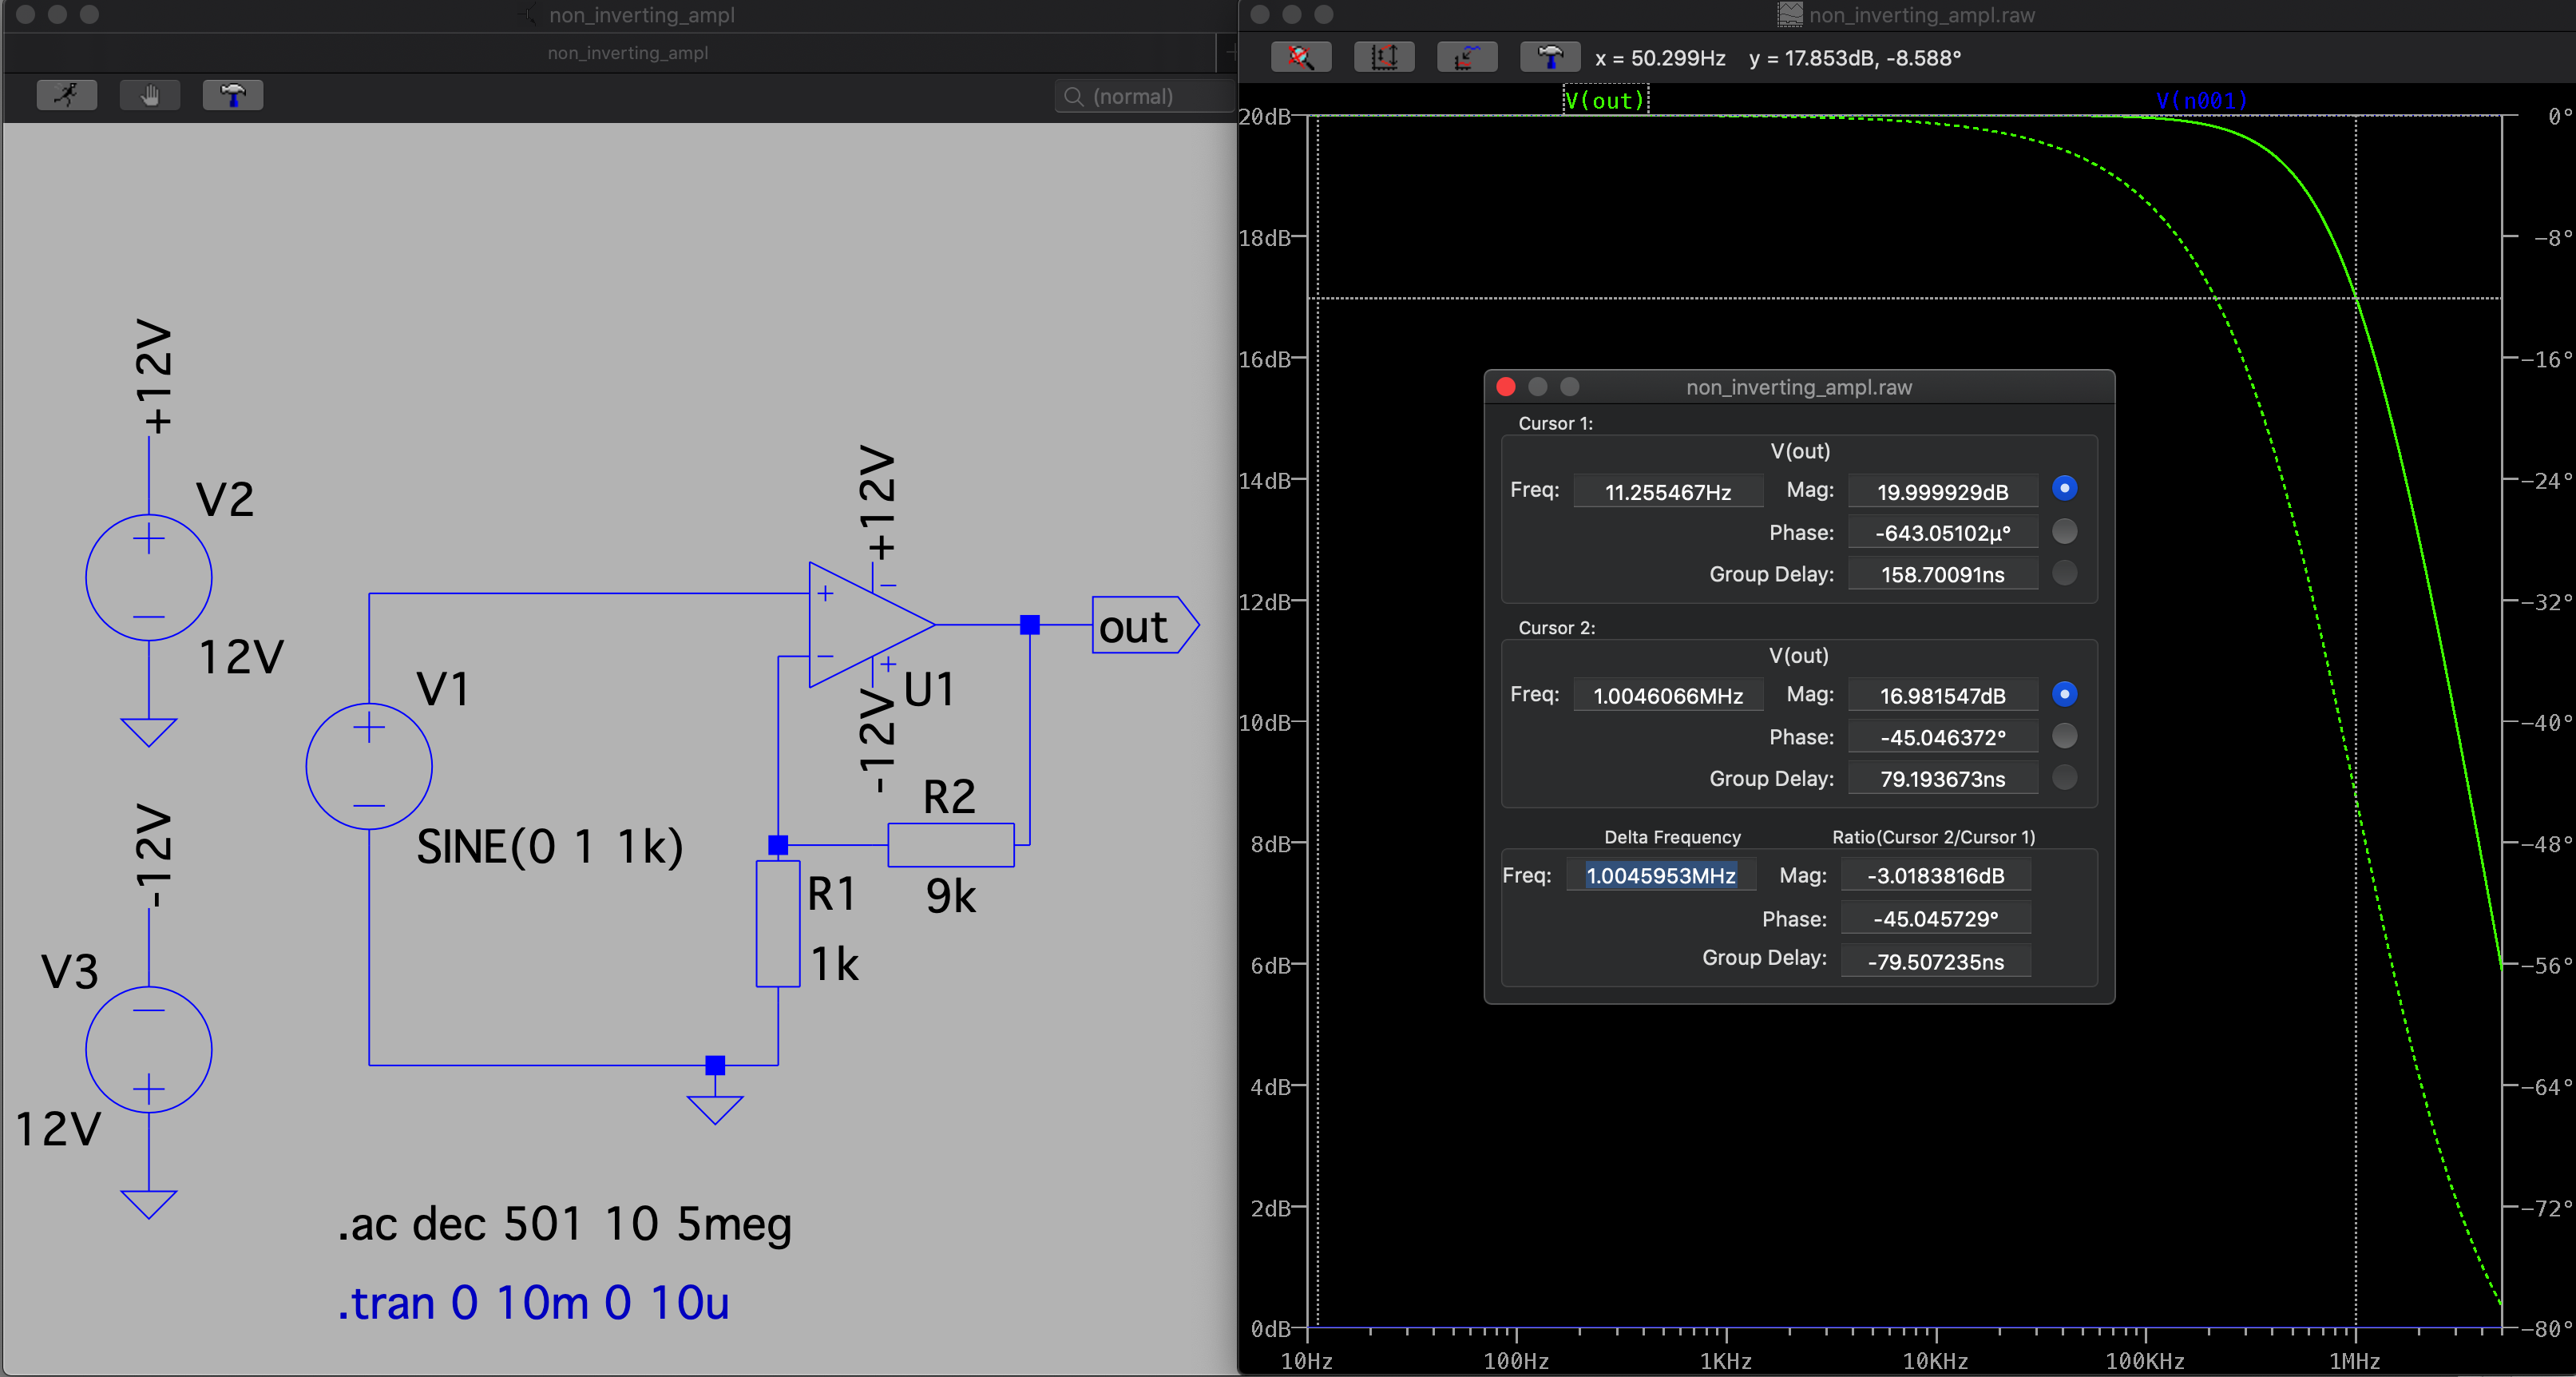
\includegraphics[width=\linewidth]{pictures/bode_2.png}
                  \end{minipage} 
                  \\
                \end{tabular}
      
              \end{table}
               
              \end{tiny} \end{spacing}

          \end{frame}%opv-transient, ac, non inverting

\section{Simulation vs. Realität}

\begin{frame}[t]{Wheatstone Bridge}

  Die Wheatstone Bridge ist eine einfache Schaltung um einen Wiederstand zu messen. Die Schaltung gilt als abgeglichen, wenn an $V_{AB}$ keine Spannng anliegt.

  Die theoretische Herleitung ist nicht ganz trivial, daher möchten wir an dieser Stelle die Realität und den Aufwand eines praktischen Aufbaus der Flexibilität einer Simulation gegenüberstellen.


  \begin{figure}
    \scalebox{0.6}{
      \centering
      \begin{circuitikz}
        \ctikzset{bipoles/thickness=1}
        \ctikzset{bipoles/length=.6cm}
        \draw
        (0,0) to [short, *-] (4,0)
        (0,0) to [V, l_=$V_{1}$] (0,-4)
        (2,0) to (2,-0.5)
        (4,0) to (4,-0.5)
        (2,-0.5) to [R, l_=$R_{1}$] (2,-1.5)
        (2,-2.5) to [R, l_=$R_{2}$] (2,-3.5)
        (2,-1.5) to (2,-2.5)
        (2,-2) to [short,*-o] (2.25,-2) node[right]{$V_{a}$}
        (4,-1.5) to (4,-2.5)
        (4,-2) to [short,*-o] (4.25,-2) node[right]{$V_{b}$}
        (4,-0.5) to [R, l_=$R_{3}$] (4,-1.5)
        (4,-2.5) to [R, l_=$R_{4}$] (4,-3.5)
        (2,-3.5) to (2,-4)
        (4,-3.5) to (4,-4)
        (0,-4) node[ground]{}
        (2,-4) node[ground]{}
        (4,-4) node[ground]{}
        ;
      \end{circuitikz}
    }
  \end{figure}

\end{frame}

\begin{frame}[t]{Experiment}

  Wir werden jetzt den folgenden Aufbau "live" analysieren. Beachtet, dass die Schaltung komplexer ist als in dem einleitenden schematischen Aufbau - wie immer.

  \begin{spacing}{0.9} \begin{tiny}
      \begin{minipage}{\textwidth}
        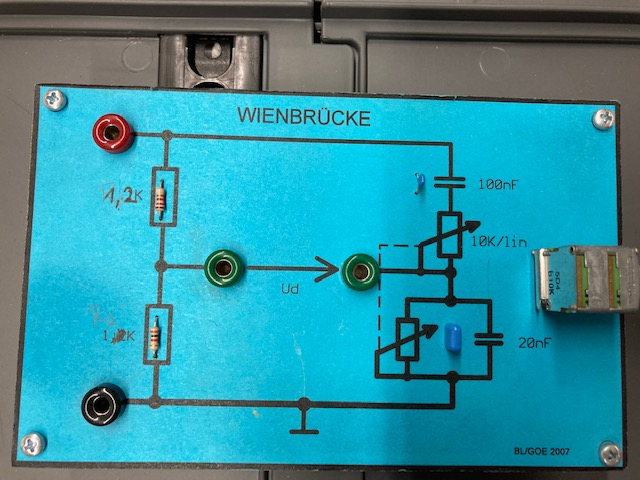
\includegraphics[width=0.5\linewidth]{pictures/wheatstone_bridge.jpg}
      \end{minipage}
    \end{tiny} \end{spacing}

  \textbf{Leitet aus der gemessenen Spannung den Wiederstandswert her.}

\end{frame}


\begin{frame}[t]{Simulation - Vorgehen}

  Wir wollen die Wienbrücke bei einer festen Spannungsversorgung $Sine(0\ 1\ 5k)$ abgleichen.
  \begin{itemize}
    \item Hierfür variieren wir den Trimmer bis die Differenzspannung $U_{AB}$ null beträgt.
    \item Via LTspice können wir uns dem abgeglichen Zustand annähern, indem wir den Trimmer als Variable betrachten.
    \item Hierfür nutzen wir die Variable $RT$ mit der Spice directive $.step\ param\ RT\ Anfangswert\ Endwert\ Inkrement$ und tasten uns an die ideale Trimmereinstellung heran.
    \item Mittels der Funktion select steps ermitteln wir die am besten abgeglichen Widerstände und passen unsere Variable sukzessive an.
  \end{itemize}

\end{frame}

\begin{frame}[t]{Simulation - Transient}

  Bitte baut die unten stehende Schaltung nach und führt das Experiment durch.

  \begin{spacing}{0.9} \begin{tiny}
      \begin{minipage}{\textwidth}
        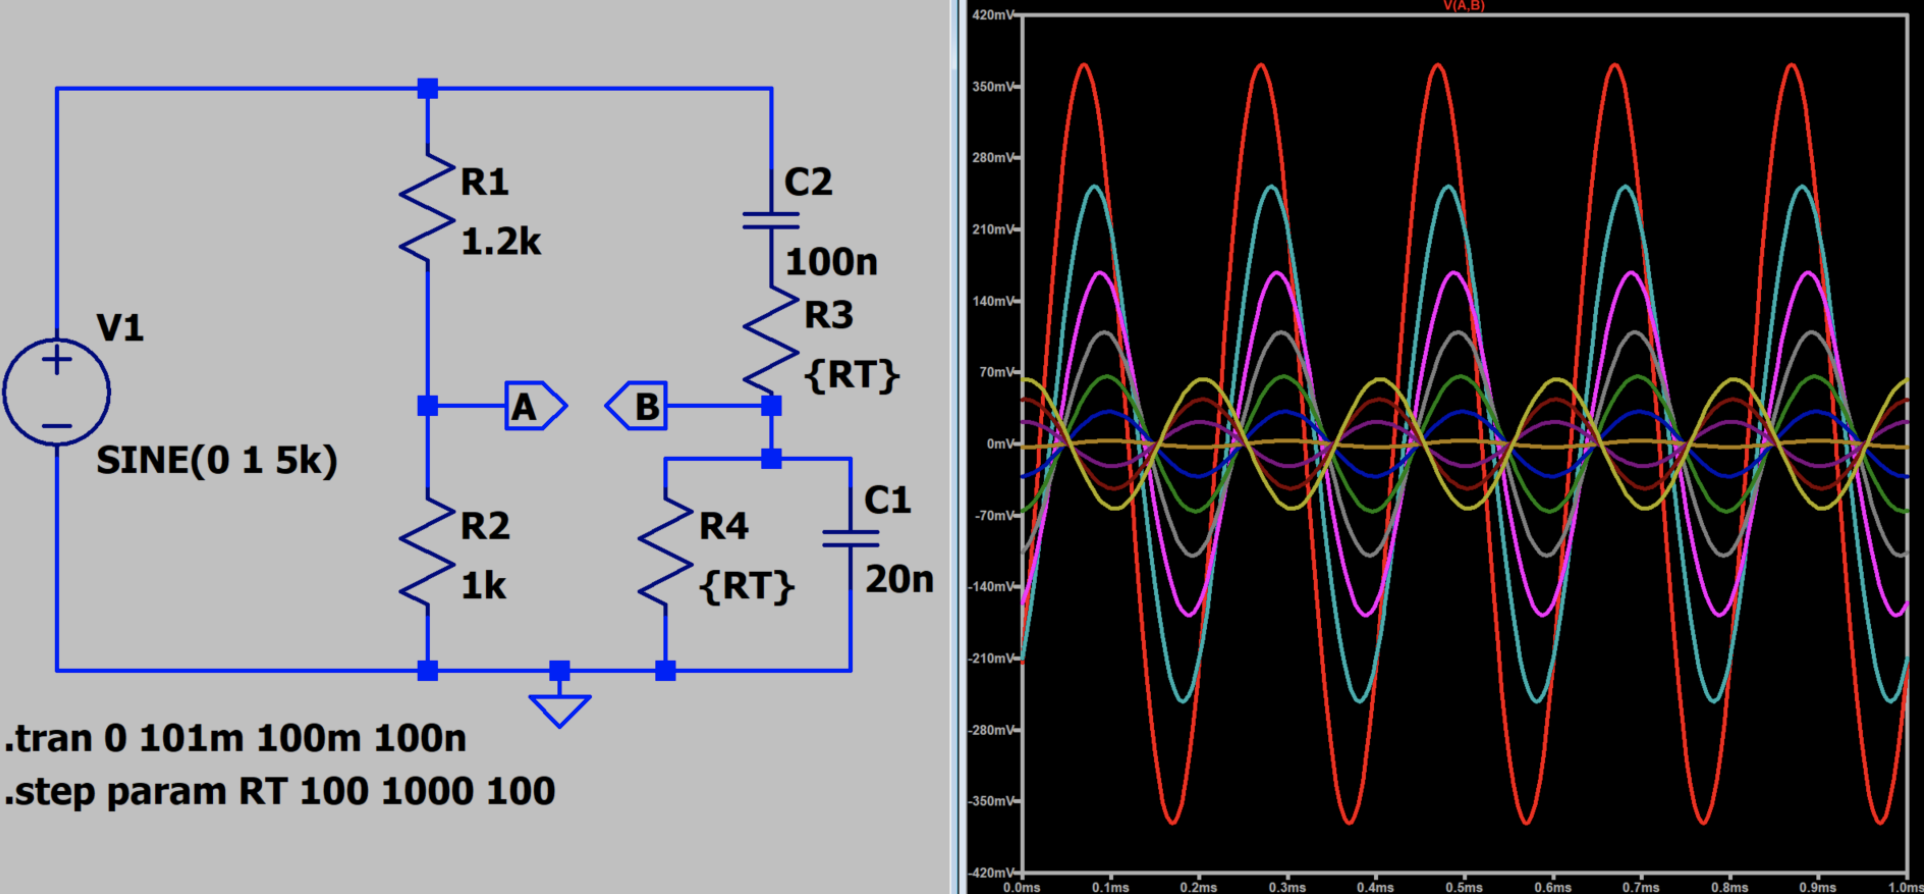
\includegraphics[width=0.75\linewidth]{pictures/wheatstone_simulation.png}
      \end{minipage}
    \end{tiny} \end{spacing}

  \textbf{Bei etwa $712\Omega$ ist die Brücke abgeglichen - wir ersetzen die Variable durch einen festen Widerstandswert.}

\end{frame}

\begin{frame}[t]{Simulation - AC}

  Simulieren wir nun das Verhalten über die Frequenz via AC Analysis.

  \begin{spacing}{0.9} \begin{tiny}
      \begin{minipage}{\textwidth}
        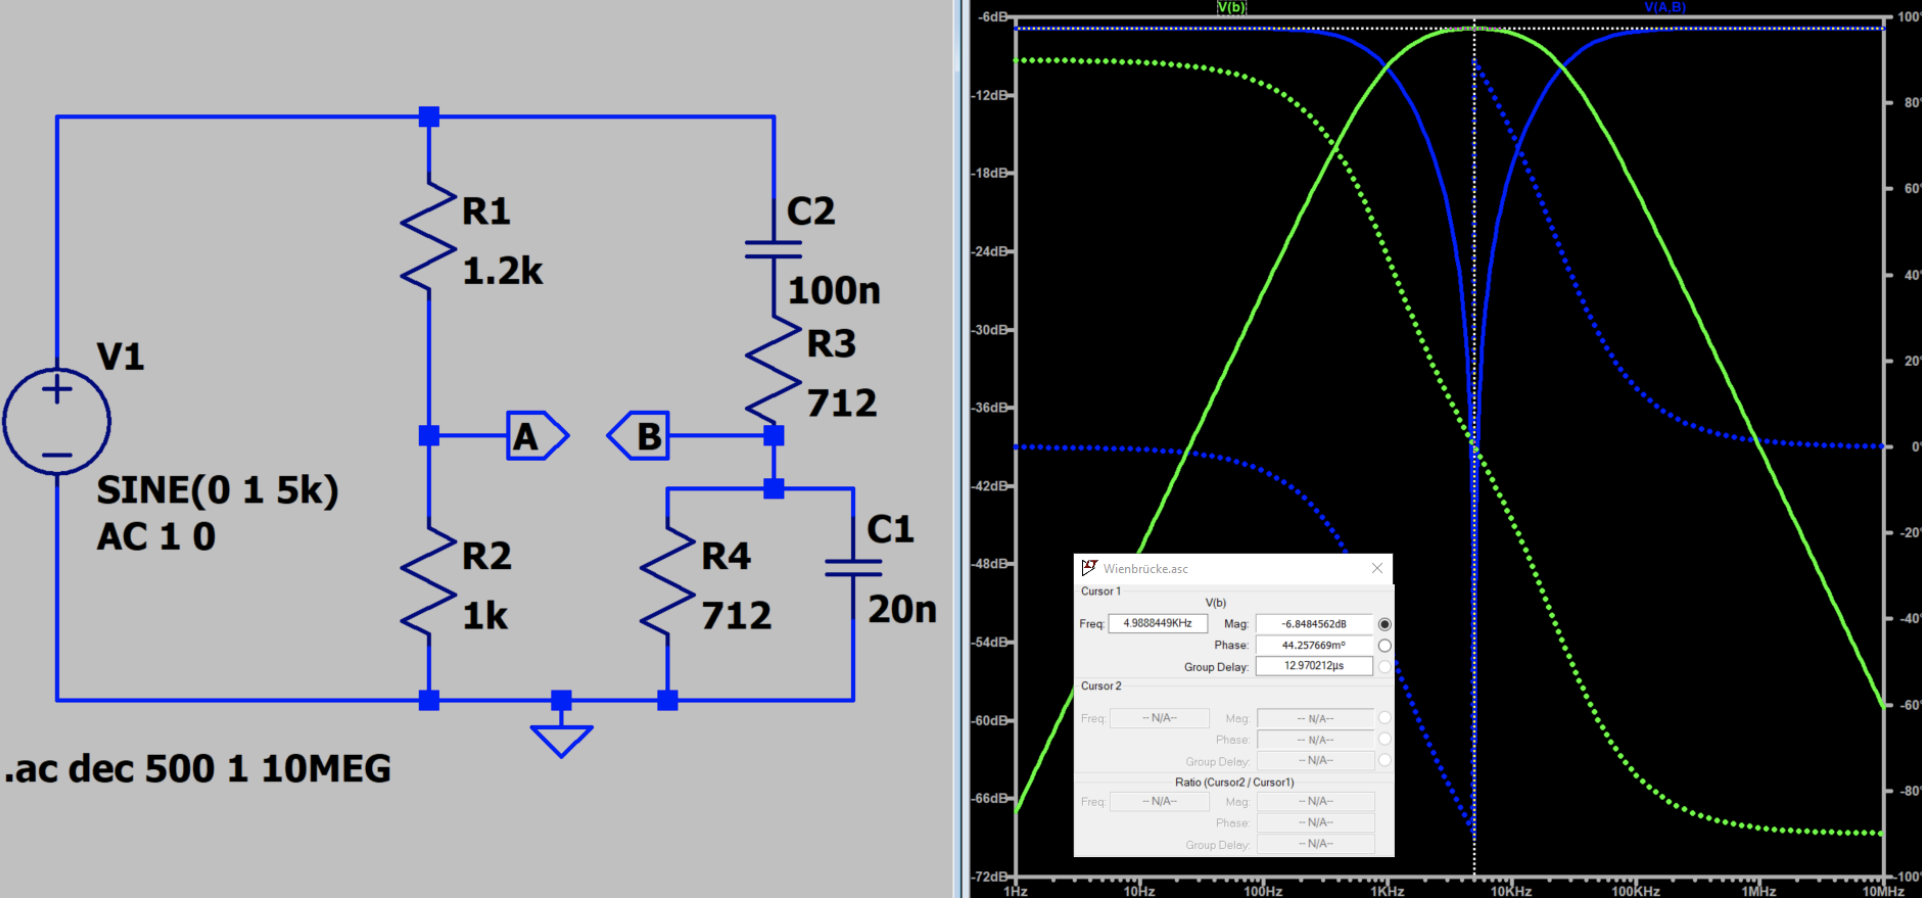
\includegraphics[width=0.75\linewidth]{pictures/wheatstone_ac.png}
      \end{minipage}
    \end{tiny} \end{spacing}

\end{frame}

\begin{frame}[t]{Simulation - AC Analyse}

  Betrachten wir zunächst die Spannung $U_A$, bzw. $U_B$.

  \begin{itemize}
    \item Im rechten Teilzweig der Schaltung ergibt sich durch den in Reihe verbauten Tiefpass und Hochpass ein Bandpassverhalten.
    \item Lediglich in einem mittleren Frequenzbereich um 5kHz ergibt sich eine Spannung $U_{AB}$.
  \end{itemize}

  Hieraus resultiert ein umgekehrtes Verhalten der Differenzspannung $U_{AB}$. Hier zeigt sich das Verhalten einer Bandsperre.
  Die Differenzspannung $U_{AB}$ ist bei 5kHz ideal abgeglichen und die Spannungen $U_{A}$ und $U_{B}$ heben sich gegenseitig auf.
\end{frame}

\begin{frame}[t]{Simulation - AC Grenzfrequenzen}

  Die Schaltung hat ja nach Betrachtung ein Bandpass- bzw. Bandsperrverhalten. Wir bestimmen die Grenzfrequenzen für beiden Messpunkte, $U_A$ und $U_{AB}$.
  \begin{itemize}
    \item $U_A$ Bandpass - \textbf{977 kHz}
    \item $U_{AB}$ Bandsperre - \textbf{977 kHz}
  \end{itemize}

  \begin{figure}
    \centering
    \subfloat{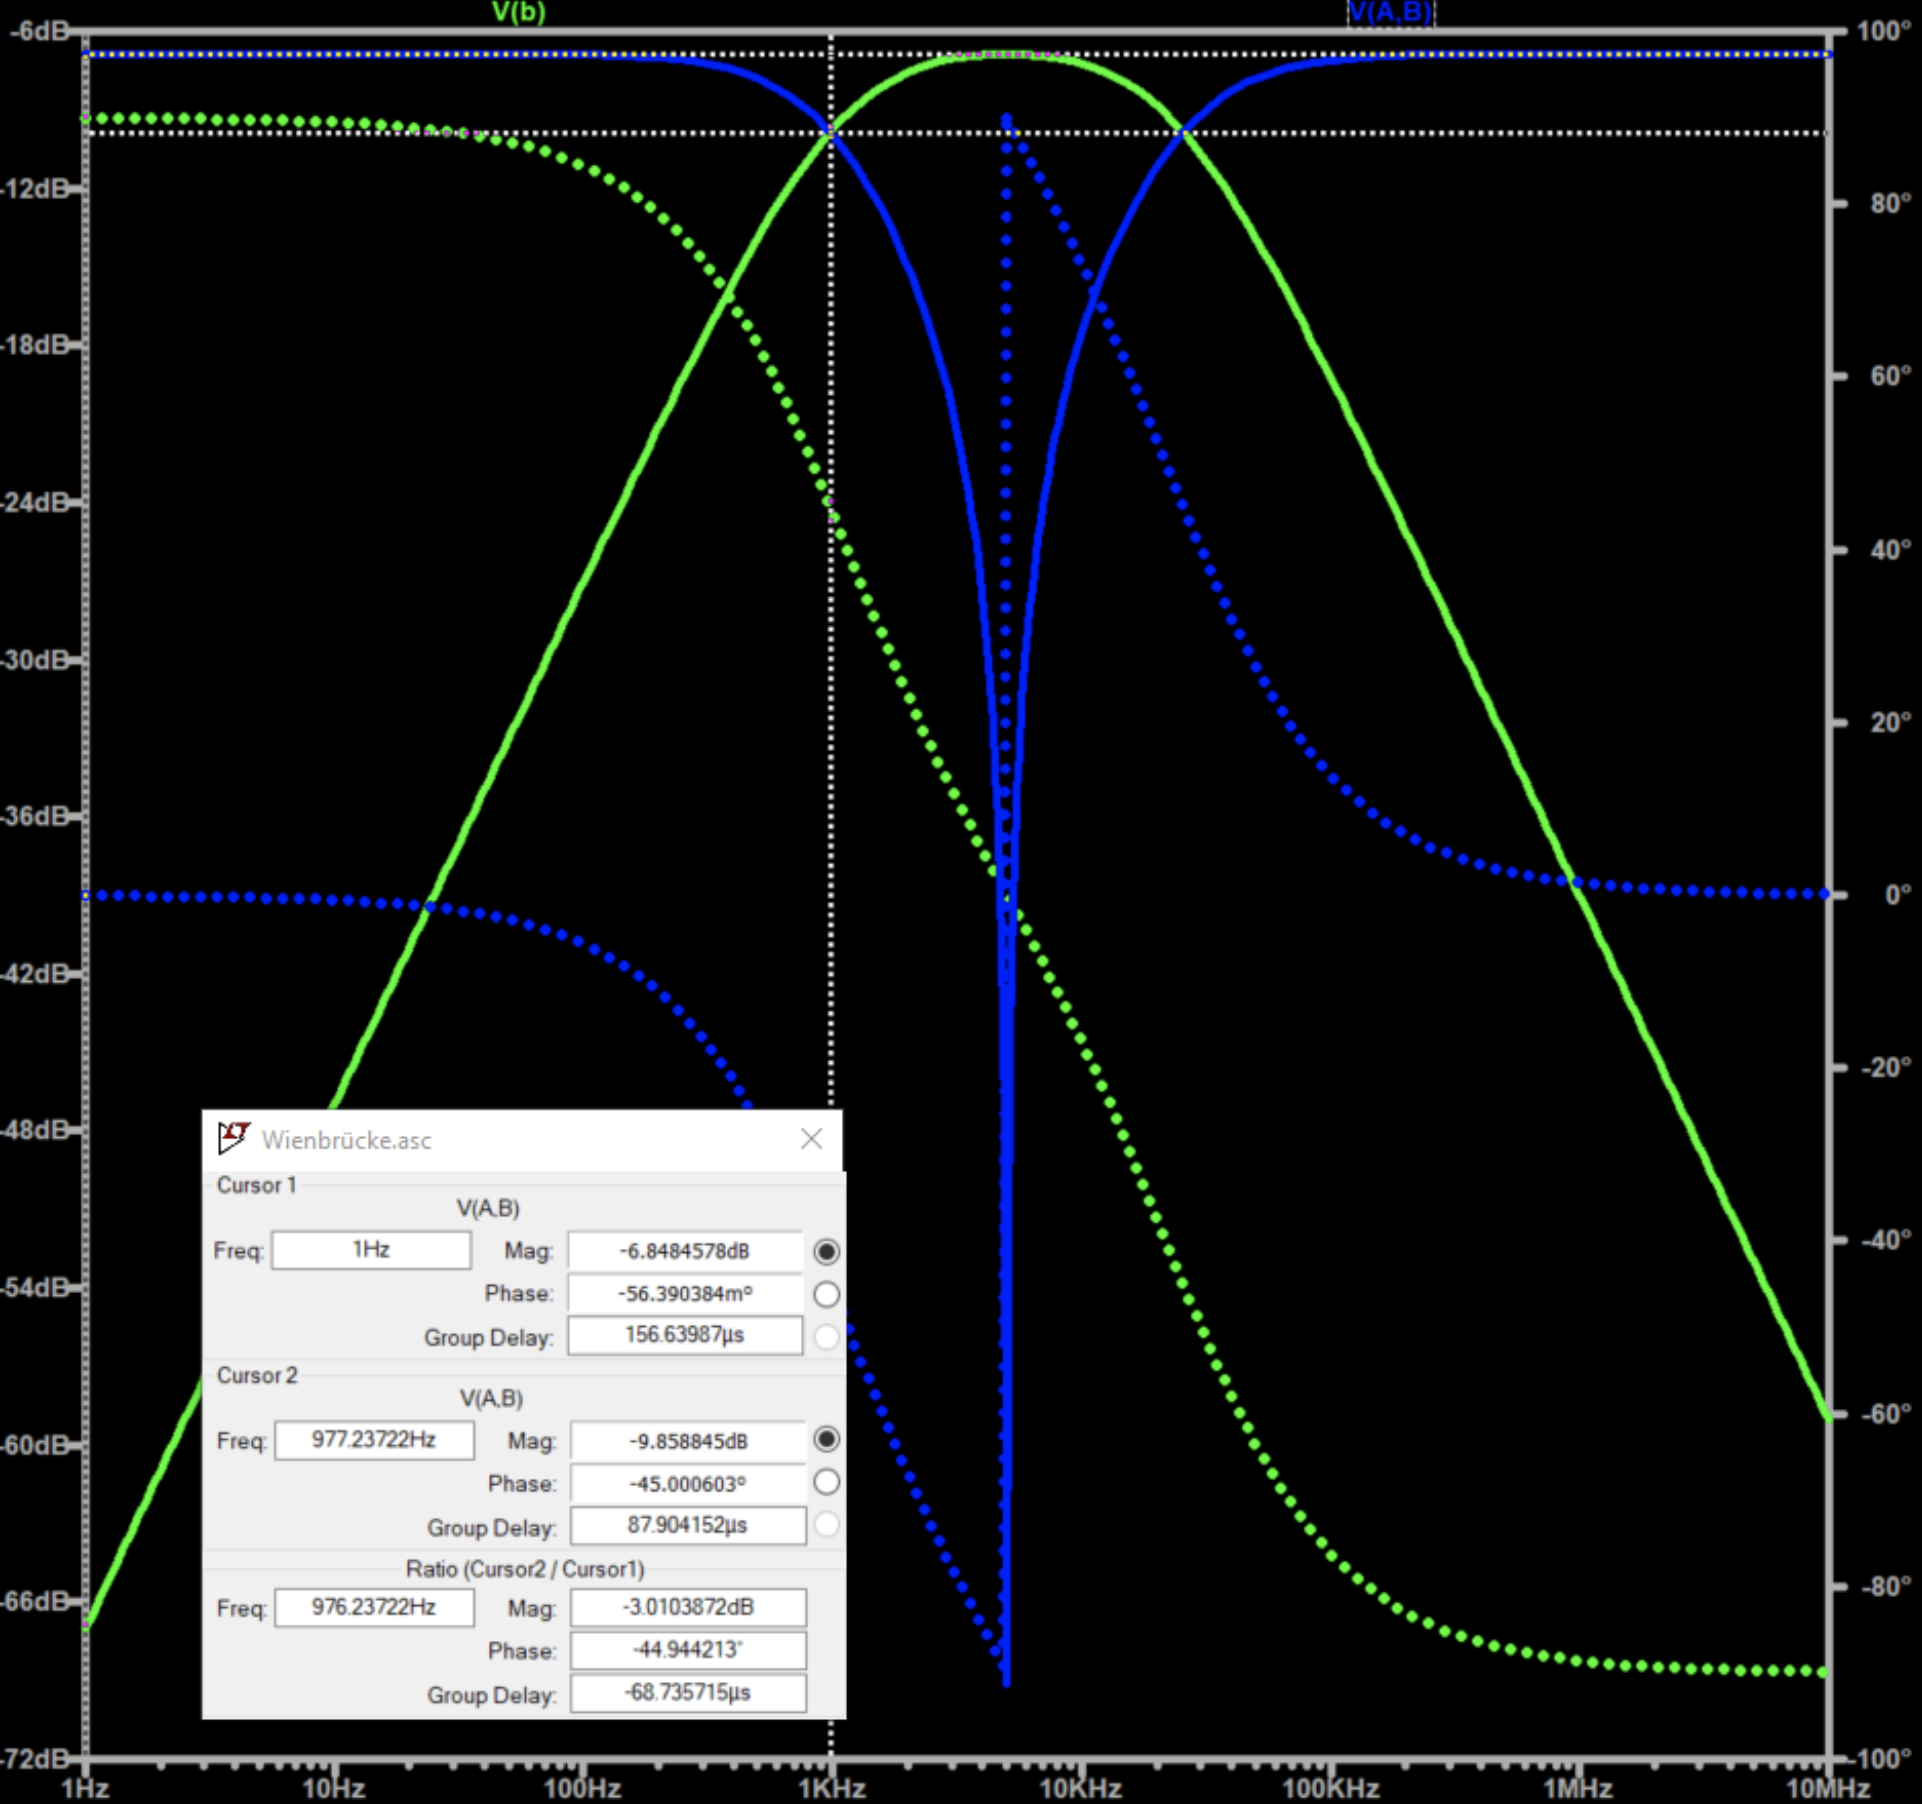
\includegraphics[width=4.5cm]{pictures/Bandpass.png}}\qquad
    \subfloat{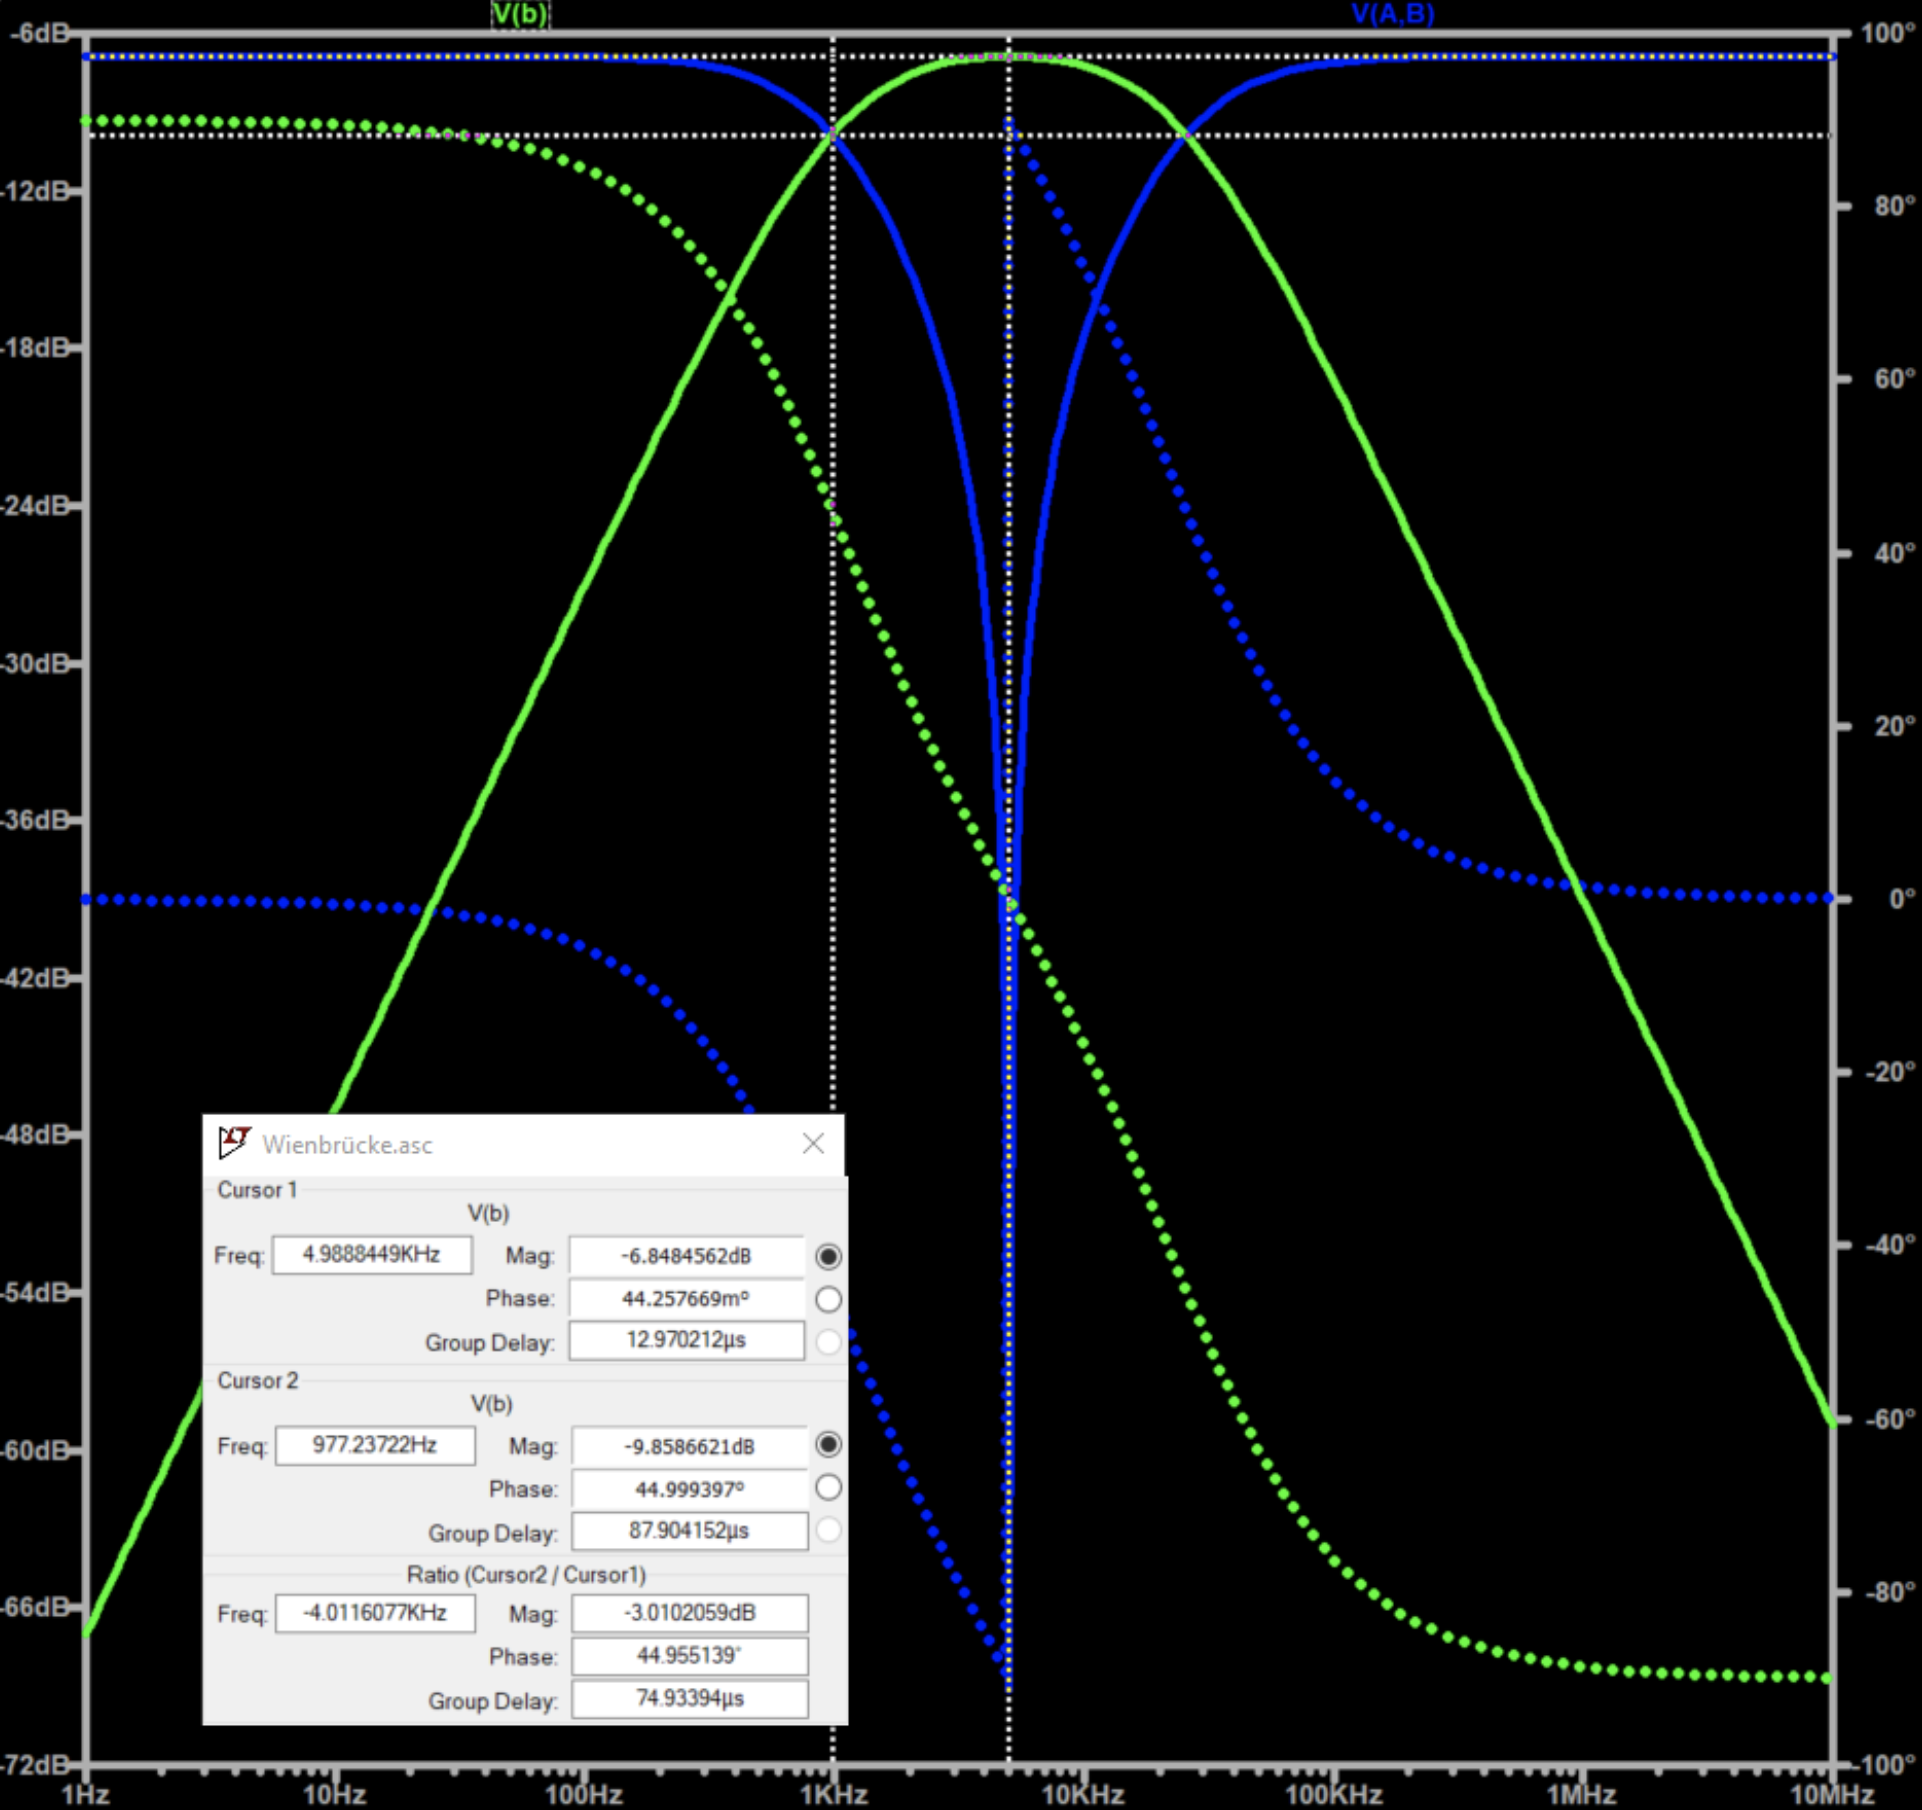
\includegraphics[width=4.5cm]{pictures/Bandsperre.png}}
  \end{figure}

\end{frame}

\begin{frame}[t]{Simulation - Abgleich mit Theorie}

  Bei einer Simulation ist es immer wichtig zu überprüfen, ob das Ergebnis durch eine theoretische Annahme verifiziert werden kann.
  Übernehmen wir nun die untere Grenzfrequenz $f_g=977Hz$ in unsere Spannungsquelle und betrachten nochmals den Zeitbereich über die transiente Simulation.

  \begin{spacing}{0.9} \begin{tiny}
      \begin{minipage}{\textwidth}
        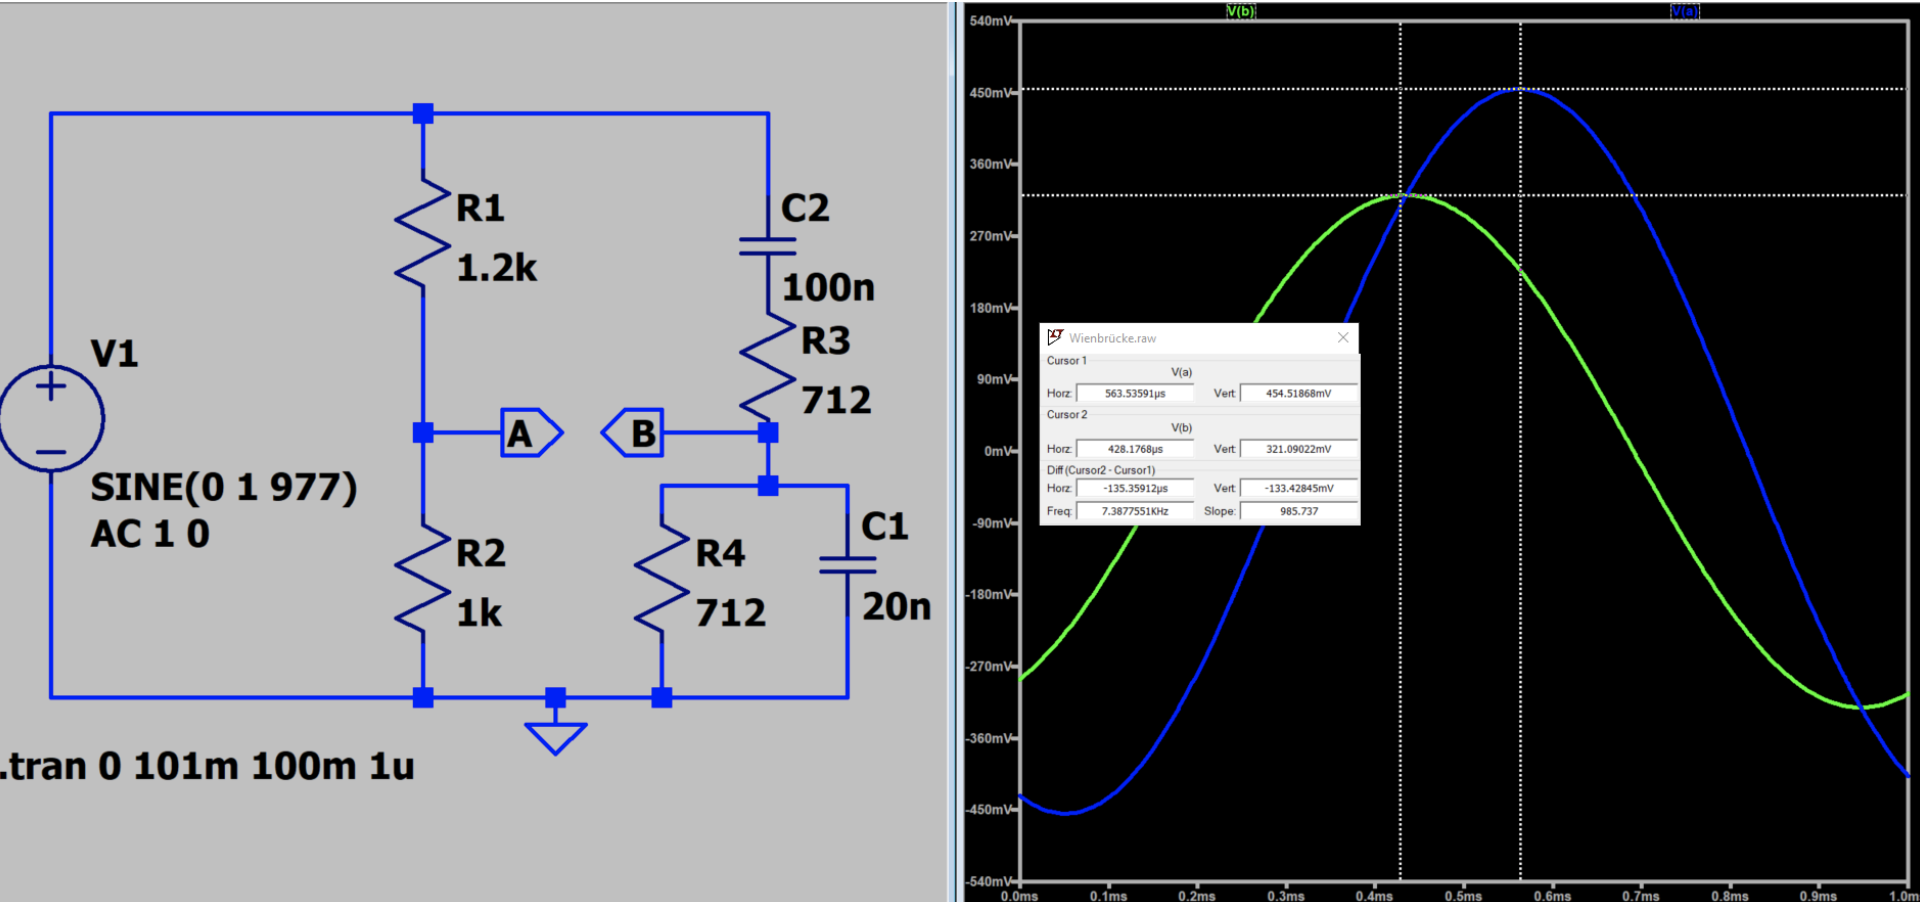
\includegraphics[width=0.75\linewidth]{pictures/wheatstone_transientent_fg.png}
      \end{minipage}
    \end{tiny} \end{spacing}

  \textbf{Das erwartete Verhalten bei der Grenzfrequenz $f_g$ ist, dass die Leistung auf $\frac{1}{\sqrt{2}}$ sinkt.}
\end{frame}

\begin{frame}[t]{Simulation - Abgleich mit Theorie}

  \begin{itemize}
    \item Wir können mittels der Cursor die Spannung $U_A=455mV$ und Spannung $U_B=321mV$ ermitteln.
    \item Dies stimmt mit unserer Erwartungshaltung überein.
  \end{itemize}
  \begin{figure}
    \centering
    $U_B=\frac{455mV}{\sqrt{2}}=321mV$
  \end{figure}

\end{frame}%opv-transient, ac, non inverting

\section{Verwendung \& Modellierung realer Bauteile}

\begin{frame}[t]{Reale Bauteile modellieren}

    LTSpice ist eine wunderbare Simulationsumgebung, allerdings ist die Standardbibliothek
    auf die hauseigenen Bauteile von Linear Technology begrenzt.

    Oftmals ist es jedoch notwending in einer Simulation ein Bauteil zu verwenden,
    das einfach verfügbar ist. Als Beispiel dafür möchten wir gerne einen TS912 modellieren.
    Dieser Operationsverstärker ist leicht beschaffbar und günstig.

    \textbf{Dazu gehen wir in 3 Schritten vor:}

    \begin{enumerate}
        \item Wir suchen im Internet nach dem \textbf{spice model} eines Herstellers
        \item Wir erstellen einen \textbf{subcircuit} in unserer LTSpice Bibliothek
        \item Wir erstellen ein LTSpice \textbf{Symbol}
    \end{enumerate}
\end{frame}


\begin{frame}[t]{TS912 - Recherche} 

    Eine einfache Recherche für uns zu einem Hersteller, hier zum Beispiel ST.
    \href{https://www.st.com/en/amplifiers-and-comparators/ts912.html}{https://www.st.com/en/amplifiers-and-comparators/ts912.html}


    \begin{spacing}{0.9} \begin{tiny}
        \begin{table}[h!]
          \begin{tabular}{p{5cm} p{5cm}}
              \begin{minipage}{0.5\textwidth}
                  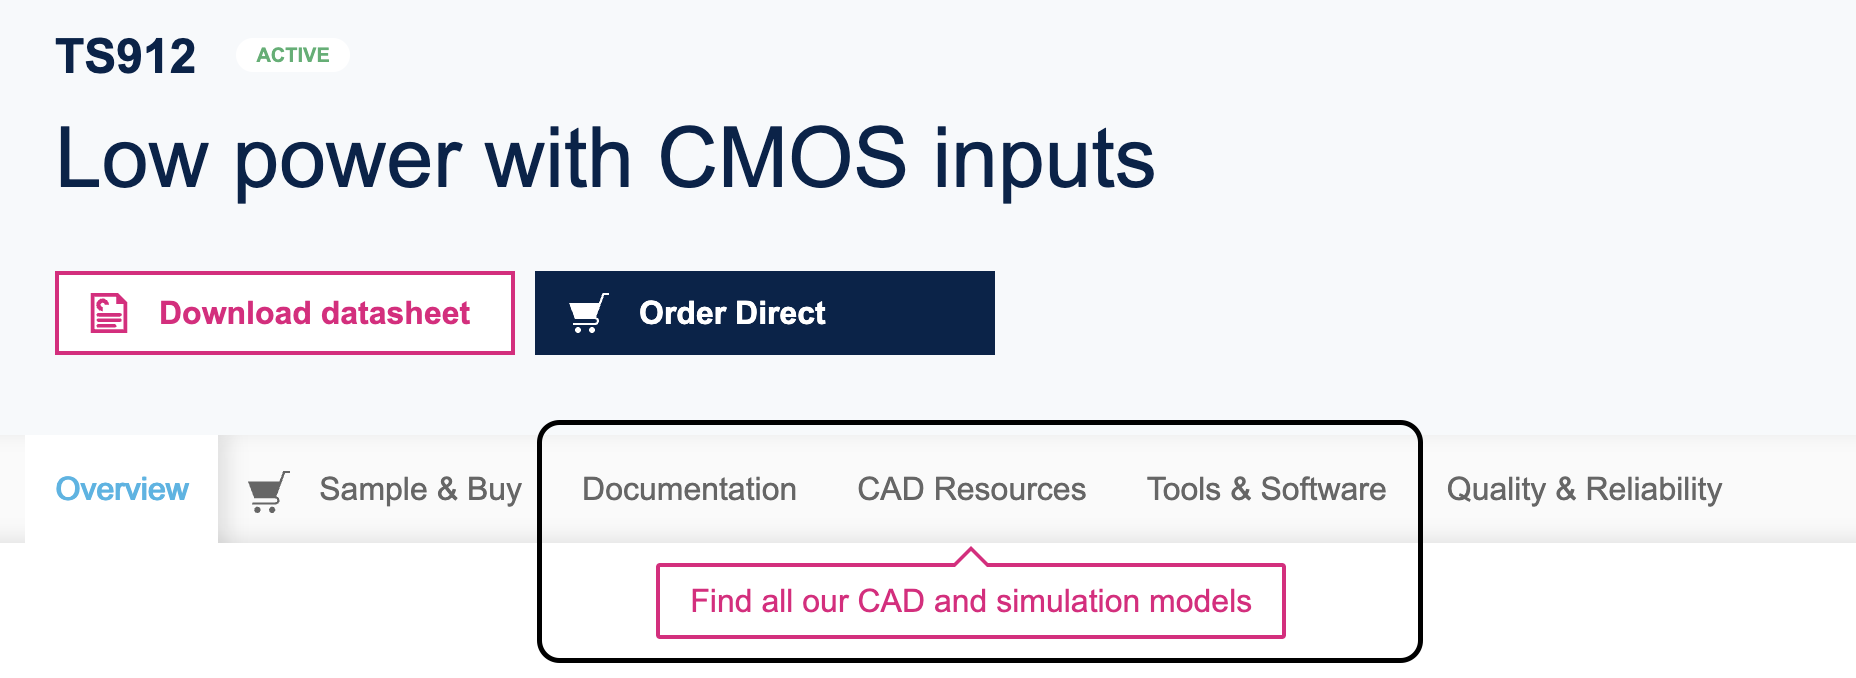
\includegraphics[width=\linewidth]{pictures/spice_model_search.png}
              \end{minipage} 
              &
              \begin{minipage}{0.5\textwidth}
                  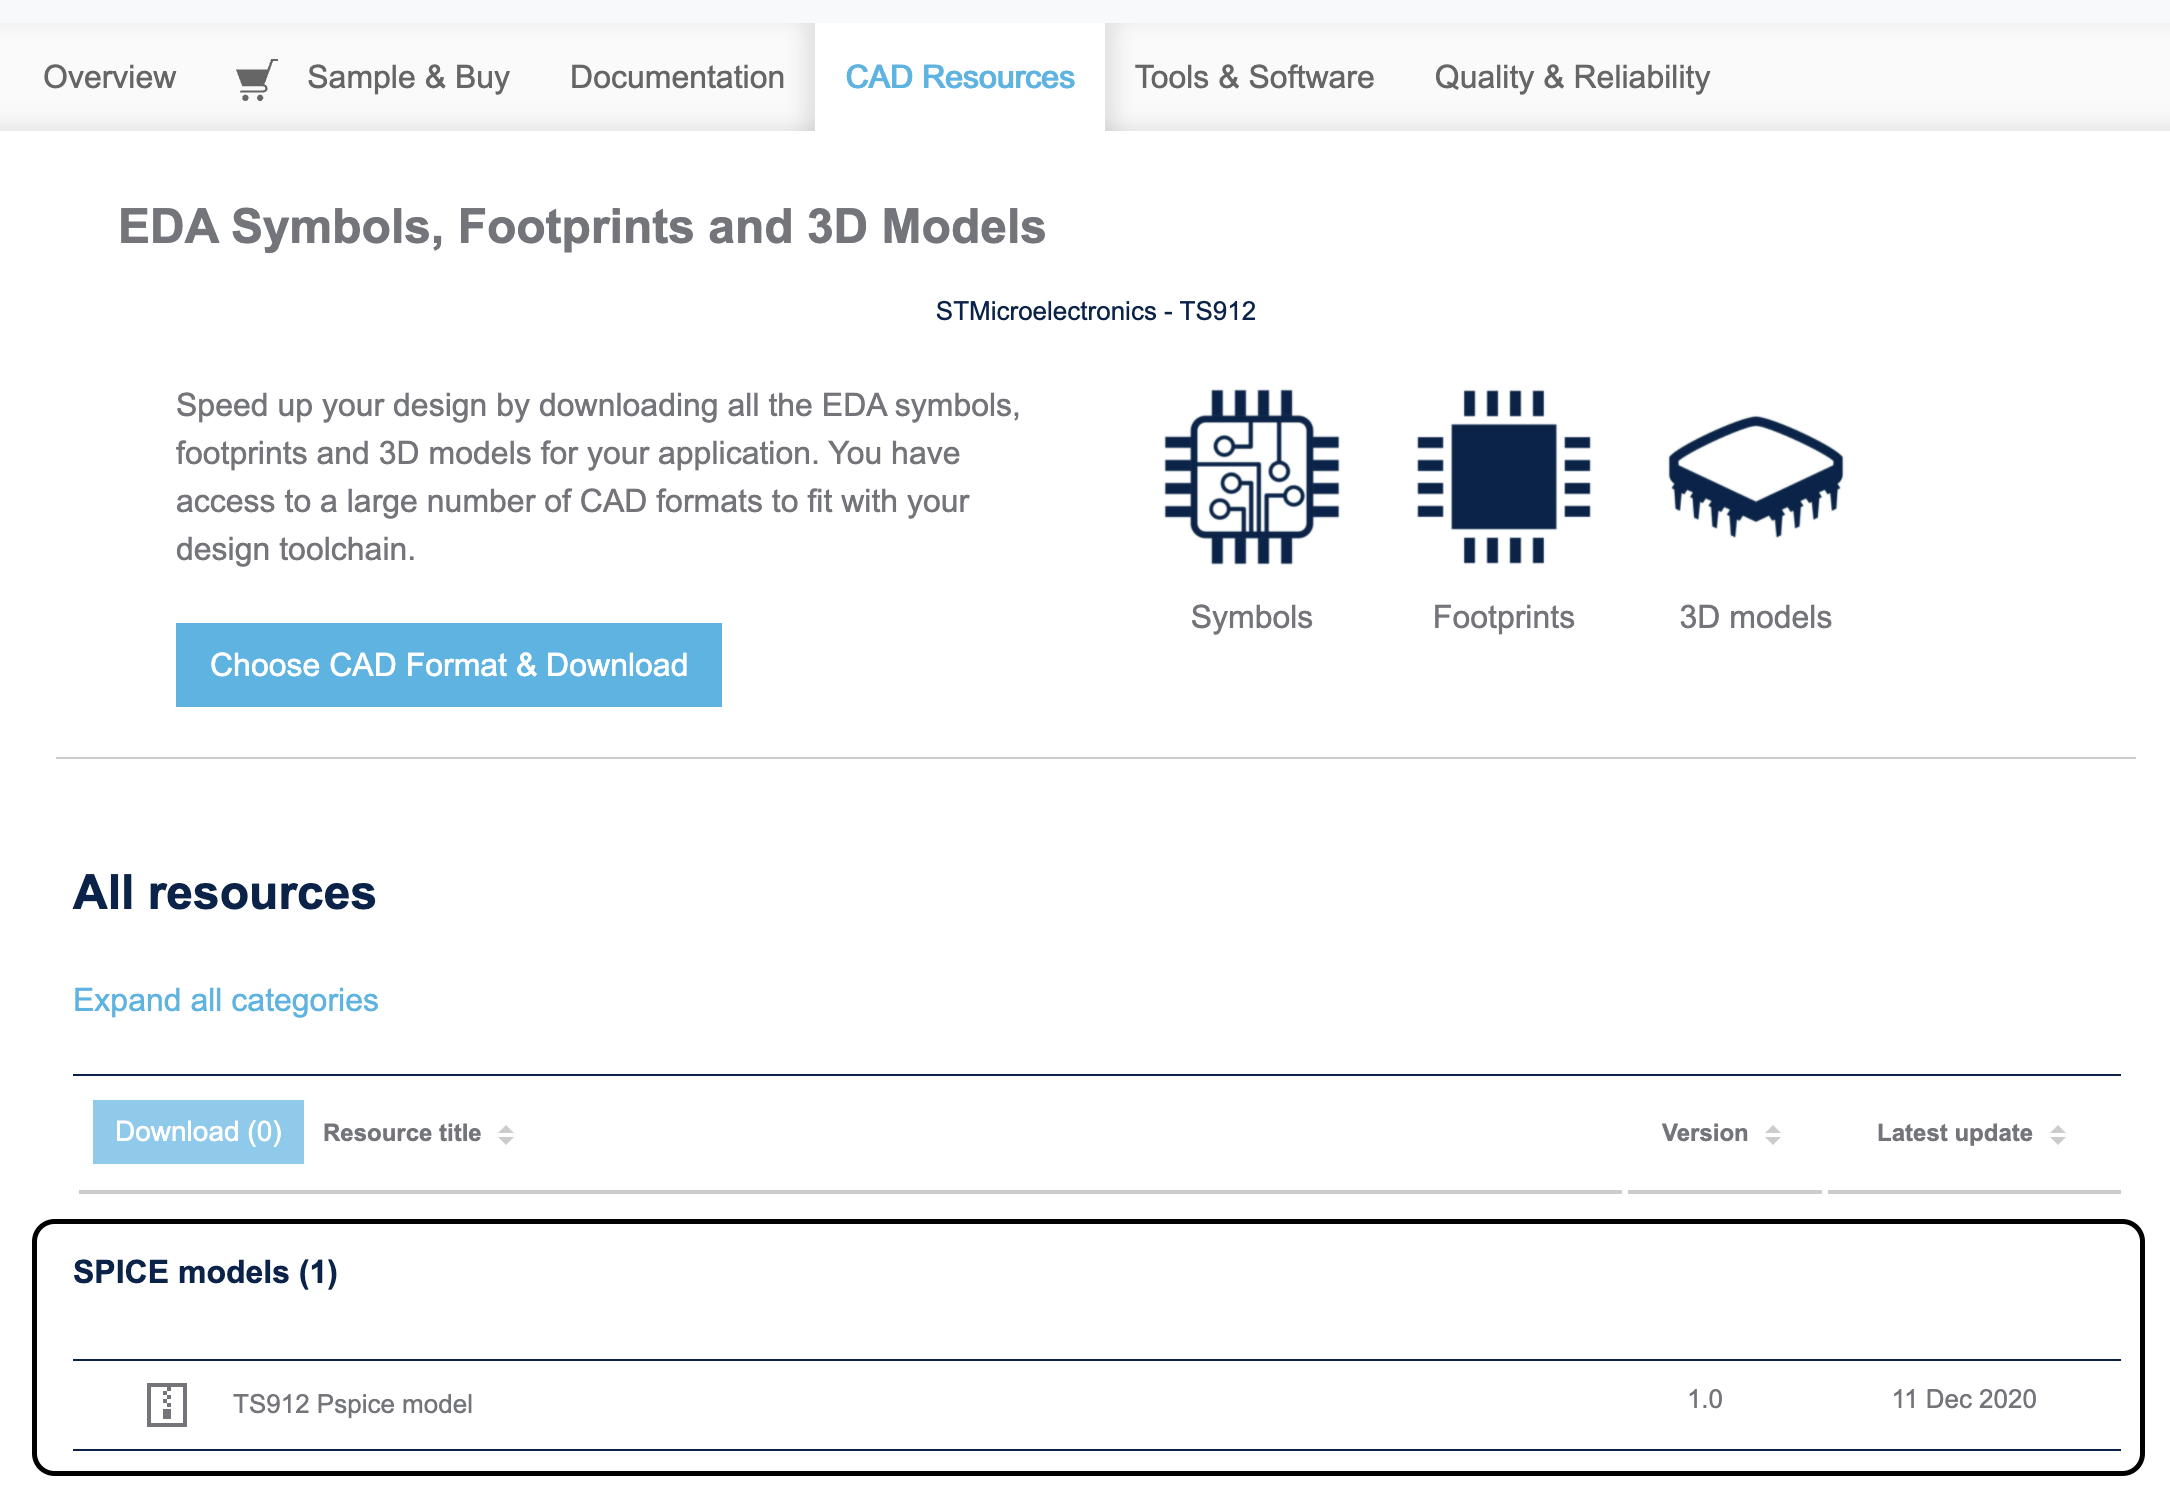
\includegraphics[width=\linewidth]{pictures/spice_model_search2.png}
              \end{minipage} 
        \end{tabular}
      \end{table}
      \end{tiny} \end{spacing}

\end{frame}

\begin{frame}[t]{Subscircuit erstellen} 

    Ein spice Model ist eine einfache Text-Datei, die einfach in LTSpice eingebunden werden kann.
    Kopiert den \textbf{subcircuit} dazu in eine Text-Datei mit der Endung .sub \textbf{ts912.sub} und speichert diese im Ordner:

    \begin{scriptsize}
        \begin{enumerate}
            \item Windows \textbf{LTSpice / lib / sub} 
            \item MacOS \textbf{/Users/"user"/Library/ApplicationSupport/LTspice/lib/sub}.
        \end{enumerate}
    \end{scriptsize}

    \begin{spacing}{0.9} \begin{tiny}
        \begin{minipage}{\textwidth}
          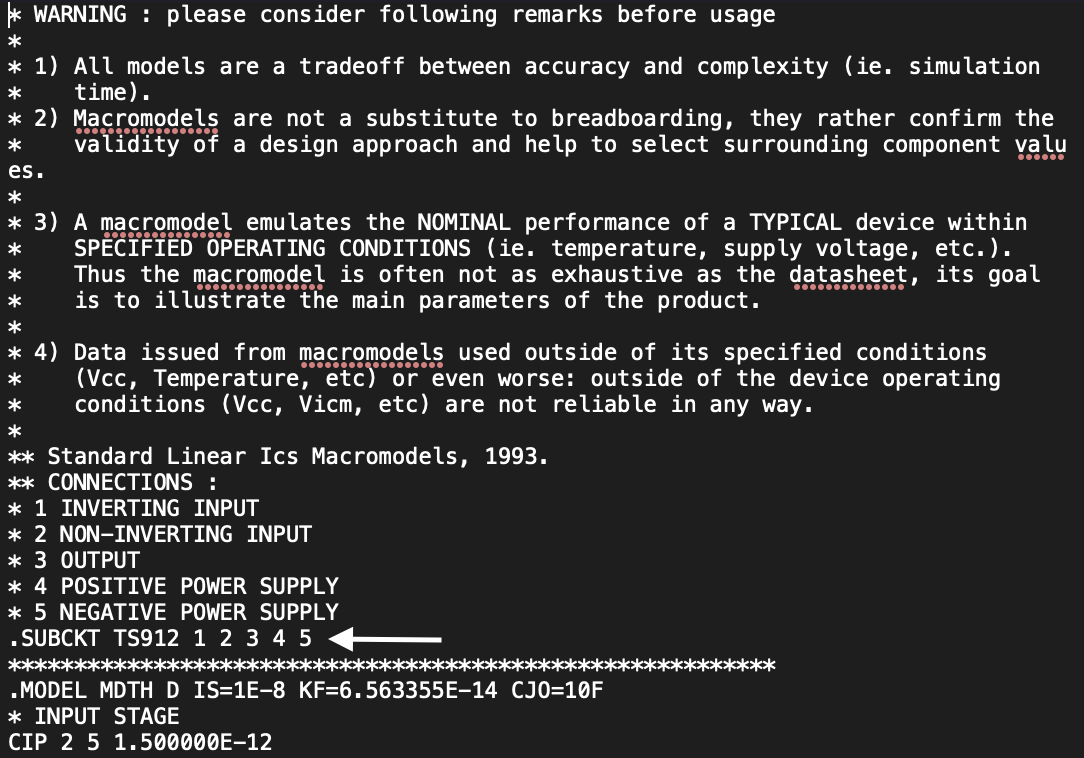
\includegraphics[width=0.5\linewidth]{pictures/spice_model.png}
        \end{minipage}
    \end{tiny} \end{spacing}
\end{frame}

\begin{frame}[t]{LTSpice Symbol erstellen} 

    ...
\end{frame}

\begin{frame}[t]{Bauteil verwenden} 

    ...
\end{frame}

\section{Projekt - Temperaturmessbrücke}

\begin{frame}[t]{Überblick}

    \begin{spacing}{0.9} \begin{tiny}
            \begin{minipage}{\textwidth}
                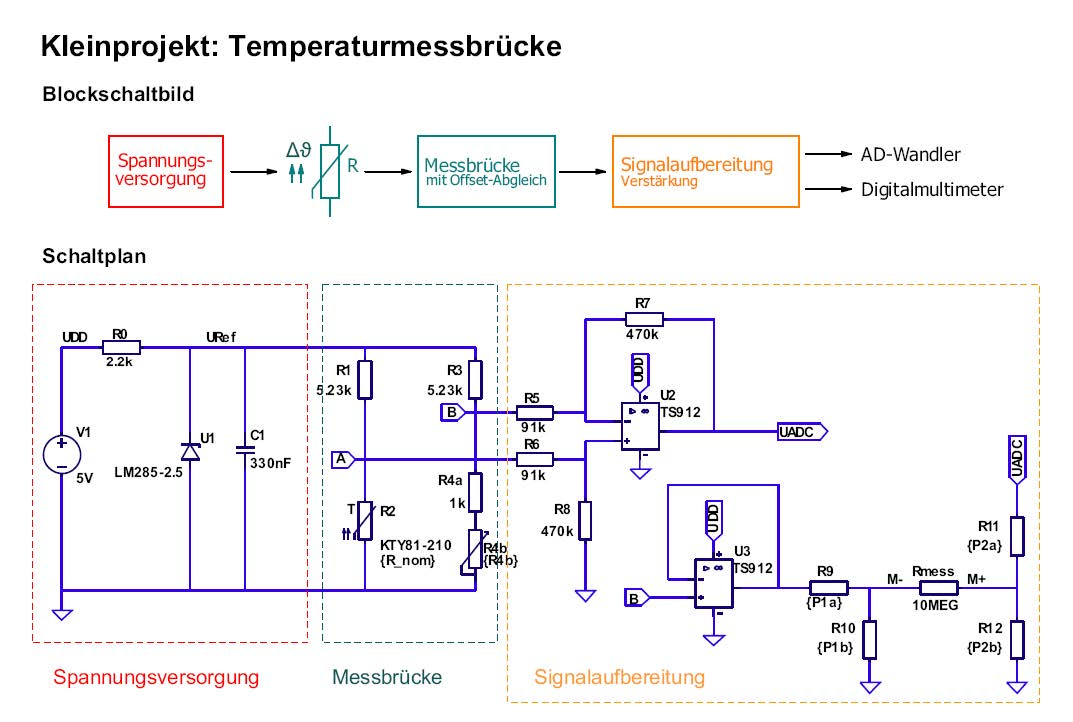
\includegraphics[width=\linewidth]{pictures/projekt_overview.jpg}
            \end{minipage}
        \end{tiny} \end{spacing}

\end{frame}

\begin{frame}[t]{Vorgehenhensweise}

    Zu diesem Zeitpunkt sollten wir alle in der Lage sein einfache Simulationen in DC-,AC-Sweep sowie transient
    durchführen zu können. Sie sollten den Bauteileditor sowie die grundlegenden Schematic-Funktionen (Rotate, Cut, \dots)
    sicher beherrschen.

    Wir werden nun die Bruecke und dir vorgestellten Bestandteile Stück für Stück aufbauen.
    \textbf{Bitte beachtet Folgendes:}

    \begin{enumerate}
        \item Bitte speichert alle Zwischenschritte ab, wir werden Teile später wiederverwenden
        \item Bei Fragen bitten wir euch uns direkt im MS Teams zu benachrichtigen, sodass wir euren
              Fortschritt so gut wie möglich unterstützen können.
    \end{enumerate}
\end{frame}
 % einleitung ins projekt

\begin{frame}[t]{Die Messbrücke - Arbeitspunktanalyse}


  Die Grundlage für unsere Messbruecke bildet eine einfache Wheatstonesche Brueckenschaltung.
  Zur Wiederholung findet ihr unten den Schaltplan sowie die Formel zur Berechnung
  der Brueckenspannung. $V_{AB}$.


  \begin{table}[h!]
    \begin{tabular}{p{5cm} p{5cm}}
      \begin{minipage}{.5\textwidth}
        \begin{figure}
          \scalebox{0.6}{
            \centering
            \begin{circuitikz}
              \ctikzset{bipoles/thickness=1}
              \ctikzset{bipoles/length=.6cm}
              \draw
              (0,0) to [short, *-] (4,0)
              (0,0) to [V, l_=$V_{1}$] (0,-4)
              (2,0) to (2,-0.5)
              (4,0) to (4,-0.5)
              (2,-0.5) to [R, l_=$R_{1}$] (2,-1.5)
              (2,-2.5) to [R, l_=$R_{2}$] (2,-3.5)
              (2,-1.5) to (2,-2.5)
              (2,-2) to [short,*-o] (2.25,-2) node[right]{$V_{a}$}
              (4,-1.5) to (4,-2.5)
              (4,-2) to [short,*-o] (4.25,-2) node[right]{$V_{b}$}
              (4,-0.5) to [R, l_=$R_{3}$] (4,-1.5)
              (4,-2.5) to [R, l_=$R_{4}$] (4,-3.5)
              (2,-3.5) to (2,-4)
              (4,-3.5) to (4,-4)
              (0,-4) node[ground]{}
              (2,-4) node[ground]{}
              (4,-4) node[ground]{}
              ;
            \end{circuitikz}
          }

        \end{figure}
      \end{minipage}
       &

      \begin{spacing}{0.9} \begin{tiny}
          \begin{minipage}{.5\textwidth}
            \begin{equation}
              V_{AB}=\frac{R_2R_3-R_4R_1}{(R_1+R_2)(R_3+R_4)}V_{1}
            \end{equation}
          \end{minipage}
        \end{tiny} \end{spacing}
    \end{tabular}

  \end{table}

\end{frame}



\begin{frame}[t]{Die Messbrücke - Arbeitspunktanalyse}

  \begin{spacing}{0.9} \begin{tiny}
      \begin{table}[h!]
        \begin{tabular}{p{3cm} p{7cm}}
          \hline
          \textbf{Simulation}           & \\
          \hline                          \\
          \begin{minipage}{.3\textwidth}
            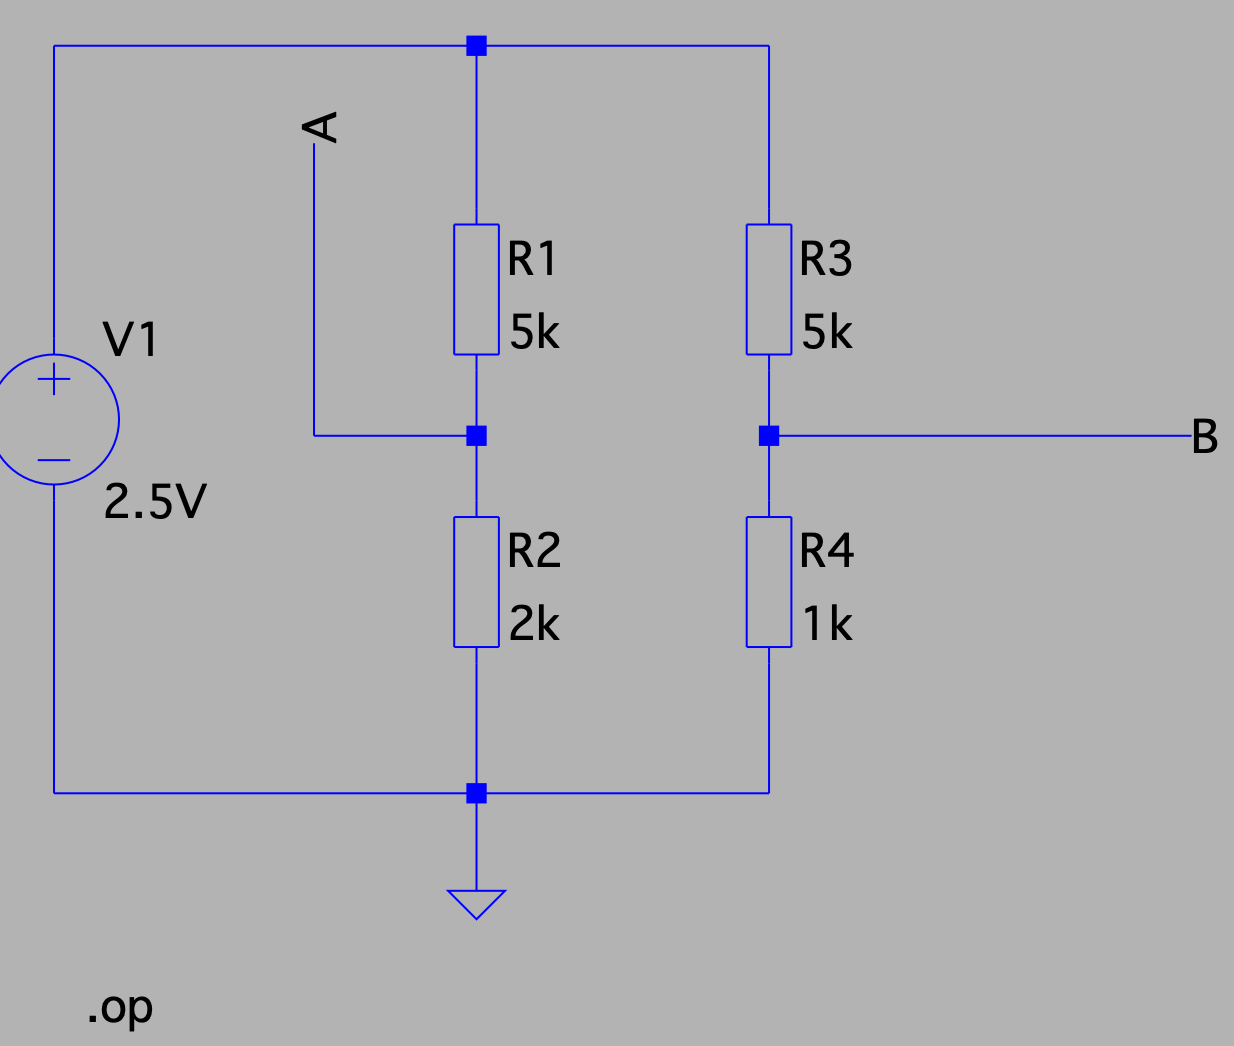
\includegraphics[width=\linewidth]{pictures/bridge_op_2.png}
          \end{minipage}
                                        &
          \begin{minipage}{.7\textwidth}
            \begin{itemize}
              \item Ihr baut die Brueckenschaltung entsprechend auf und verdrahtet Sie
              \item Wir wählen eine neue Analyseart, die Arbeitspunktanalyse \newline(.op == operation point)
              \item Ihr fügt .op als spice-Direktive hinzu \newline(oder wählt im simulation cmd DC Bias Point)
              \item Ihr klickt auf 
\includegraphics[scale=0.3]{pictures/run.png} (run)
            \end{itemize}
          \end{minipage}
          \\
                                        & \\
          \hline
          \textbf{Exkurs zur Netzliste} & \\
          \hline                          \\
          \begin{minipage}{.3\textwidth}
            \includegraphics[width=\linewidth]{pictures/netlist.png}\newline
            \includegraphics[width=\linewidth]{pictures/knotenname.png}
          \end{minipage}
                                        &
          \begin{minipage}{.7\textwidth}

            \begin{itemize}
              \item Der Spice Algorithmus mit einer Netzliste.
              \item Jeder Knoten im Schaltplan erhält einen Namen.
              \item Ihr könnt euch diese Netzliste per\newline rechtem Mausklick $->$ View $->$ SPICE Netlist anzeigen lassen.
              \item Die Masse hat immer den Knotennamen \textbf{0}
              \item Wird ein Knoten \textbf{nicht explizit} mit einem \textbf{Label (F4)} versehen, numeriert LTspice sie aufsteigend durch (N001, N002, \dots)
              \item Weiterhin folgt eine Reihe in der Netzliste dem Schema\newline $<$Bauteil$>$ $<$Knoten1$>$ $<$Knoten2$>$ $<$Bauteilwert$>$
              \item z.B. Widerstand R2 geht von Knoten \textbf{A} (wir haben ein Label vergeben) zur Knoten \textbf{0} (Masse)
              \item Wenn ihr mit der Maus über einen Knoten fahrt, wird euch unten links der Name des Knotens angezeigt.
            \end{itemize}
          \end{minipage}
          \\
        \end{tabular}
      \end{table}
    \end{tiny} \end{spacing}


\end{frame}

\begin{frame}[t]{Die Messbrücke - Arbeitspunktanalyse}

  \begin{spacing}{0.9} \begin{tiny}
      \begin{table}[h!]
        \begin{tabular}{p{3cm} p{7cm}}
          \hline
          \textbf{Analyse der Spannungswerte} & \\
          \hline                                \\
          \begin{minipage}{.3\textwidth}
            \includegraphics[width=\linewidth]{pictures/log_1.png}
          \end{minipage}
                                              &
          \begin{minipage}{.7\textwidth}

            Um die Spannungswerte abzulesen habt mehrere Möglichkeiten.
            \begin{itemize}
              \item Ihr könnt euch den log anzeigen lassen - er sollte direkt bei Start der Analyse erscheinen
              \item Ihr könnt \textbf{nach der Simulation} den gewünschten Knoten \textbf{zweimal} anklicken
              \item \textbf{V(KNOTENNAME)} beschreib das Potential an einem Knoten
              \item \textbf{I(BAUTEILNAME)} beschreibt den Strom durch ein Bauteil hindurch
              \item Per rechtem Mausklick auf einen Wert, öffnet sich ein Dialog über den ihr den Wert frei wählen könnt.
            \end{itemize}
          \end{minipage}
          \\
                                              & \\
          \begin{minipage}{.3\textwidth}
            \includegraphics[width=\linewidth]{pictures/bridge_op_1.png}
          \end{minipage}
                                              &
          \begin{minipage}{.7\textwidth}
            Unter Verwendung der Potentiale und Ströme könnt ihr auch Formeln wie z.B. die Verlustleistung über einem Bauteil
            anzeigen. Per rechtem Mausklick auf einen Knotenspannungswert kommt ihr in das Display Data Menü.
            \begin{figure}
              \centering
              \includegraphics[width=0.8\linewidth]{pictures/manipulation.png}
            \end{figure}
          \end{minipage}
          \\
        \end{tabular}
      \end{table}
    \end{tiny} \end{spacing}


\end{frame}

 % Brückenschaltung und OP analyse
\begin{frame}[t]{Die Messbruecke - Modellierung eines variablen Widerstandes} 
    
    \begin{spacing}{0.9} \begin{tiny}
      \begin{table}[h!]
      \begin{tabular}{p{10cm}}
        \hline
        \textbf{Das Messprinzip} \\
        \hline \\
        \begin{minipage}{\textwidth}

            Ist eine Messbruecke abgegleichen, so gilt:
            \begin{equation}
                \frac{R_1}{R_2} = \frac{R_3}{R_4} 
            \end{equation}
            \begin{equation}
                V_{AB} = 0
            \end{equation}
            Um die Temperatur messen zu können, ersetzen wir den Widerstand $R_2$ durch einen PTC.\newline
            Verändert sich der $R_2$ ist die Brücke nicht mehr abgegleichen und die Spannung $V_{AB}$ ungleich 0.
            \begin{figure}
                \scalebox{0.6}{
              \centering
              \begin{circuitikz}
                \ctikzset{bipoles/thickness=1}
                \ctikzset{bipoles/length=.6cm}
                \draw
                (0,0) to [short, *-] (4,0)
                (0,0) to [V, l_=$V_{1}$] (0,-4)
                (2,0) to (2,-0.5) 
                (4,0) to (4,-0.5) 
                (2,-0.5) to [R, l_=$R_{1}$] (2,-1.5);
                \ctikzset{resistors/fill=red}
                \draw
                (2,-2.5) to [thRp, l_=$R_{2}$] (2,-3.5);
                \ctikzset{resistors/fill=none}
                \draw 
                (2,-1.5) to (2,-2.5) 
                (2,-2) to [short,*-o] (2.25,-2) node[right]{$V_{a}$}
                (4,-1.5) to (4,-2.5) 
                (4,-2) to [short,*-o] (4.25,-2) node[right]{$V_{b}$}
                (4,-0.5) to [R, l_=$R_{3}$] (4,-1.5) 
                (4,-2.5) to [R, l_=$R_{4}$] (4,-3.5) 
                (2,-3.5) to (2,-4) 
                (4,-3.5) to (4,-4) 
                (0,-4) node[ground]{}
                (2,-4) node[ground]{}
                (4,-4) node[ground]{}
                ;
                \end{circuitikz} 
                }
                
            \end{figure}
            Um dieses Prinzip zu simulieren werden wir nun in LTspice den Widerstand $R_2$ modellieren und variieren.
        \end{minipage} 
        \\
      \end{tabular}

    \end{table}
     
    \end{tiny} \end{spacing}

\end{frame}

\begin{frame}[t]{Die Messbruecke - Modellierung eines variablen Widerstandes} 
    
    \begin{spacing}{0.9} \begin{tiny}
      \begin{table}[h!]
      \begin{tabular}{p{10cm}}
        \hline
        \textbf{Ansatz} \\
        \hline \\
        \begin{minipage}{\textwidth}
            \begin{itemize}
                \item Der Widerstand soll durch einen PTC ersetzt werden
                \item Wir nehmen zunächst vereinfacht an, dass sich der Widerstand zwischen 0$°$C - 100$°$C von 1.5k$\Omega$ linear auf 3.5k$\Omega$ erhöht. 
            \end{itemize}
        \end{minipage} 
        \\
        \\
        \hline
        \textbf{Variablen in LTspice} \\
        \hline \\
        \begin{minipage}{\textwidth}
            \begin{figure}
                \centering
                \includegraphics[width=0.45\linewidth]{pictures/rt_var.png}
            \end{figure}
        \end{minipage} 
        \\
      \end{tabular}

    \end{table}
     
    \end{tiny} \end{spacing}

\end{frame}

\begin{frame}[t]{Die Messbruecke - Modellierung eines variablen Widerstandes} 
    \begin{spacing}{0.9} \begin{tiny}
      \begin{table}[h!]
      \begin{tabular}{p{3cm} p{7cm}}
        \hline
        \textbf{Definition von Variablen} \\
        \hline \\
        \begin{minipage}{.3\textwidth}
            \begin{figure}
                \centering
                \includegraphics[width=0.9\linewidth]{pictures/step_param.png}
            \end{figure}
          \end{minipage} 
          & 
          \begin{minipage}{.7\textwidth}
            Variablen können auf verschiedene Weisen variiert werden.\newline 
            \begin{itemize}
                \item Eine Möglichkeit ist die spice-Direktive $.step\ param$
                \item Fügt einfach eine spice-Direktive hinzu\newline (Edit $->$ Spice Directive (\textbf{oder drückt S}))
                \item $.step\ param\ <varname> <start> <stop> <step>$
            \end{itemize}
          \end{minipage} 
          \\
      \end{tabular}
        \\      
      \begin{tabular}{p{5cm} p{5cm}}
        \hline
        \textbf{Simulieren in Abhängigkeit von RT} \\
        \hline \\
        \begin{minipage}{0.5\textwidth}
            \begin{figure}
                \centering
                \includegraphics[width=0.9\linewidth]{pictures/rt_analysis_1.png}
                \includegraphics[width=0.9\linewidth]{pictures/rt_analysis_3.png}
            \end{figure}
        \end{minipage} 
        &
        \begin{minipage}{0.5\textwidth}
            \begin{itemize}
                \item Es wird die \textbf{Spannung} über dem variablen Widerstand auf der x-Achse aufgetragen
                \item Ihr könnt die Spannung zwischen den $A$ und $B$ anzeigen lassen:
                \item ... über den waveform viewer $->$ add traces $->$ V(A,B) (Spannung von Knoten zu Knoten)
                \item ... im schematic, indem ihr mit der roten Messpitze (\includegraphics[scale=0.1]{pictures/rot.png}) auf ein Potential klickt,
                \item ...... die linke Maustaste gedrückt haltet und mit der erscheinenden schwarzen Messpitze (\includegraphics[scale=0.1]{pictures/black.png}) auf der zweite Potential klickt.
                \item Der \textbf{Strom} kann angezeigt werden, indem ihr mit der Maus über ein Bauteil fahrt und die Strommesszange (\includegraphics[scale=0.1]{pictures/current.png}) anklickt.
                \item Die \textbf{Verlustleistung} kann angezeigt werden, indem ihr mit der Maus über ein Bauteil fahrt, \textbf{Shift} gedrückt haltet und das Temperatursymbol (\includegraphics[scale=0.1]{pictures/power.png}) anklickt.
            \end{itemize}
        \end{minipage} 
        \\
      \end{tabular}

    \end{table}
    \end{tiny} \end{spacing}
\end{frame}

\begin{frame}[t]{Die Messbruecke - Modellierung eines variablen Widerstandes} 
    
    \begin{spacing}{0.9} \begin{tiny}
      \begin{table}[h!]
      \begin{tabular}{p{10cm}}
        \hline
        \textbf{Formeln visualisieren} \\
        \hline \\
        \begin{minipage}{\textwidth}
          Weiterhin könnt ihr im waveform viewer auch beliebige Formlen und somit Kennwerte
          eurer Schaltung berechnen und visualisieren.
            \begin{figure}
                \centering
                \includegraphics[width=0.95\linewidth]{pictures/waveform_formulas.png}
            \end{figure}
            Ihr solltet die folgenden Messwerte der Brückenschaltung ermitteln, bzw. ermittelt haben:
            \begin{itemize}
              \item Brückenspannung $V_{AB}$
              \item Strom durch $I(R_2)$
              \item Verlustleistung $P(R_2)=V_aI(R_2)$
              \item Verifiziert den Widerstandswert $R_2=\frac{V(a)}{I(R_2)}$
            \end{itemize}
        \end{minipage} 
        \\
      \end{tabular}

    \end{table}
     
    \end{tiny} \end{spacing}

\end{frame}
 % Brückenschaltung mit variablen Wiederstand
\begin{frame}[t]{Check - Was haben wir bisher gelernt} 
    \textbf{Bis jetzt solltet ihr die folgenden Elemente beherrschen}
    \begin{itemize}
        \item Verwendung des Bauteileditors (\textbf{F2})
        \item DC-Sweep verstehen und verwenden
        \item Transient verstehen und verwenden
        \item AC-Sweep verstehen und verwenden
        \begin{itemize}
            \item Das Kleinsignal Verhalten einer Spannungsquelle im AC-Sweep verstehen und verwenden
            \item Die Grenzefrequenz einer Filterschaltung simulativ ermitteln 
        \end{itemize}
        \item Eine Arbeitspunktanalyse durchführen
        \item Den waveform viewer verwenden
        \begin{itemize}
            \item traces hinzufügen und anpassen
        \end{itemize}
        \item Variablen im schematic einführen und variieren
        \item Verwendung von Labels (\textbf{F4})
    \end{itemize}
\end{frame} % Brückenschaltung mit variablen Wiederstand
\begin{frame}[t]{Die Messbruecke - realer PTC KTY81-210}

    \begin{spacing}{0.9} \begin{tiny}
            \begin{table}[h!]
                \begin{tabular}{p{10cm}}
                    \hline
                    \textbf{Das Bauteil KTY81-210}    \\
                    \hline                            \\
                    \begin{minipage}{\textwidth}
                        Der KTY81-210 ist ein PTC und wir wollen ihn als Temperaturfühler in unserer Brückenschaltung verwenden.\newline
                        Dazu müssen wir ihn in LTspice modellieren.\newline\newline Um das entsprechende Verhalten nachzubilden benötigen wir die
                        Spezifikation des Sensors aus seinem Datenblatt.
                        \begin{itemize}
                            \item Ihr könnt das Hersteller-Datenblatt hier \href{https://cdn-reichelt.de/documents/datenblatt/B400/KTY81-2\%23PHI.pdf}{ $ << Hyperlink\ zum\ PDF >> $} herunterladen
                            \item Ihr könnt die Hersteller-Formelreferenz hier \href{https://www.mikrocontroller.net/attachment/243481/KTY-Philips.pdf}{$ << Hyperlink\ zum\ PDF >> $} herunterladen
                        \end{itemize}


                    \end{minipage}
                    \\ \\
                    \hline
                    \textbf{Analyse des Datenblattes} \\
                    \hline                            \\
                    \begin{minipage}{\textwidth}
                        Das Datenblatt enthält eine Tabelle die die Widerstandswerte über die Temparatur beschreibt. \newline

                        \begin{tabular}{p{3cm} p{8cm}}
                            \begin{minipage}{.3\textwidth}
                                \includegraphics[width=0.8\linewidth]{pictures/kty81_overview.png}
                                \includegraphics[width=0.8\linewidth]{pictures/kty81_pinning.png}
                                \includegraphics[width=0.8\linewidth]{pictures/kty81_graph.png}
                            \end{minipage}
                             &
                            \begin{minipage}{.7\textwidth}
                                \begin{figure}
                                    \centering
                                    \includegraphics[width=0.45\linewidth]{pictures/kty81_table.png}
                                \end{figure}
                            \end{minipage}
                        \end{tabular}
                    \end{minipage}
                    \\
                \end{tabular}

            \end{table}

        \end{tiny} \end{spacing}

\end{frame}

\begin{frame}[t]{Die Messbruecke - Approximation eines PTC}

    \begin{spacing}{0.9} \begin{tiny}
            \begin{table}[h!]
                \begin{tabular}{p{10cm}}
                    \hline
                    \textbf{Quadratische Approximationsformel} \\
                    \hline                                     \\
                    \begin{minipage}{\textwidth}
                        Der Hersteller gibt in seinem Datenblatt eine Approximationsformel zur Modellierung des Verhaltens an.

                        \begin{equation}
                            R_T=R_{Ref}[1+A(T-T_{Ref})+B(T-T_{Ref})^2+C(T-T_{i}^D)]
                        \end{equation}
                        \begin{figure}
                            \centering
                            \includegraphics[width=0.6\textwidth]{pictures/kty81_constants.png}
                            \includegraphics[width=0.6\textwidth]{pictures/kty81_formula.png}
                        \end{figure}
                    \end{minipage}
                \end{tabular}

            \end{table}

        \end{tiny} \end{spacing}

\end{frame}

\begin{frame}[t]{Die Messbruecke - Approximation eines PTC}

    \begin{spacing}{0.9} \begin{tiny}
            \begin{table}[h!]
                \begin{tabular}{p{10cm}}
                    \hline
                    \textbf{Genauigkeit Approximation} \\
                    \hline                             \\
                    \begin{minipage}{\textwidth}
                        Wenn wir die Tabelle aus dem Datenblatt mit der quadratischen Approximationsformel (Formel 6, $C=0$) vergleichen ergibt sich folgender Verlauf.
                        \begin{figure}
                            \centering
                            \includegraphics[width=0.6\textwidth]{pictures/kty81_approx_accuracy.png}
                        \end{figure}
                        Aus Formel 6 wissen wir, dass die quadratische Approximation ab einer Temparatur $T>T_i$ nicht mehr vollständig ist.
                        Diesen Effekt sehen wir hier. Ab $T>T_i=100$ weicht der reale Verlauf ab. Wenn wir unseren Messbereich jedoch auf -50$°$C - 100$°$C begrenzen, können
                        wir die quadratische Formel verwenden. \newline\newline Dies werden wir im nächsten Schritt tun.
                    \end{minipage}
                \end{tabular}

            \end{table}

        \end{tiny} \end{spacing}

\end{frame}

\begin{frame}[t]{Die Messbruecke - Modellierung des KTY81-210}

    \begin{spacing}{0.9} \begin{tiny}
            \begin{table}[h!]
                \begin{tabular}{p{10cm}}
                    \hline
                    \textbf{Widerstandsformel als Variable} \\
                    \hline                                  \\
                    \begin{minipage}{\textwidth}
                        Zur Modellierung starten wir mit einem einfachen schematic.
                    \end{minipage}
                    \\ \\
                \end{tabular}
                \begin{tabular}{p{3cm} p{7cm}}
                    \begin{minipage}{.3\textwidth}
                        \includegraphics[width=0.8\linewidth]{pictures/kty81_test.png}
                    \end{minipage}
                     &
                    \begin{minipage}{.7\textwidth}
                        \begin{itemize}
                            \item Baut den Schaltplan auf
                            \item Gebt dem Widerstand $R_1$ eine Variable $KTY81-210$ als Wert
                            \item Erstellt ein Label mit dem Namen $KTY81-210$
                        \end{itemize}
                    \end{minipage}
                    \\\\
                \end{tabular}
                \begin{tabular}{p{10cm}}
                    \begin{minipage}{\textwidth}
                        Um den Widerstand abhängig von der Temparatur und seiner Formel zu simulieren gehen wir wie folgt vor:
                        \begin{itemize}
                            \item Schrittweite Steigerung der Temparatur
                            \item Simulation entsprechend Formel 6 mit $R_{Ref}=2k$ $A=7.874^{-3}$ $B=1.874^{-5}$ $T_{Ref}=25$
                            \item $R_{KTY81-210}=2k[1+7.874^{-3}(T-25)+1.874^{-5}(T-25)^2]$
                        \end{itemize}
                    \end{minipage}
                    \\ \\
                \end{tabular}
                \begin{tabular}{p{3cm} p{7cm}}
                    \begin{minipage}{.3\textwidth}
                        \includegraphics[width=0.8\linewidth]{pictures/kty81_simulation.png}
                    \end{minipage}
                     &
                    \begin{minipage}{.7\textwidth}
                        \begin{itemize}
                            \item Ihr könnt für die Variable eine Formel über die Spice-Direktive $.param$ hinterlegen
                            \item Über die Spice-Direktive $.step$ könnt ihr einen Parameter $TEMP1$ (nicht $TEMP$ dieser beschreibt die globale Temparatur) für die Tempartur einführen und variieren.
                            \item In einer Arbeitspunktanalyse können wir uns nun den trace von $R_1=\frac{V(KTY81-210)}{I(R_1)}$ anzeigen lassen.
                        \end{itemize}
                    \end{minipage}
                    \\\\\\
                \end{tabular}
                \begin{tabular}{p{10cm}}
                    \begin{minipage}{\textwidth}
                        \begin{center}
                            \textbf{Entspricht der Verlauf dem des Datenblattes und euren Erwartungen? \newline
                                Wenn ja, dann können wir diesen Widerstand nun in unsere Messbruecke übernehmen.}
                        \end{center}
                    \end{minipage}
                    \\ \\
                \end{tabular}
            \end{table}
        \end{tiny} \end{spacing}

\end{frame} % einführung Kty
\begin{frame}[t]{Die Messbruecke - mit KTY81}

    \begin{spacing}{0.9} \begin{tiny}
            \begin{table}[h!]
                \begin{tabular}{p{5cm} p{5cm} }
                    \hline
                    \textbf{Schaltungsaufbau} \\
                    \hline                    \\
                    \begin{minipage}{0.5\textwidth}
                        \includegraphics[width=0.9\linewidth]{pictures/mb_kty81.png}
                    \end{minipage}
                     &
                    \begin{minipage}{0.5\textwidth}
                        \begin{itemize}
                            \item Ihr baut den KTY81-210 inklusive der als spice-Direktive modellierten Formel in eure Messbreuckenschaltung ein
                            \item Prüft ob das Model immer noch simulierbar ist und es zu keinem Fehler kommt.
                        \end{itemize}
                    \end{minipage}
                    \\
                \end{tabular}

            \end{table}

        \end{tiny} \end{spacing}

\end{frame}

\begin{frame}[t]{Die Messbruecke - Linearisierung der Kennlinie}

    \begin{spacing}{0.9} \begin{tiny}
            \begin{table}[h!]
                \begin{tabular}{p{10cm} }
                    \hline
                    \textbf{Problemstellung}                     \\
                    \hline                                       \\
                    \begin{minipage}{\textwidth}
                        \begin{itemize}
                            \item Die Formel zur Approximation des PTC is quadratisch
                            \item Dadruch sind wird unsere Messung "nicht-linear" und wir werden bei einer \textbf{konstanten Temperaturerhöhrung keine
                                      konstante Spannungserhöhrung} erwarten können
                        \end{itemize}
                    \end{minipage}
                    \\ \\
                    \hline
                    \textbf{Simulatives Experiment}              \\
                    \hline                                       \\
                    \begin{minipage}{\textwidth}
                        Zur Annäherung werden wir die Vorwiderstand R1 ebenfalls variieren, um experimentell einen linearen Verlauf der Spannung $V_{AB}$ zu ermitteln.
                    \end{minipage}
                    \\\\
                    \begin{tabular}{p{5cm} p{5cm}}
                        \begin{minipage}{0.5\textwidth}

                            \begin{figure}
                                \centering
                                \includegraphics[width=0.95\linewidth]{pictures/mb_kty81_steps.png}
                            \end{figure}
                        \end{minipage}
                         &
                        \begin{minipage}{0.5\textwidth}
                            \begin{itemize}
                                \item Variiert den Vorwiderstand $R_1$ als Parameter $R_V$
                                \item Über die Spice-Direktive $.step\ param\ <Var>\ list\ <Wert_1>\ ...\ <Wert_n>$ könnt ihr eine Liste von Werten hinterlegen
                                \item Wir wählen einen Wertebereich von $500\Omega$ - $20k\Omega$
                                \item Positioniniert die Spice-Direktive $.step param Rv$ \textbf{nach} der Temperatur $TEMP1$, da der erste Wert auf der Abzisse dargestellt wird
                                \item Im waveform viewer könnt ihr über $rechter\ Mausklick$ $->$ $View$ $->$ $Steps$ die einzelnen Werte auswählen und eigenständig bewerten.
                            \end{itemize}
                        \end{minipage}
                    \end{tabular}
                    \\\\
                    \hline
                    \textbf{Hinweis zur Simulationsschrittweite} \\
                    \hline                                       \\
                    \begin{minipage}{\textwidth}
                        Wählt die Schrittweite immer möglichst klein, da zu viele Werte die Übersichtlichkeit erschweren!
                    \end{minipage}
                \end{tabular}

            \end{table}

        \end{tiny} \end{spacing}

\end{frame}

\begin{frame}[t]{Die Messbruecke - Linearisierung der Kennlinie}

    \begin{spacing}{0.9} \begin{tiny}
            \begin{table}[h!]
                \begin{tabular}{p{10cm} }
                    \hline
                    \textbf{Analytische Herleitung} \\
                    \hline                          \\
                    \begin{minipage}{\textwidth}
                        Den exakten Wert kann man auch analytisch Herleiten. Dazu schauen wir uns den Spannungsteiler des PTCs genauer an.
                    \end{minipage}
                    \begin{minipage}{\textwidth}
                        \begin{figure}
                            \centering
                            \includegraphics[width=0.9\linewidth]{pictures/linearisierung.png}
                        \end{figure}
                    \end{minipage}
                    \\
                \end{tabular}

            \end{table}

        \end{tiny} \end{spacing}

\end{frame} % linearisierung
\begin{frame}[t]{Die Messbruecke - Abgleich der Messbruecke}

    \begin{spacing}{0.9} \begin{tiny}
            \begin{table}[h!]
                \begin{tabular}{p{10cm} }
                    \hline
                    \textbf{Definition des Messbereichs} \\
                    \hline                               \\
                    \begin{minipage}{\textwidth}
                        \begin{itemize}
                            \item Unsere Temperaturmessbruecke mit einem 8Bit AD-Wandler digitalisiert werden
                            \item 254 Schritte
                            \item quadratische Approximation bis $100$C genau
                            \item wir wählen eine Schrittweite von $0,5$C
                        \end{itemize}
                        Somit ergibt sich ein Temperaturbereich von $-27$C bist $100,5$C und die folgende Anforderung an unser Schaltung.\newline\newline
                        \textbf{Die Messbrücke soll bei $-27$C abgeglichen sein.}
                        \begin{itemize}
                            \item Der KTY81-210 hat laut Datenblatt einen bei -27C Widerstand von $1282\Omega$
                            \item $R_4$ muss daher $1282\Omega$ betragen
                            \item In der Realität würde man einen $1k\Omega$ und einen auf $282\Omega$ getrimmten $500\Omega$-Trimmer verwenden
                            \item In unserer Simulation reicht ein einfacher Widerstand mit $1282\Omega$ aus.
                        \end{itemize}
                        \begin{figure}
                            \includegraphics[width=0.5\linewidth]{pictures/kty81_getrimmet.png}
                        \end{figure}
                    \end{minipage}
                    \\
                \end{tabular}

            \end{table}

        \end{tiny} \end{spacing}

\end{frame}

\begin{frame}[t]{Die Messbruecke - Anpassung an AD-Wandler}

    \begin{spacing}{0.9} \begin{tiny}
            \begin{table}[h!]
                \begin{tabular}{p{10cm} }
                    \hline
                    \textbf{Ausnutzung des Quantisierungsbereiches des AD-Wandlers} \\
                    \hline                                                          \\
                    \begin{minipage}{\textwidth}
                        \begin{itemize}
                            \item Der AD-Wandler hat eine Referenzspannung von 2,5V
                            \item In der vorherigen Folie sehen wir, dass die Spannung der Messbrücke von 0 bis etwa 500mV reicht
                            \item Zur Ausnutzung des kompletten Quantisierungsbereiches des AD-Wandlers muss die Brückenspannung auf 2,5V bei 100,5C verstärkt werden
                        \end{itemize}
                        \textbf{Hierzu werden wir einen Differenzverstärker verwenden}
                    \end{minipage}
                    \\  \\
                    \hline
                    \textbf{Exkurs Differenzverstärker}                             \\
                    \hline                                                          \\
                    \begin{tabular}{p{5cm} p{5cm}}
                        \begin{minipage}{0.5\textwidth}
                            \begin{figure}[h!]
                                \scalebox{0.6}{
                                    \centering
                                    \begin{circuitikz}
                                        \draw
                                        (0, 0) node[op amp] (opamp) {}
                                        (opamp.-) to[R,l=$R_1$] (-3, 0.5) to[short,-*,l=$V_a$] ++ (-1,0)
                                        (opamp.+) to[R,l=$R_2$] (-3, -0.5) to[short,-*,l=$V_b$] ++ (-0.5,0)
                                        (opamp.-) to[short] ++(0,1.5) coordinate (leftR)
                                        to[R,l=$R_k$] (leftR -| opamp.out)
                                        to[short] (opamp.out) to[short,-*,l=$U_{ADC}$] ++ (0.5,0)
                                        (opamp.+) to[R,l=$R_q$] (-1.2,-2) node[ground]{};
                                    \end{circuitikz}
                                }
                            \end{figure}
                        \end{minipage}
                         &
                        \begin{minipage}{0.4\textwidth}
                            Wenn gilt:\newline
                            \begin{equation}
                                V_{D} = \frac{R_k}{R_1} = \frac{R_q}{R_2}
                            \end{equation}
                            Dann ist der Differenzverstärker symmetrisch und kann mit der folgenden Formel dimensioniert werden.\newline
                            \begin{equation}
                                U_{ADC}=V_{D}(V_b-V_a)
                            \end{equation}
                            Um die folgenden Berechnungen zu vereinfachen verwenden wir einen symmetrischen Differenzverstärker.
                        \end{minipage}
                    \end{tabular}
                \end{tabular}

            \end{table}

        \end{tiny} \end{spacing}

\end{frame}

\begin{frame}[t]{Die Messbruecke - Anpassung an AD-Wandler}

    \begin{spacing}{0.9} \begin{tiny}
            \begin{table}[h!]
                \begin{tabular}{p{10cm} }
                    \hline
                    \textbf{Dimensionierung Differenzverstärker}             \\
                    \hline                                                   \\
                    \begin{minipage}{\textwidth}
                        \begin{itemize}
                            \item Aus unserer Simulation (Folie 45) wissen wir, dass die Spannung $V_{AB}$ bei 100C 493mV entspricht
                            \item Die Referenzspannung des AD-Wandler ist 2,5V
                            \item Das ergibt einen Verstärkungsfaktor $V_D=\frac{2,5}{0,493}=\thicksim 5,1$
                            \item Wir wählen daher $R_k=R_q=470k\Omega$ sowie $R_1=R_2=91k\Omega$
                        \end{itemize}
                    \end{minipage}
                    \\\\
                    \hline
                    \textbf{Aufbau des Differenzverstärkers und Integration} \\
                    \hline                                                   \\
                    \begin{minipage}{\textwidth}
                        Zur einfacheren Versorgung (eine 5V Versorgung für alles anstatt einer zusätzlichen +/-12V Versorgung)
                        verwenden wir den UniversalOpamp2 im unsymmetrischen Modus von 5V bis 0V. Dies reicht aus, da unser Messbereich
                        von 0-2,5V reicht.
                        \begin{figure}
                            \centering
                            \includegraphics[width=0.5\linewidth]{pictures/diff_ampl_uadc_1.png}
                        \end{figure}
                    \end{minipage}
                \end{tabular}

            \end{table}

        \end{tiny} \end{spacing}

\end{frame}

\begin{frame}[t]{Die Messbruecke - Alternative Anzeige am Digitalmultimeter}

    \begin{spacing}{0.9} \begin{tiny}
            \begin{table}[h!]
                \begin{tabular}{p{10cm} }
                    \hline
                    \textbf{Potentailanpassung für das Multimeter} \\
                    \hline                                         \\
                    \begin{minipage}{\textwidth}
                        Alternativ kann die Spannung direkt an einem Digitalmultimeter angezeigt werden. \newline
                        Das Digitalmultimeter soll jedoch idealerweise direkt die Temperatur ohne Umrechnungsfaktor anzeigen.
                        \textbf{Wir haben einen nahezu idealen unsymmetrischen OPVs verwendet. Hier sehen wir, dass (wie auch bei einem realen TS912-5) die Kurve am Beginn des Messbereichs leicht abflacht. Daher limitieren wir den Messbreich bei -20C.}
                        \begin{figure}
                            \centering
                            \includegraphics[width=0.4\linewidth]{pictures/digimul_ready.png}
                        \end{figure}
                        Um die Anpassung durchzuführen werden wir die folgenden Schritte abarbeiten um die Spannung der Temperatur anzugleichen:
                        \begin{itemize}
                            \item Spannungsteiler reduziert das Potential $U_{ADC}$
                            \item Wir nutzen die temperaturkonstante Spannung $V_B$ mit einem weiteren Spannungsteiler um das Potential am negativen Messpunkt um 270mV zu senken
                            \item \textbf{Für die Spannungsteiler müssen Potis zur initialen Einstellung verwendet werden, da es keine Widerstände in beliebigen Werten gibt. Jedenfalls nicht um unsere Spannungsteiler exakt zu dimensionieren.}
                        \end{itemize}
                    \end{minipage}
                \end{tabular}

            \end{table}

        \end{tiny} \end{spacing}

\end{frame}

\begin{frame}[t]{Die Messbruecke - Alternative Anzeige am Digitalmultimeter}

    \begin{spacing}{0.9} \begin{tiny}
            \begin{table}[h!]
                \begin{tabular}{p{10cm} }
                    \hline
                    \textbf{Schematic mit Modellierung von Potis} \\
                    \hline                                        \\
                    \begin{minipage}{\textwidth}
                        \begin{itemize}
                            \item Spannungsteiler $U_{UAC} \frac{1,27}{2,5}=\thicksim 0,51$
                            \item $U_{B}=2,5(\frac{5,23k\Omega}{1,28k\Omega+5,23k\Omega})=0,492V=konstant$
                            \item Spannungsteiler $U_{B}=\frac{0,27}{0,492}=\thicksim 0,54$
                            \item $R_{Mess}$ sollte möglichst hochohmig dimensioniert werden.
                        \end{itemize}
                        \begin{figure}
                            \centering
                            \includegraphics[width=0.7\linewidth]{pictures/digi_mul_anpassung_2.png}
                        \end{figure}
                    \end{minipage}
                \end{tabular}

            \end{table}

        \end{tiny} \end{spacing}

\end{frame}

\begin{frame}[t]{Die Messbruecke - Die Referenzspannungsquelle}

    \begin{spacing}{0.9} \begin{tiny}
            \begin{table}[h!]
                \begin{tabular}{p{10cm} }
                    \hline
                    \textbf{Verwendung eines realen Bauelementes} \\
                    \hline                                        \\
                    \begin{minipage}{\textwidth}
                        Beim praktischen Schaltungsaufbau lässt sich die Referenzspannung mit einer Referenzdiode (z.B. direkt von analog devices ADR4525)
                        aus der Versorgungsspannung erzeugen. \textbf{Wir haben hier bisher eine ideale Spannungsquelle in der Simulation verwendet!}\newline
                        \begin{figure}
                            \includegraphics[width=0.8\linewidth]{pictures/uref.png}
                        \end{figure}
                        Im Vergleich zur Übersicht auf Folie 28, ist der LM285-2.5 nicht mehr in der Bauteilbibliothek verfügbar.
                        Daher haben wir hier zur realen Modellierung der Spannungsversorgung ein Bauteil von analog devices verwendet.
                    \end{minipage}
                \end{tabular}

            \end{table}

        \end{tiny} \end{spacing}

\end{frame}

\begin{frame}[t]{Die Messbruecke - Alles zusammen}

    \begin{spacing}{0.9} \begin{tiny}
            \begin{table}[h!]
                \begin{tabular}{p{10cm} }
                    \hline
                    \textbf{-0,2 bis 1V bei Abgriff von M+ nach M-} \\
                    \hline                                          \\
                    \begin{minipage}{\textwidth}
                        \begin{figure}
                            \includegraphics[width=\linewidth]{pictures/complete_2.png}
                        \end{figure}
                    \end{minipage}
                \end{tabular}

            \end{table}

        \end{tiny} \end{spacing}

\end{frame} % differenzenverstärker

\section{Appendix}

\begin{frame}[t]{Reale Bauteile modellieren mit einem subcircuit} 
    
    \begin{spacing}{0.9} \begin{tiny}
      \begin{table}[h!]
        \begin{tabular}{p{5cm} p{5cm}}
            \begin{minipage}{0.5\textwidth}
                Hier findet ihr eine Übersicht wie man ein reales Bauteil im Internet findet,
                den subcircuit einbindet und ein Modellfile dazu erzeugt. Diese Dateien sind Übernahmen
                aus dem alten Skript CAE Labor von Franz Smagacz-Allramseder. \newline

                \includegraphics[width=\linewidth]{pictures/legacy/tl072_1.png}
            \end{minipage} 
            &
            \begin{minipage}{0.5\textwidth}
                \includegraphics[width=\linewidth]{pictures/legacy/tl072_2.png}
            \end{minipage} 
      \end{tabular}
    \end{table}
    \end{tiny} \end{spacing}
\end{frame}

\begin{frame}[t]{Reale Bauteile modellieren mit einem subcircuit} 
    
    \begin{spacing}{0.9} \begin{tiny}
      \begin{table}[h!]
        \begin{tabular}{p{5cm} p{5cm}}
            \begin{minipage}{0.5\textwidth}                
                \includegraphics[width=\linewidth]{pictures/legacy/tl072_3.png}
            \end{minipage} 
            &
            \begin{minipage}{0.5\textwidth}
                \includegraphics[width=\linewidth]{pictures/legacy/tl072_4.png}
            \end{minipage} 
      \end{tabular}
    \end{table}
    \end{tiny} \end{spacing}
\end{frame}

\begin{frame}[t]{Reale Bauteile modellieren mit einem subcircuit} 
    
    \begin{spacing}{0.9} \begin{tiny}
      \begin{table}[h!]
        \begin{tabular}{p{5cm} p{5cm}}
            \begin{minipage}{0.5\textwidth}                
                \includegraphics[width=\linewidth]{pictures/legacy/tl072_5.png}
            \end{minipage} 
            &
            \begin{minipage}{0.5\textwidth}
 
            \end{minipage} 
      \end{tabular}
    \end{table}
    \end{tiny} \end{spacing}
\end{frame}

\begin{frame}[t]{Digitale Schaltungssimulation} 
    
    \begin{spacing}{0.9} \begin{tiny}
      \begin{table}[h!]
        \begin{tabular}{p{5cm} p{5cm}}
            \begin{minipage}{0.5\textwidth}                
                \includegraphics[width=\linewidth]{pictures/legacy/digi_1.png}
            \end{minipage} 
            &
            \begin{minipage}{0.5\textwidth}
                \includegraphics[width=\linewidth]{pictures/legacy/digi_2.png}
            \end{minipage} 
      \end{tabular}
    \end{table}
    \end{tiny} \end{spacing}
\end{frame}

\begin{frame}[t]{Reale Bauteile modellieren aus einem model file} 
    
    \begin{spacing}{0.9} \begin{tiny}
      \begin{table}[h!]
        \begin{tabular}{p{5cm} p{5cm}}
            \begin{minipage}{0.5\textwidth}                
                \includegraphics[width=\linewidth]{pictures/legacy/digi_3.png}
            \end{minipage} 
            &
            \begin{minipage}{0.5\textwidth}
                \includegraphics[width=\linewidth]{pictures/legacy/digi_4.png}
            \end{minipage} 
      \end{tabular}
    \end{table}
    \end{tiny} \end{spacing}
\end{frame}
\end{document}